\section{Istruzioni utilizzo utente amministratore}

La seguente sezione fornirà indicazioni utili per il corretto utilizzo del software nel caso l'utente interessato sia l'amministratore.

\subsection{Login}
Il primo passo da effettuare è l'inserimento del proprio codice identificativo e password all'interno dei campi visualizzati nella pagina di login. Dopo aver premuto il pulsante di conferma, si verrà indirizzati alla pagina dedicata alle funzionalità di amministratore. 
\begin{figure}[H]
    \centering
    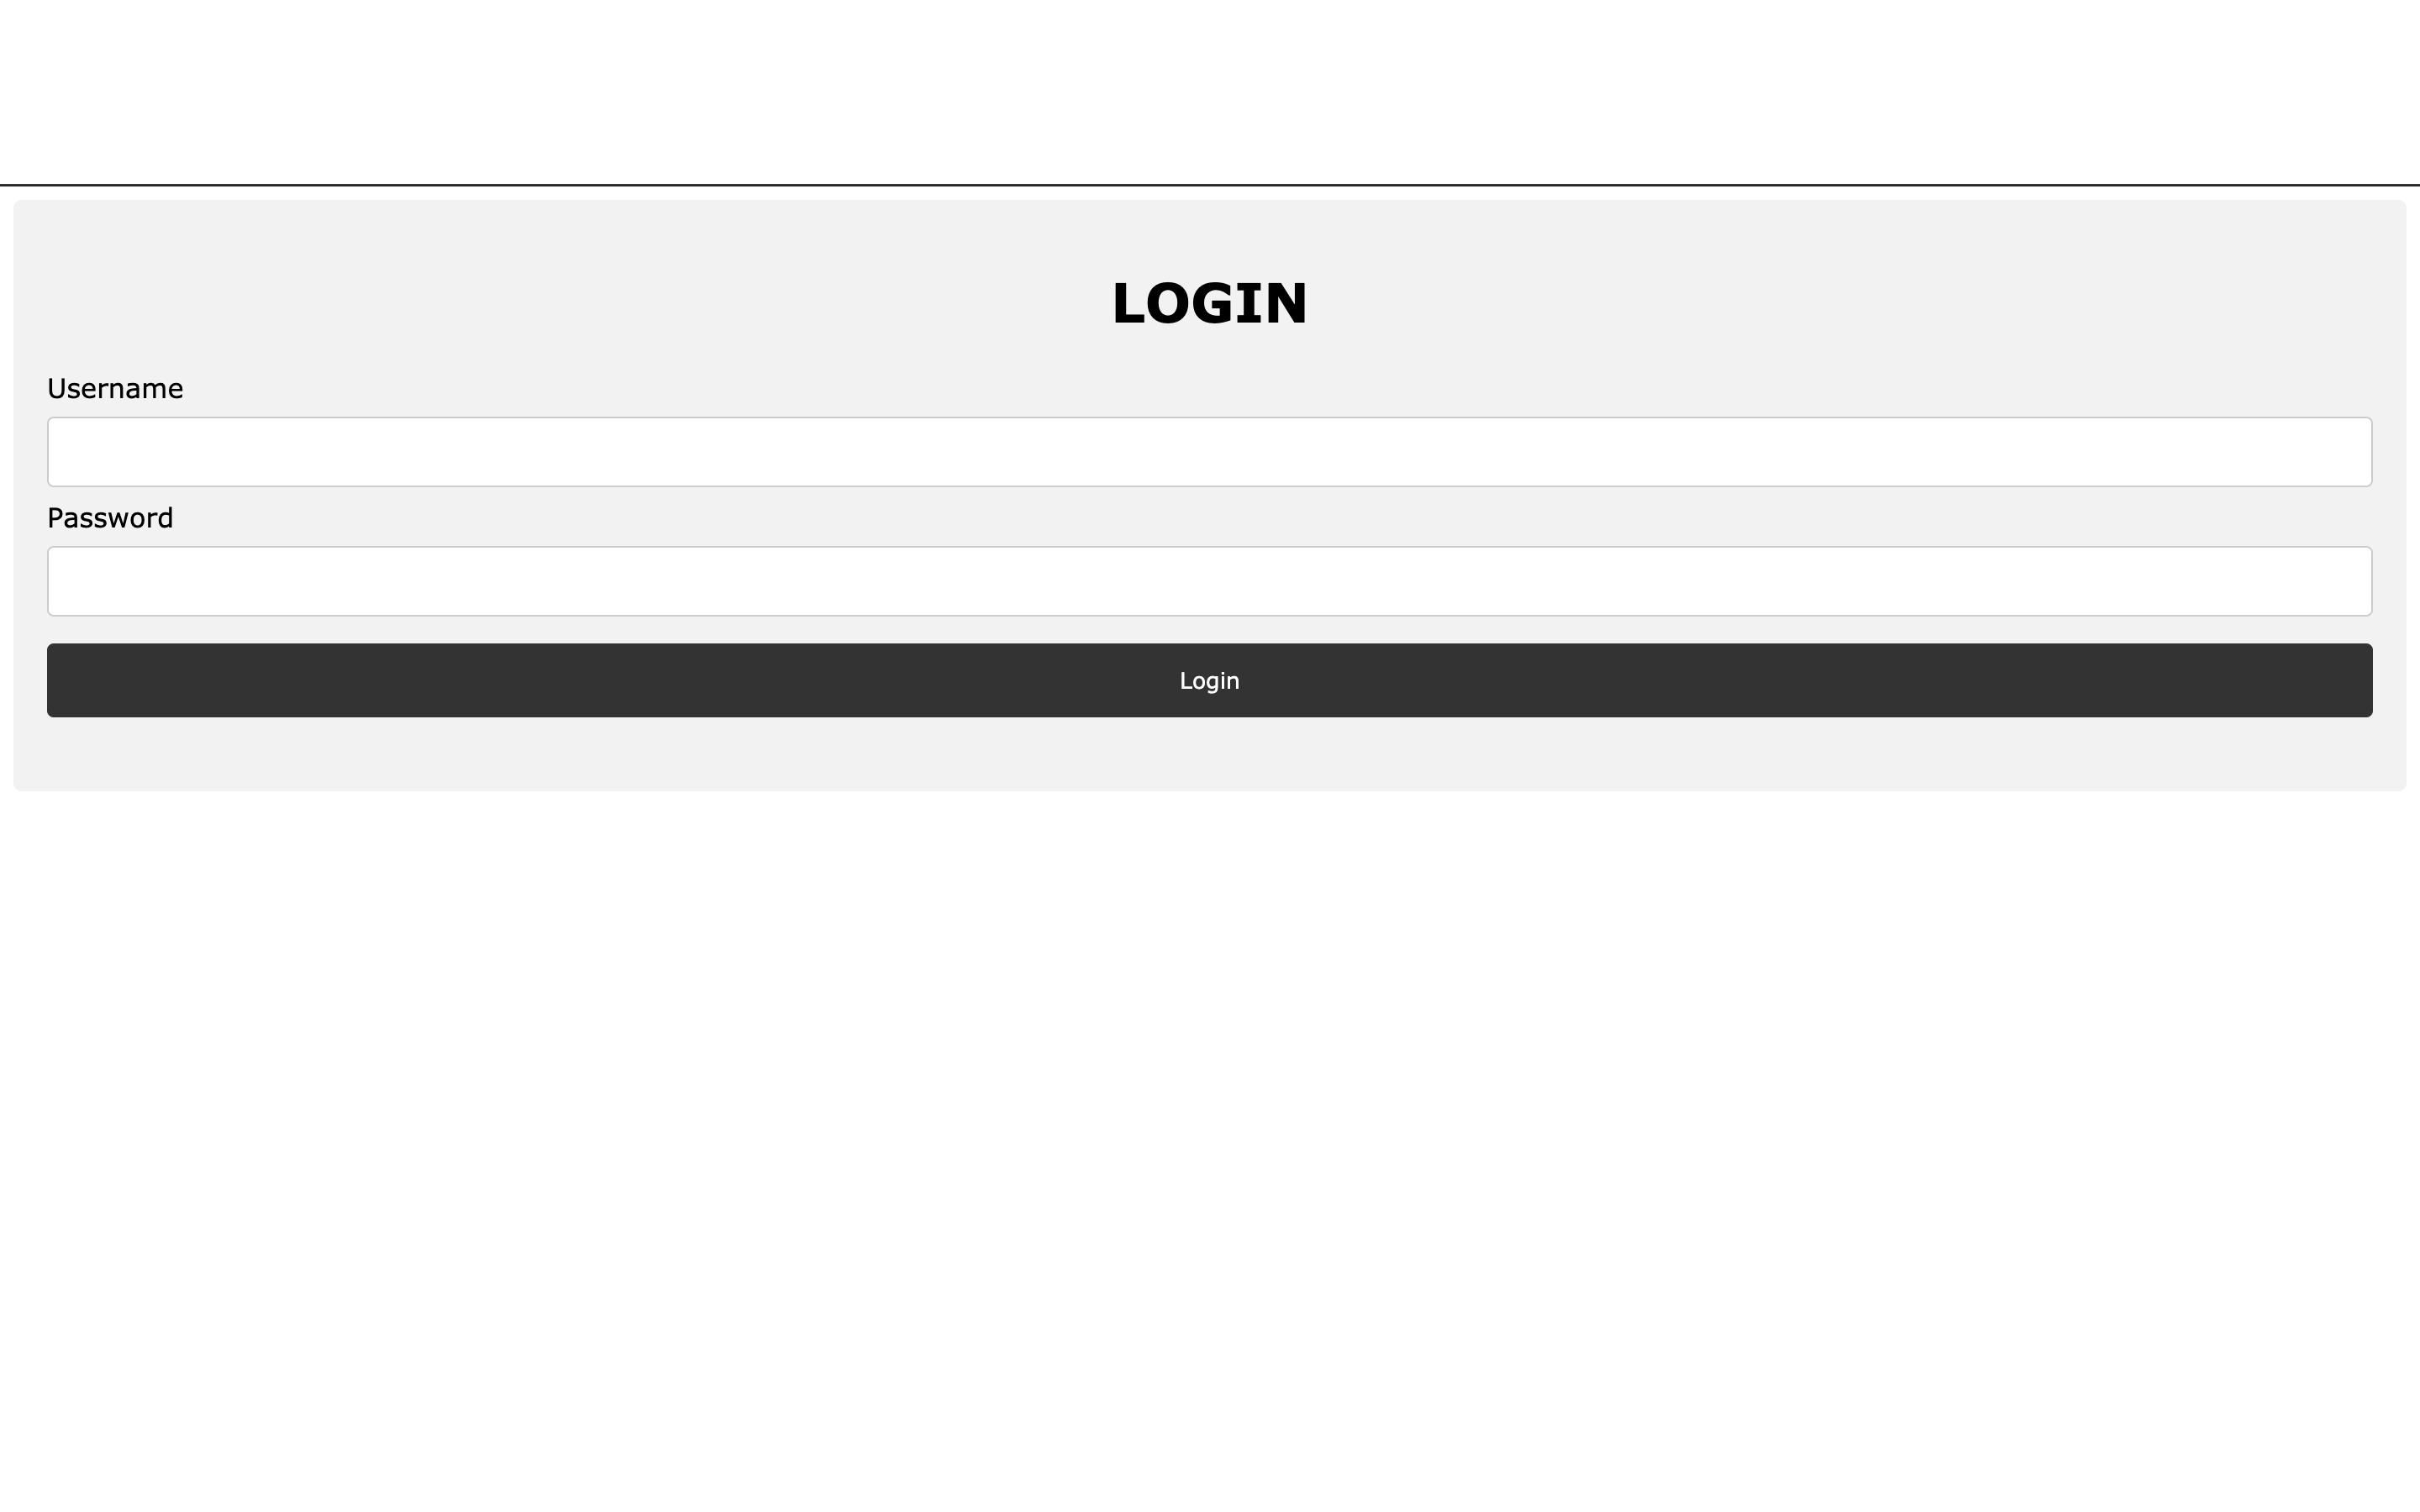
\includegraphics[scale=0.12]{res/images/login.png}
    \caption{Istantanea dello schermo di login}
\end{figure}
Nel caso in cui le credenziali inserite non risultassero corrette, verrà visualizzato un messaggio d'errore e sarà quindi necessario reinserire i dati di login.
\begin{figure}[H]
    \centering
    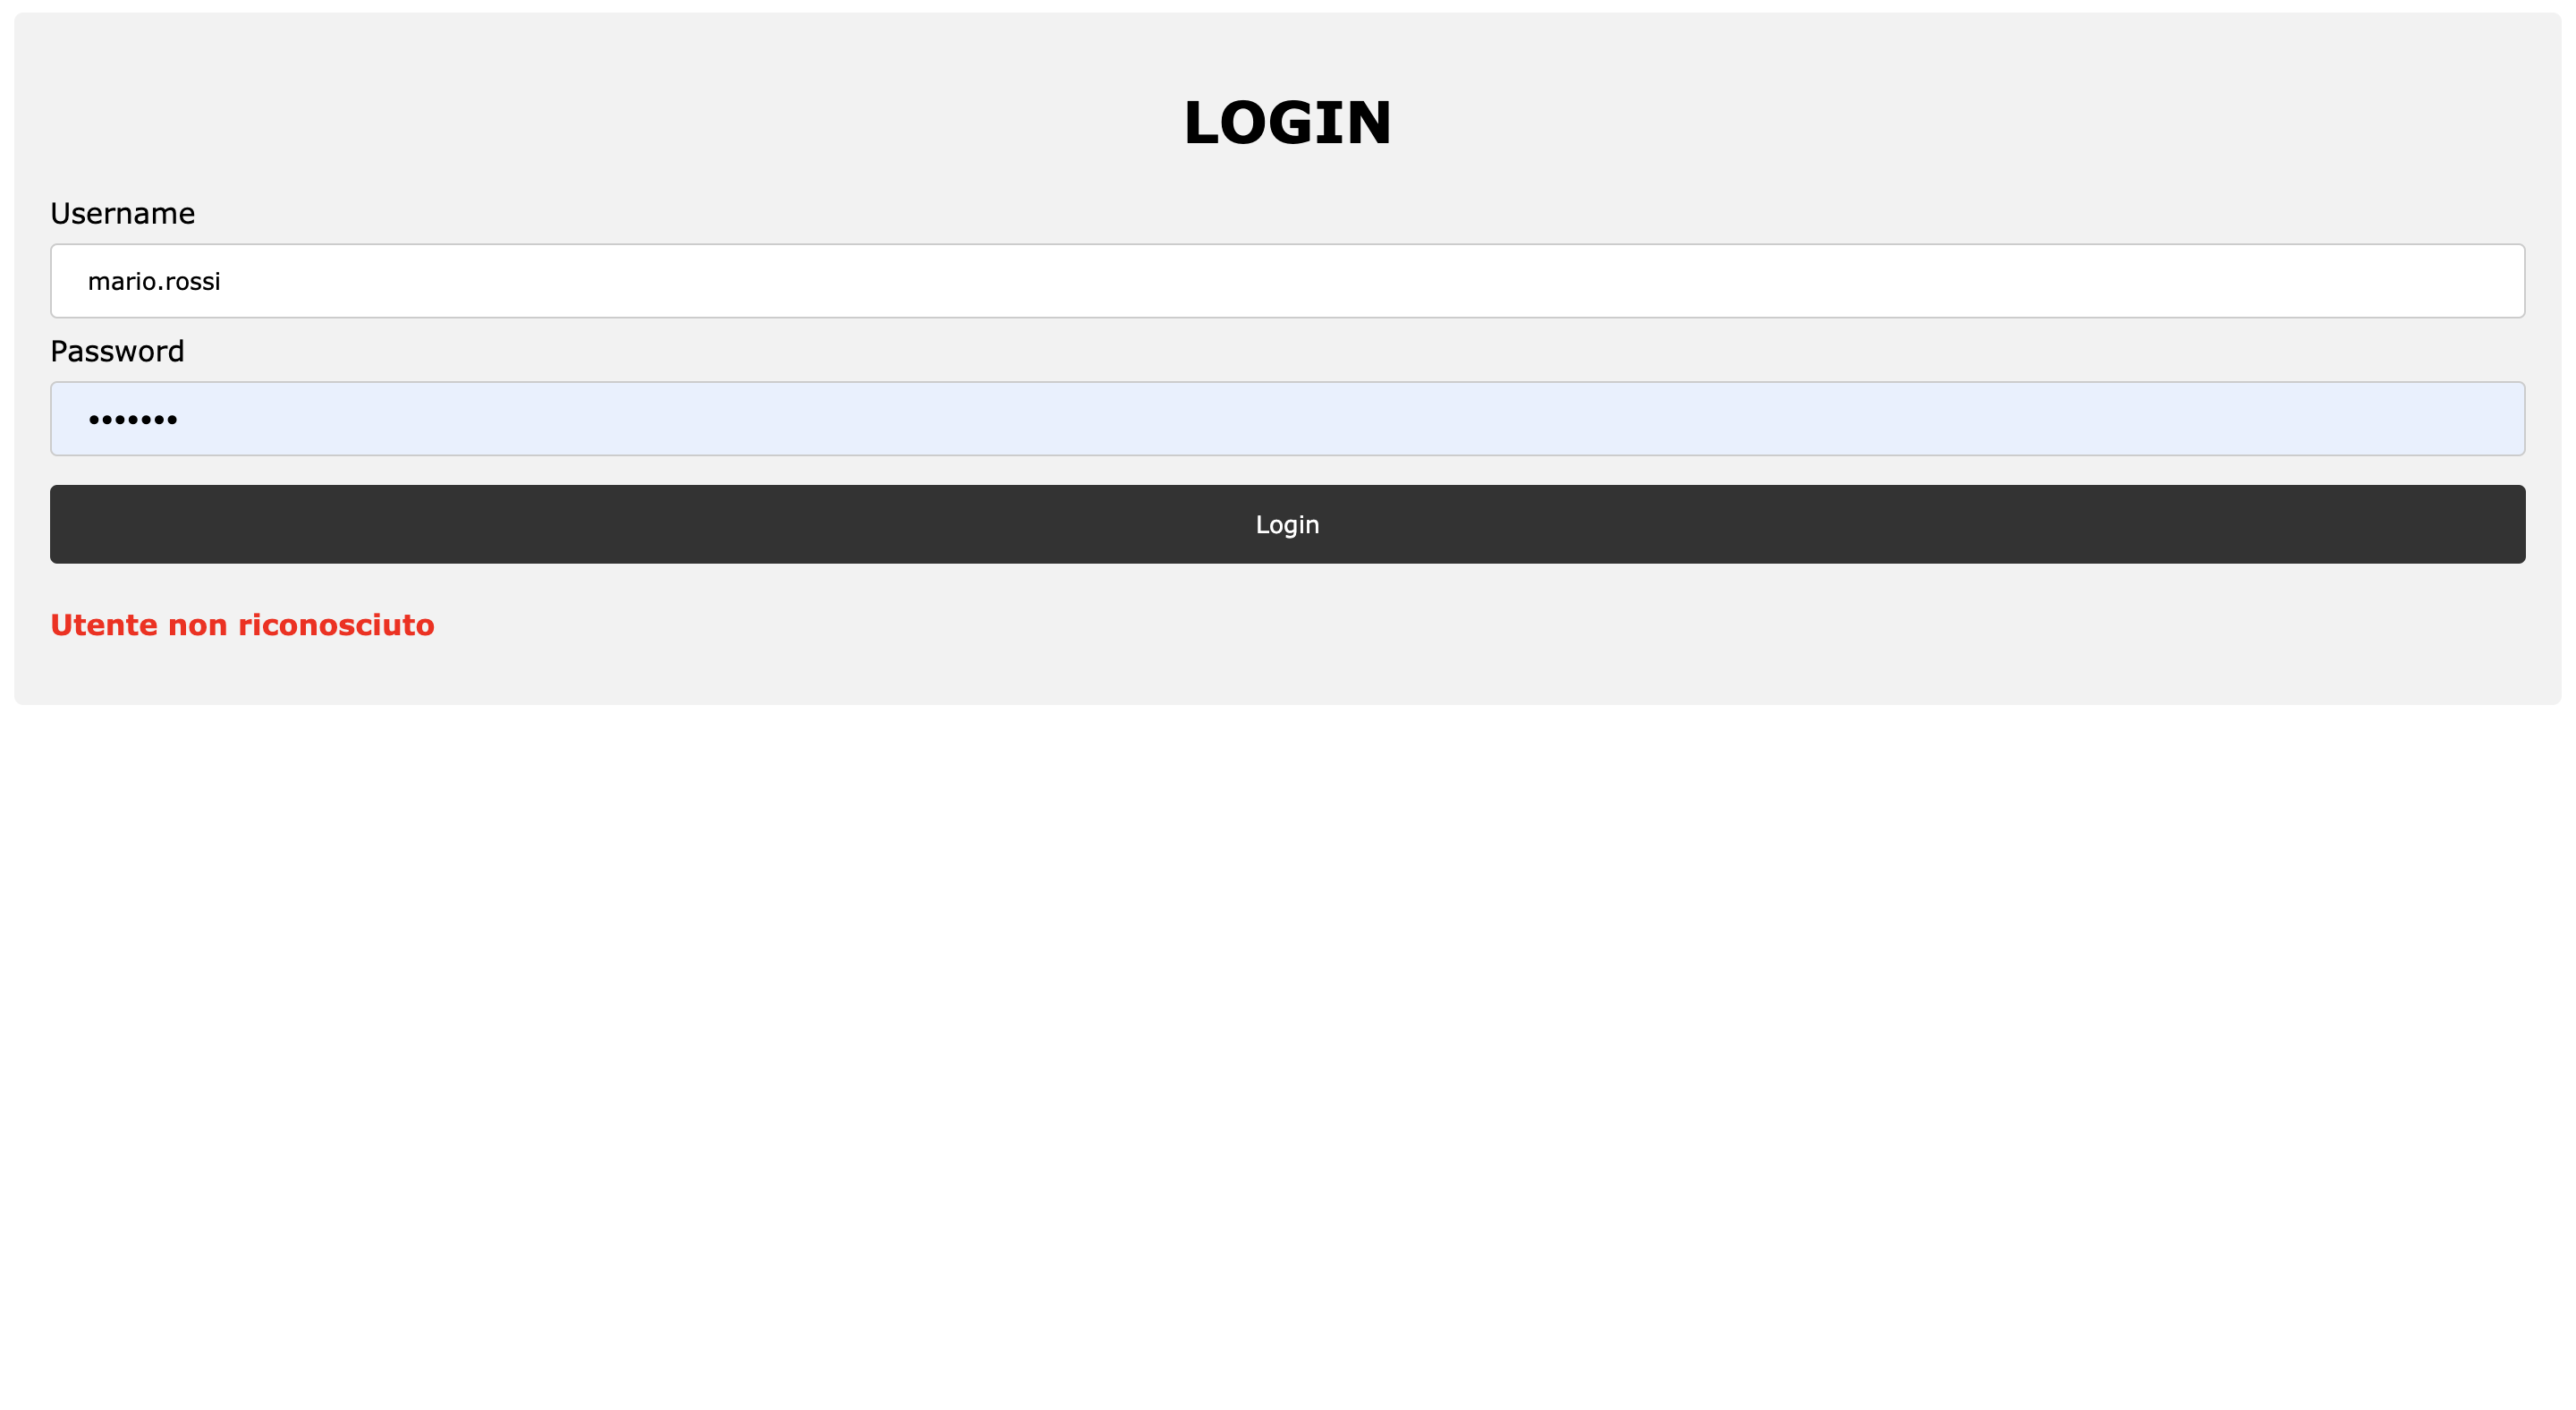
\includegraphics[scale=0.2]{res/images/login_errato.png}
    \caption{Istantanea dello schermo di login con errore}
\end{figure}

\subsection{Visualizzazione situazione in real time del magazzino}
\begin{itemize}
    \item Dopo l'autenticazione, tramite il menù selezionare il pulsante "Mappa";
    \begin{figure}[H]
        \centering
        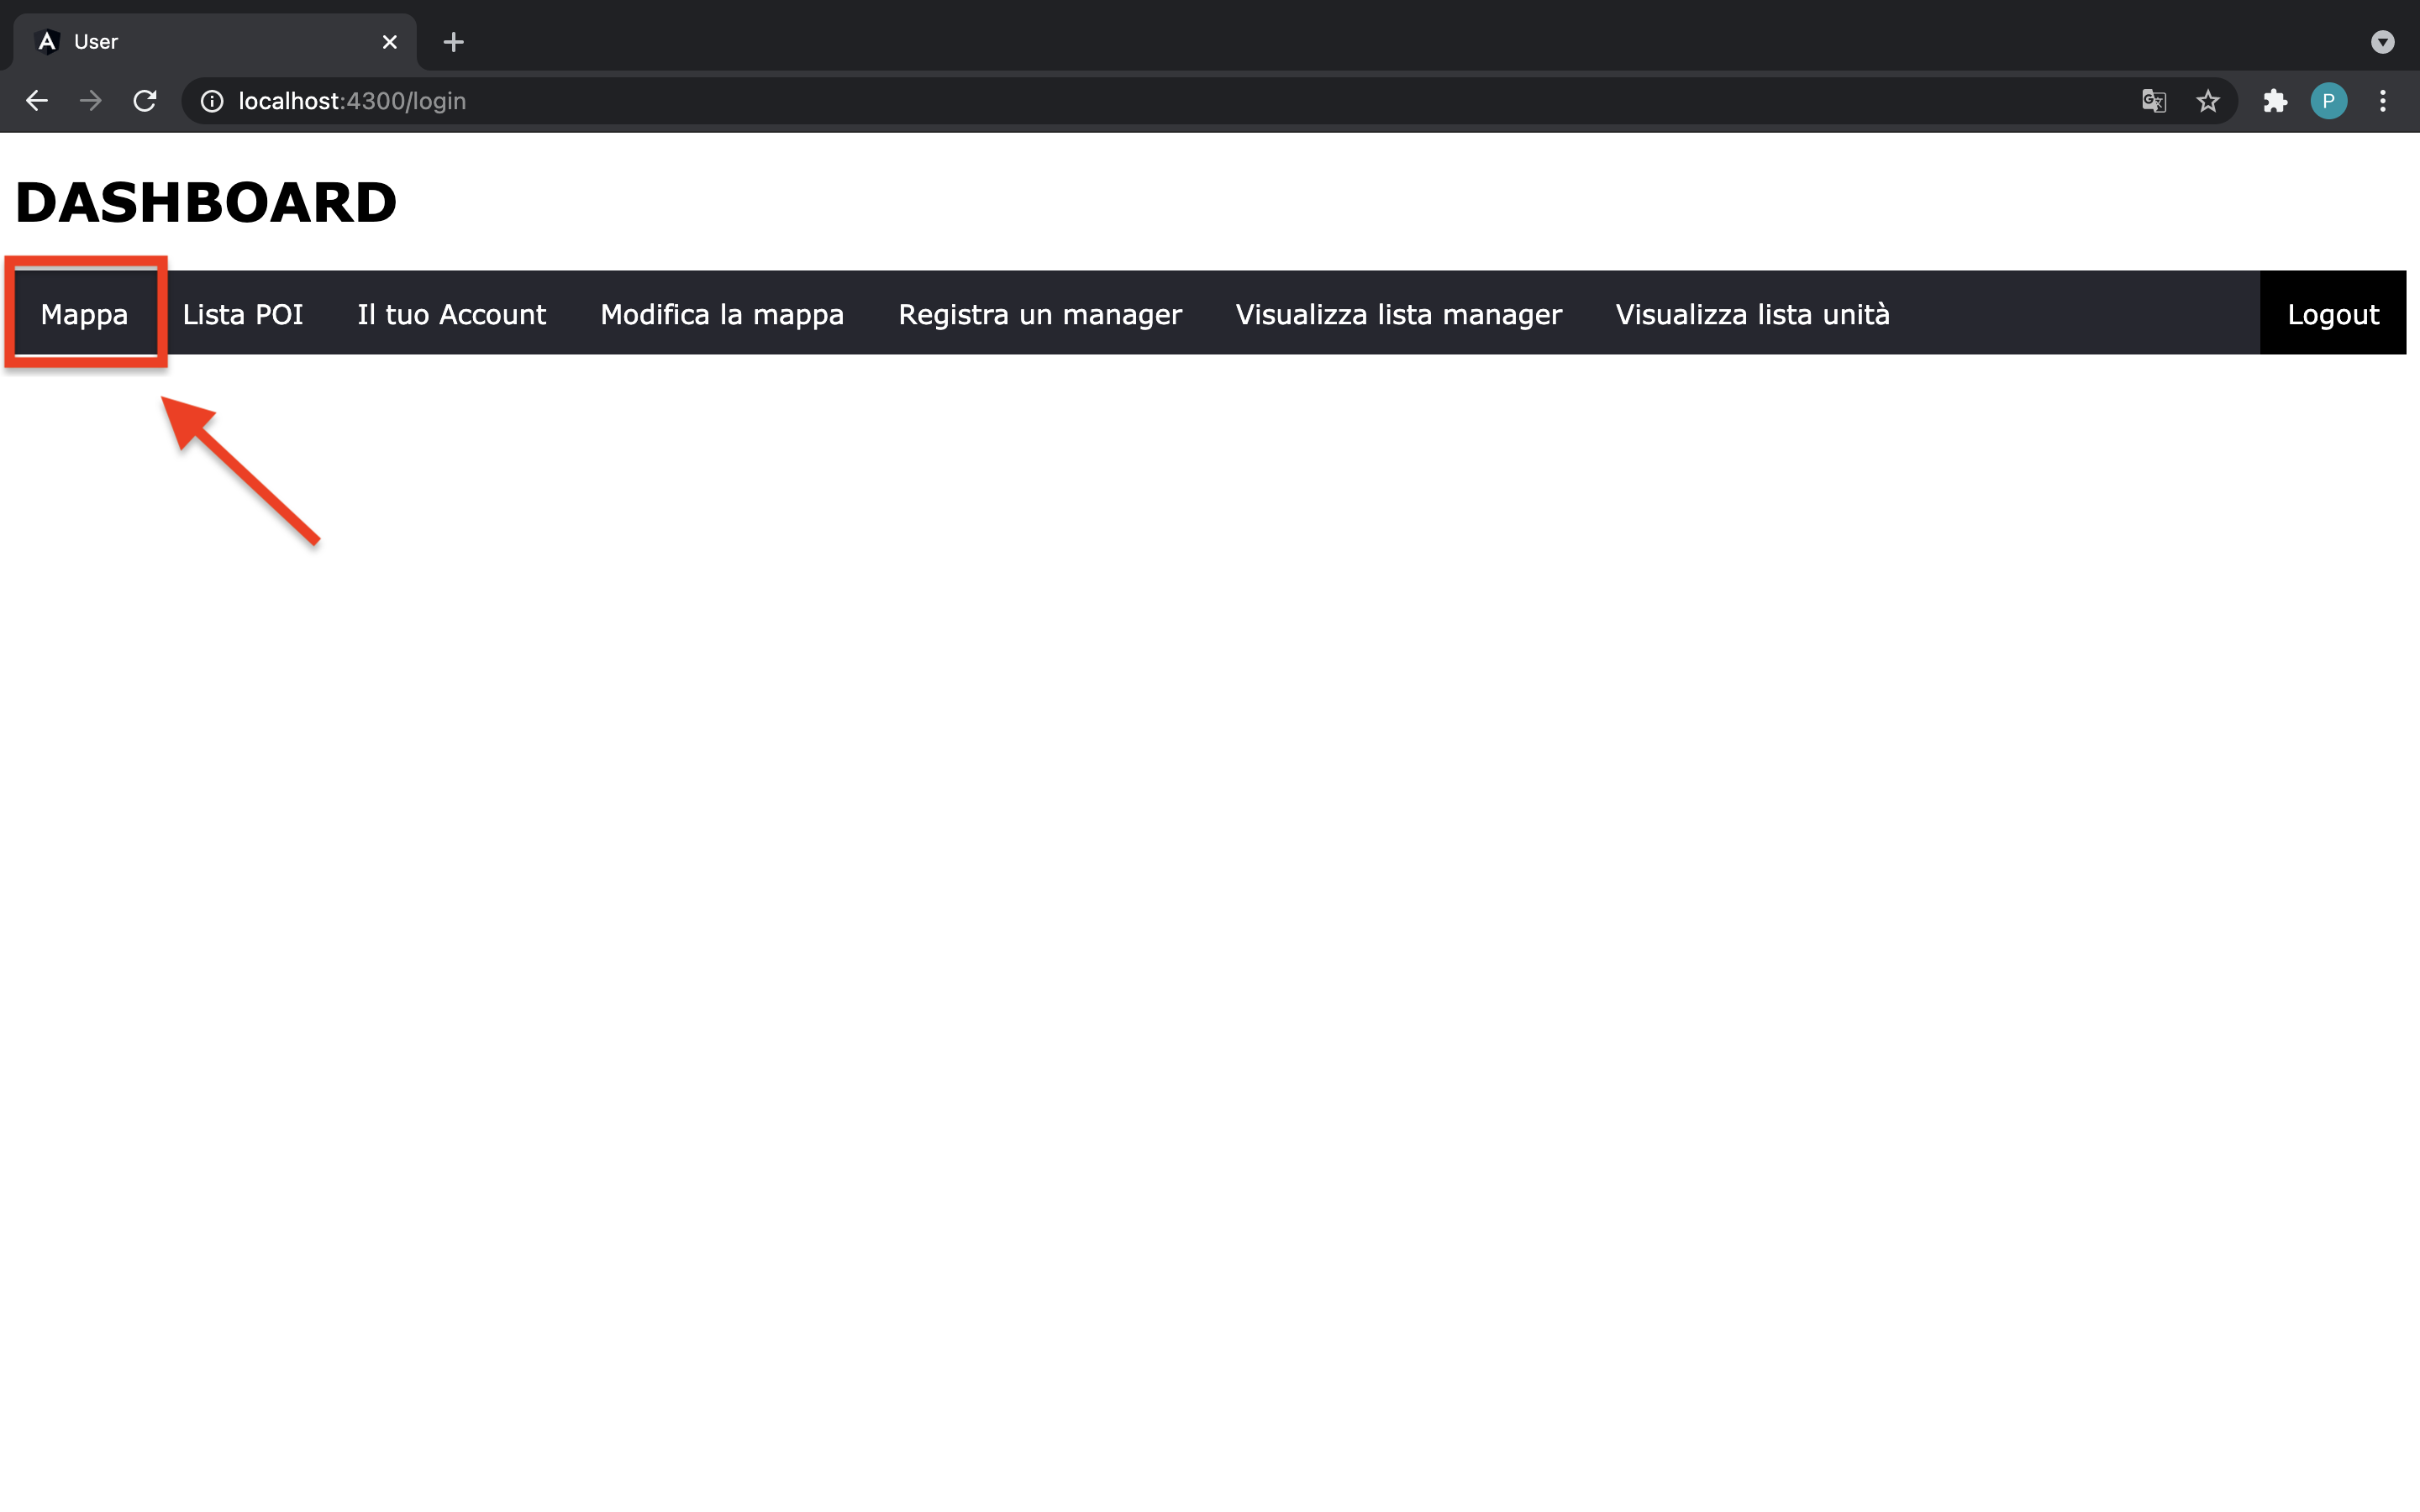
\includegraphics[scale=0.12]{res/images/dashboard1.png}
        \caption{Istantanea dello schermo con indicazione per la visualizzazione della mappa in real time}
    \end{figure}
    \item viene visualizzata la planimetria del magazzino e la rappresentazione dei muletti che si spostano tramite l'icona blu e il proprio id;
    \item la tabella a destra rappresenta le varie unità con le relative liste di task che stanno soddisfacendo.
    
\end{itemize}

\begin{figure}[H]
    \centering
    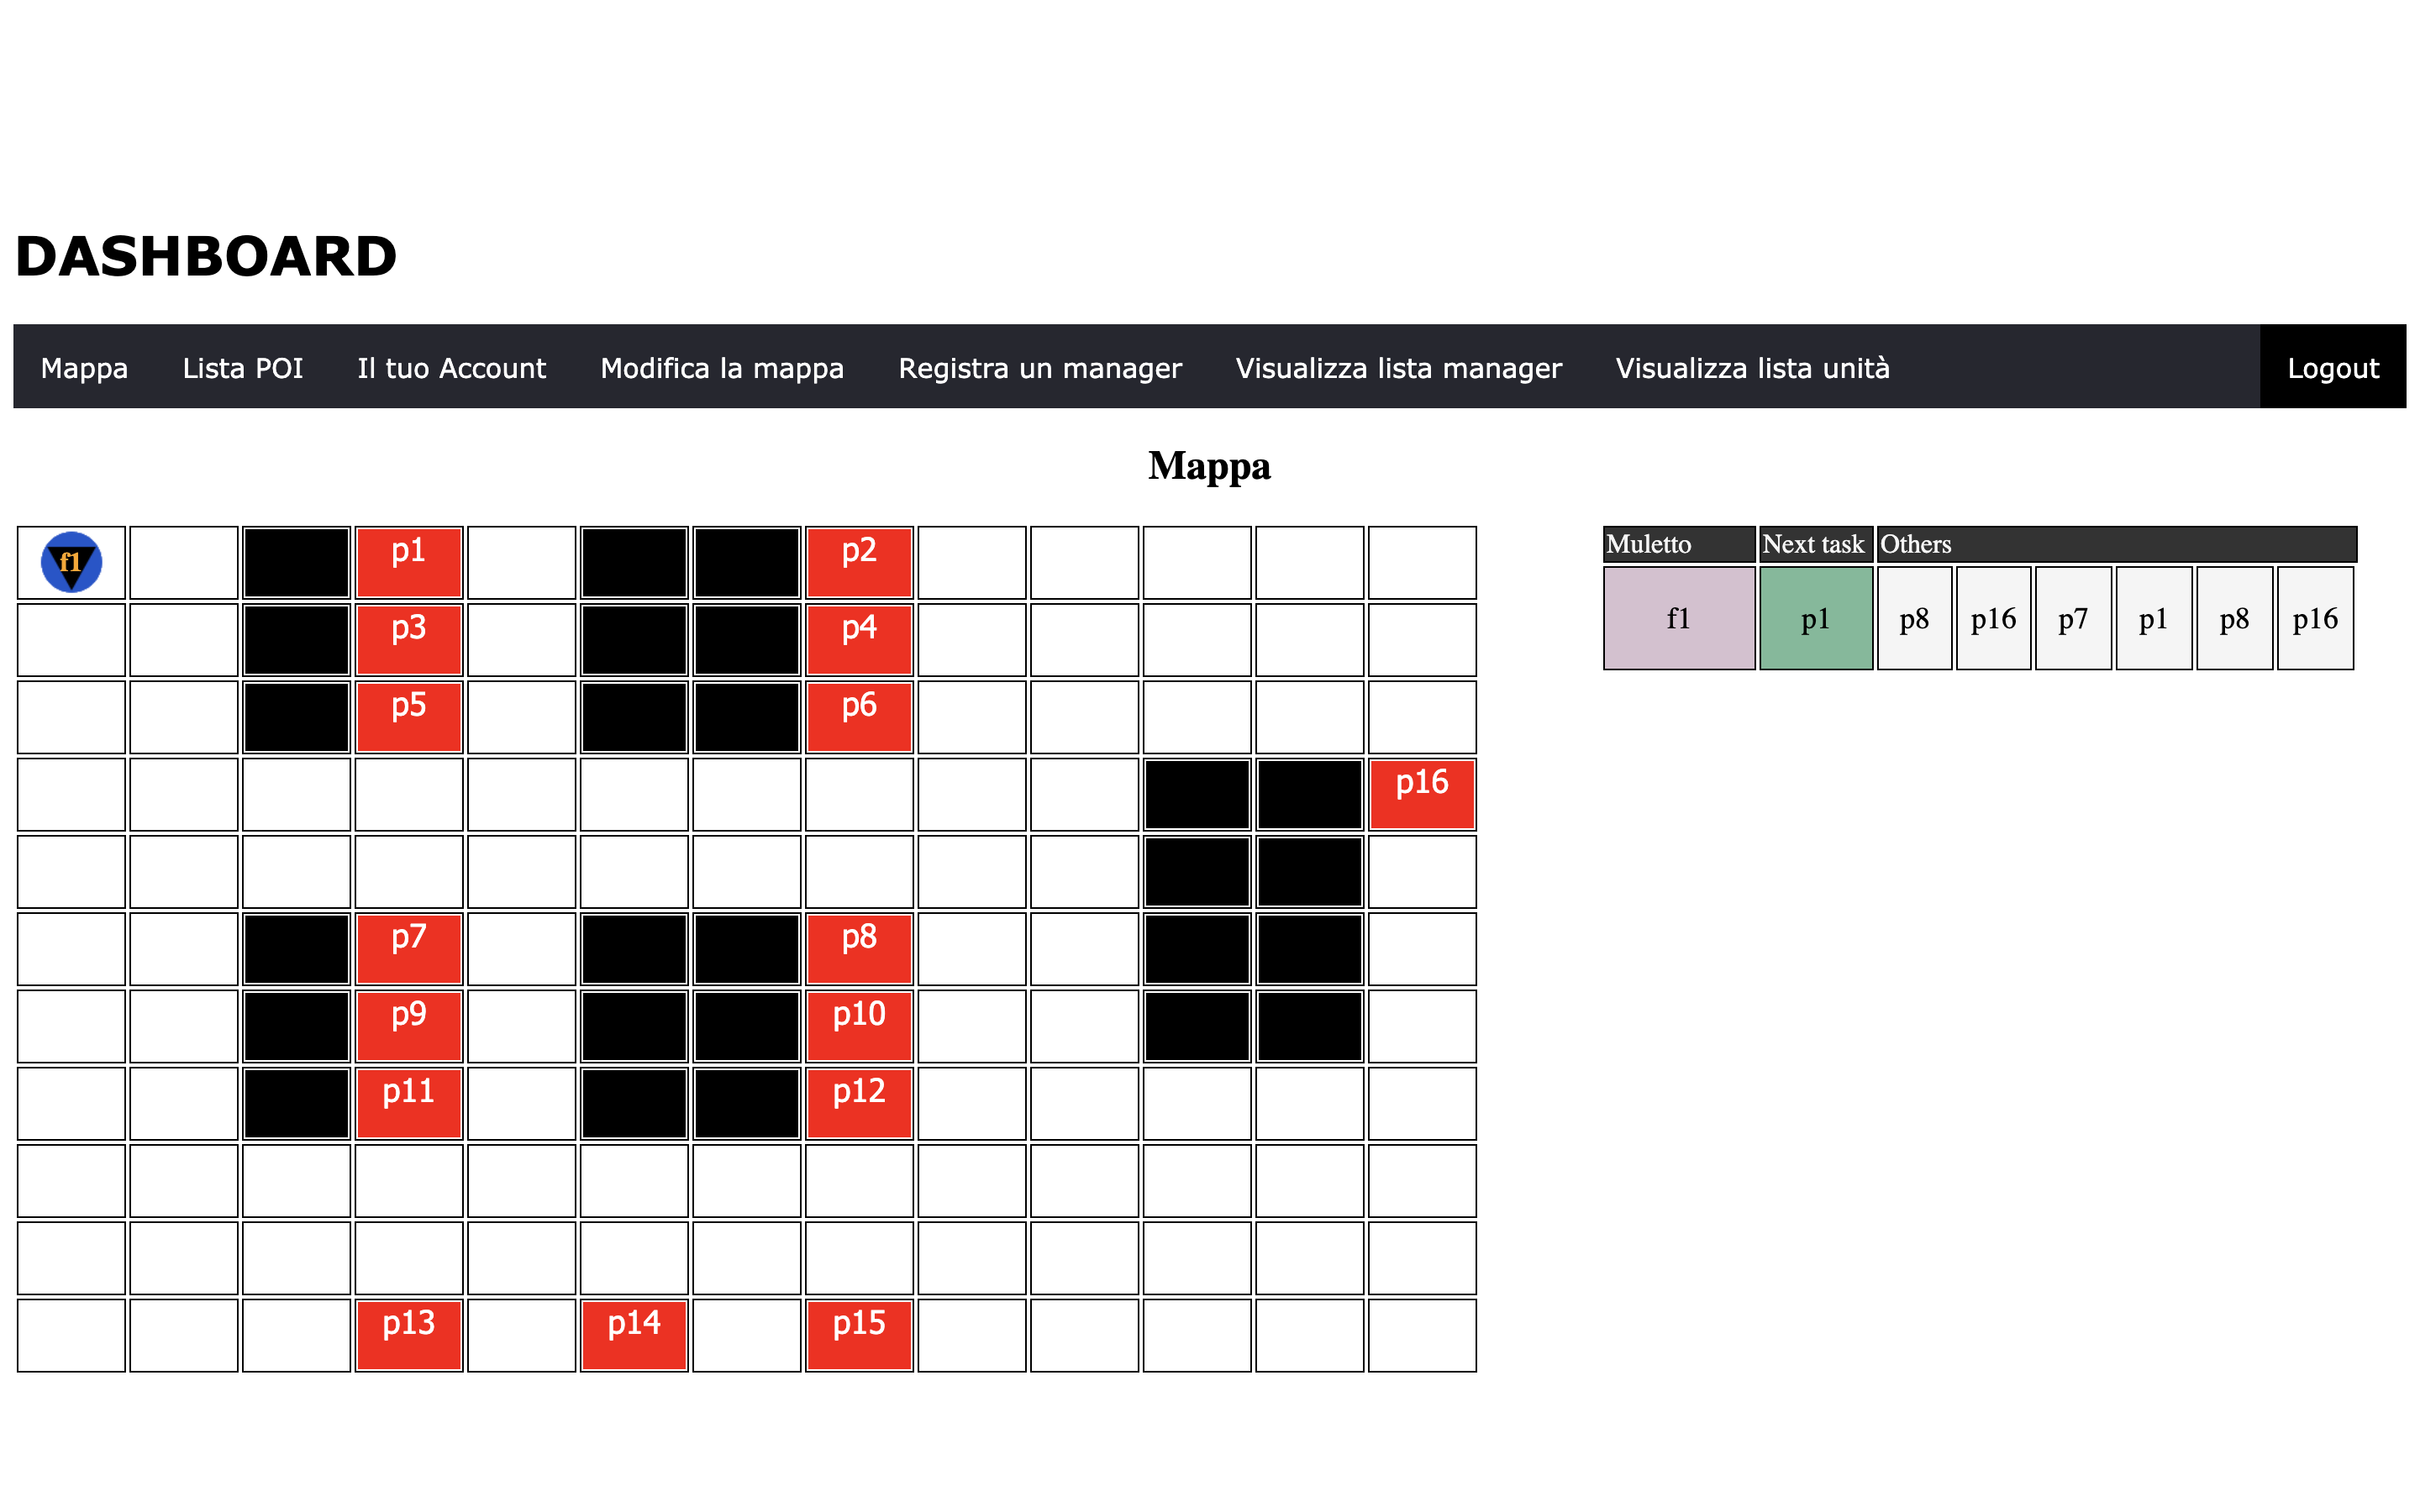
\includegraphics[scale=0.12]{res/images/map_user.png}
    \caption{Istantanea dello schermo visualizzazione in real time del magazzino}
\end{figure}

\subsection{Visualizzazione lista completa punti di interesse}
\begin{itemize}
    \item Dopo l'autenticazione, tramite il menù selezionare il pulsante "Lista POI";
    \begin{figure}[H]
        \centering
        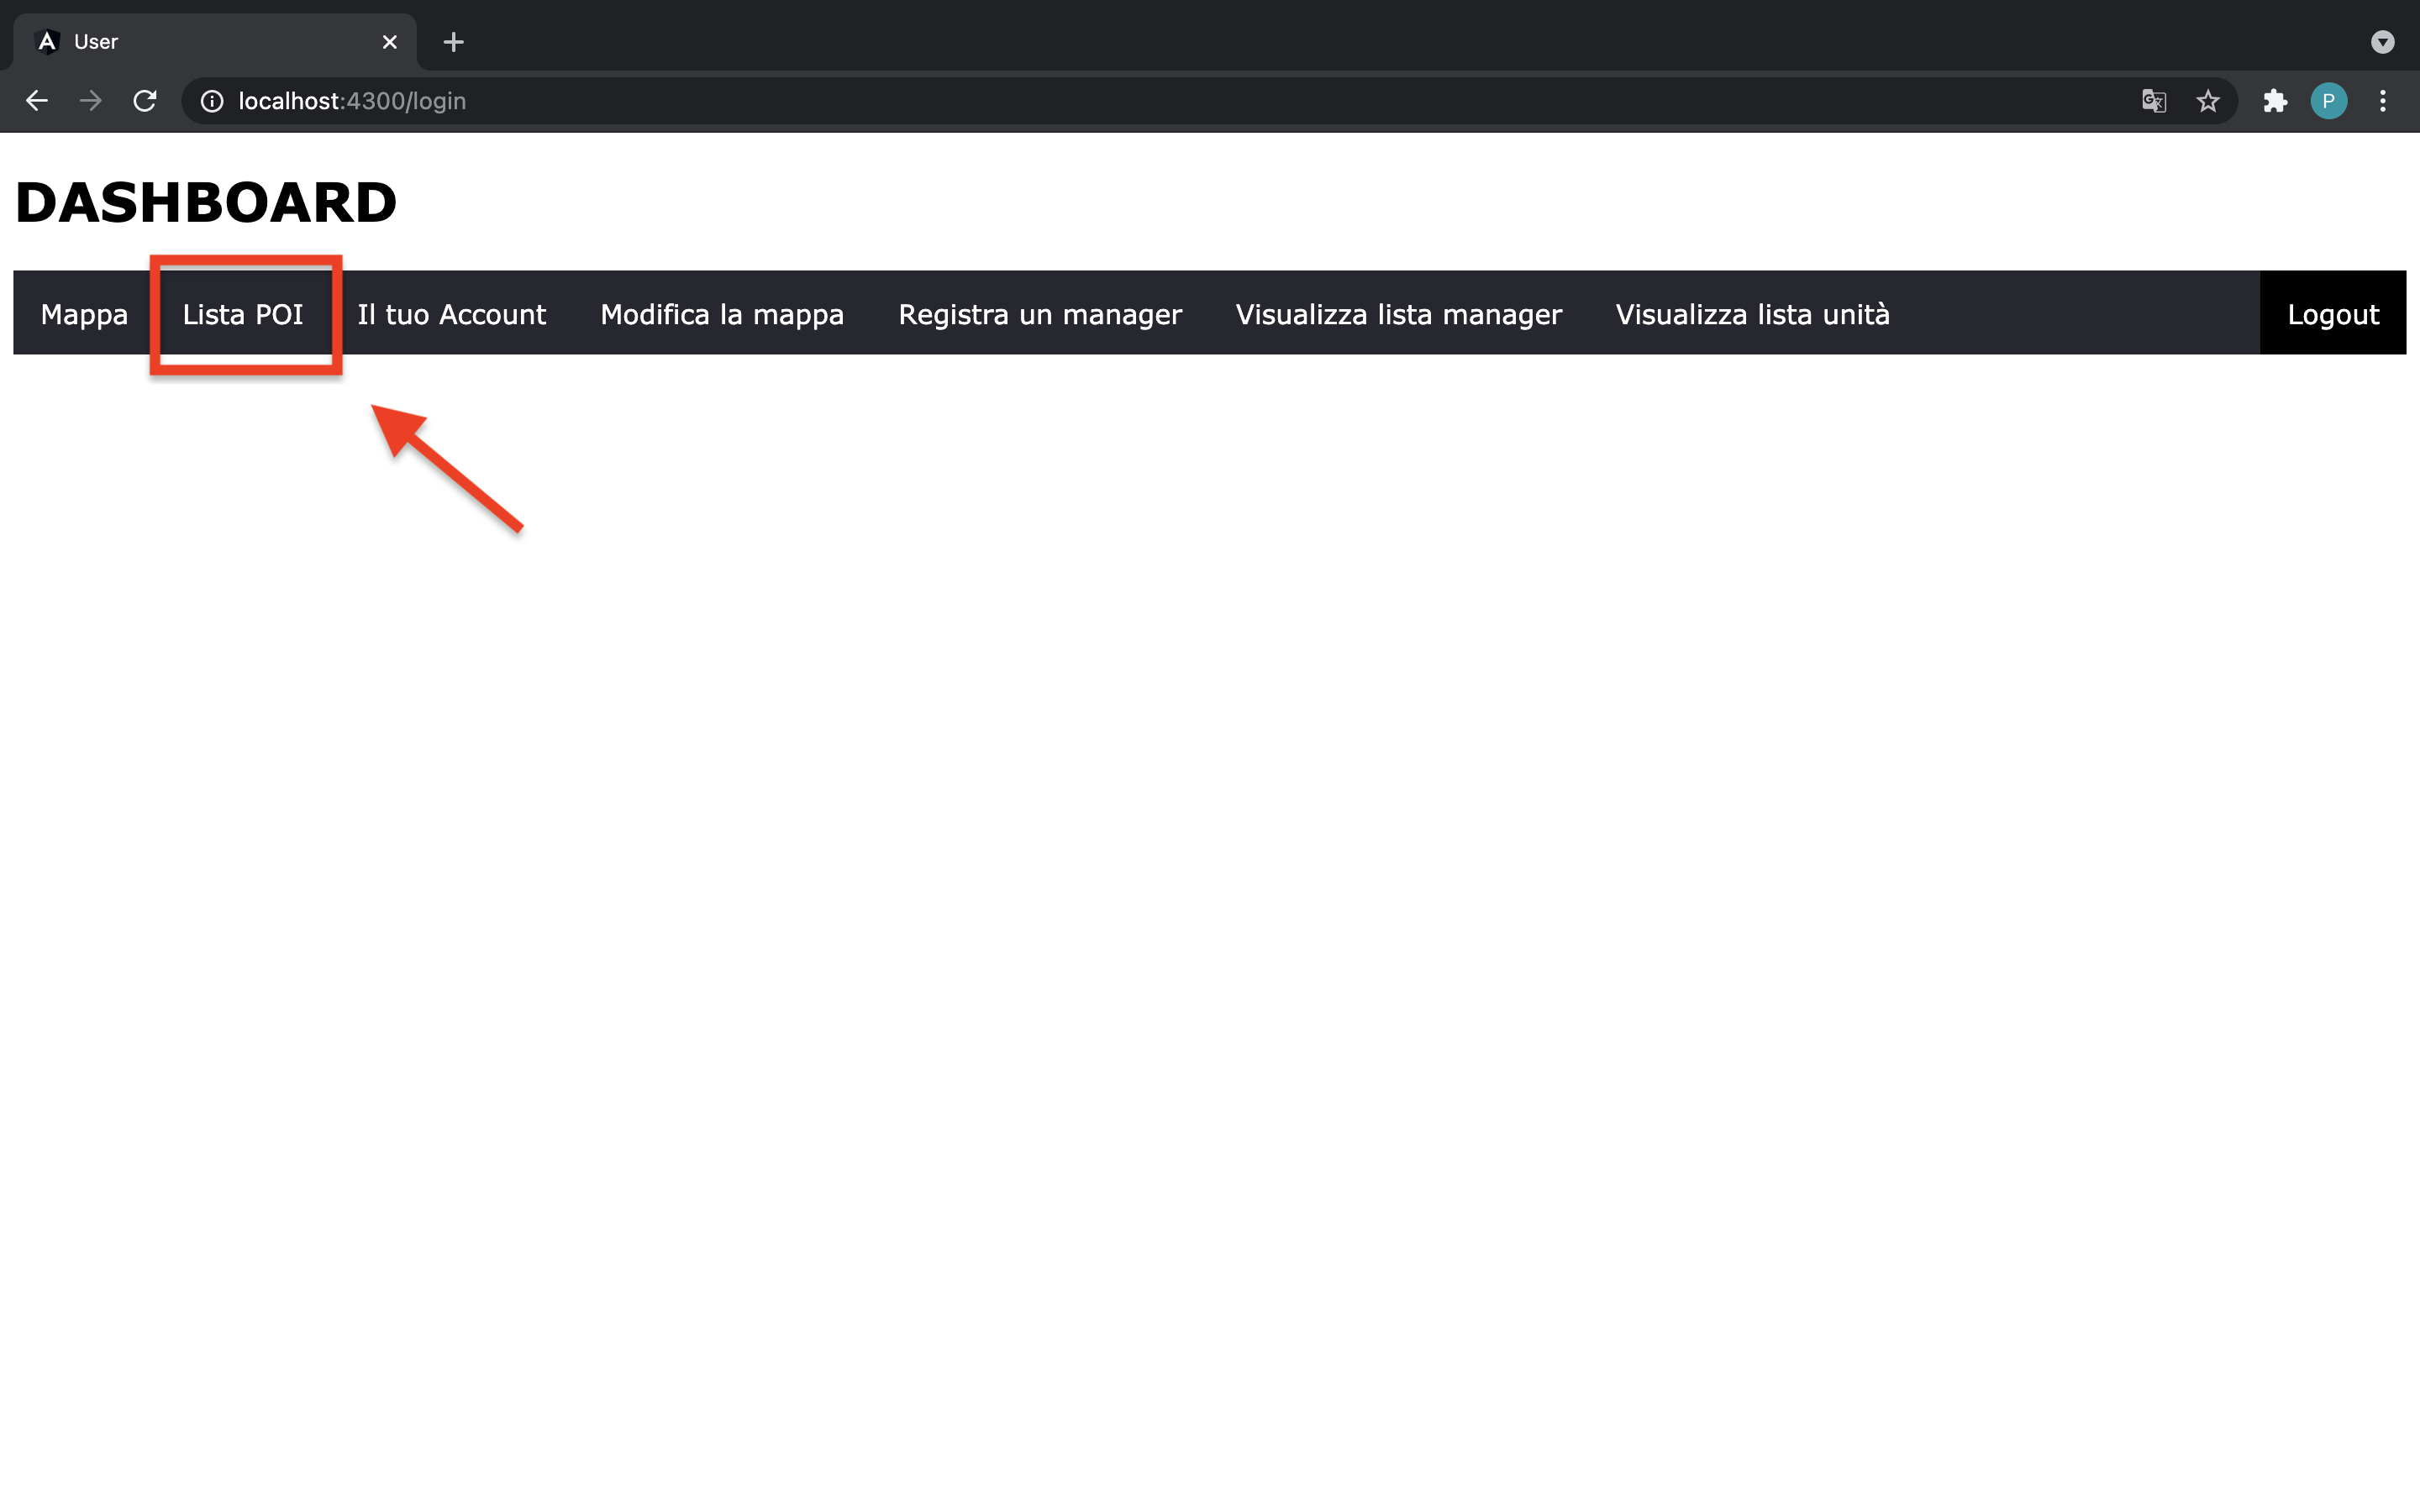
\includegraphics[scale=0.12]{res/images/dashboard2.png}
        \caption{Istantanea dello schermo dashboard con indicazione per la visualizzazione di tutti i POI}
    \end{figure}
    \item si viene indirizzati alla pagina con l'elenco di tutti i punti di interesse presenti nel magazzino con il relativo id, nome e tipo.

\end{itemize}

\begin{figure}[H]
    \centering
    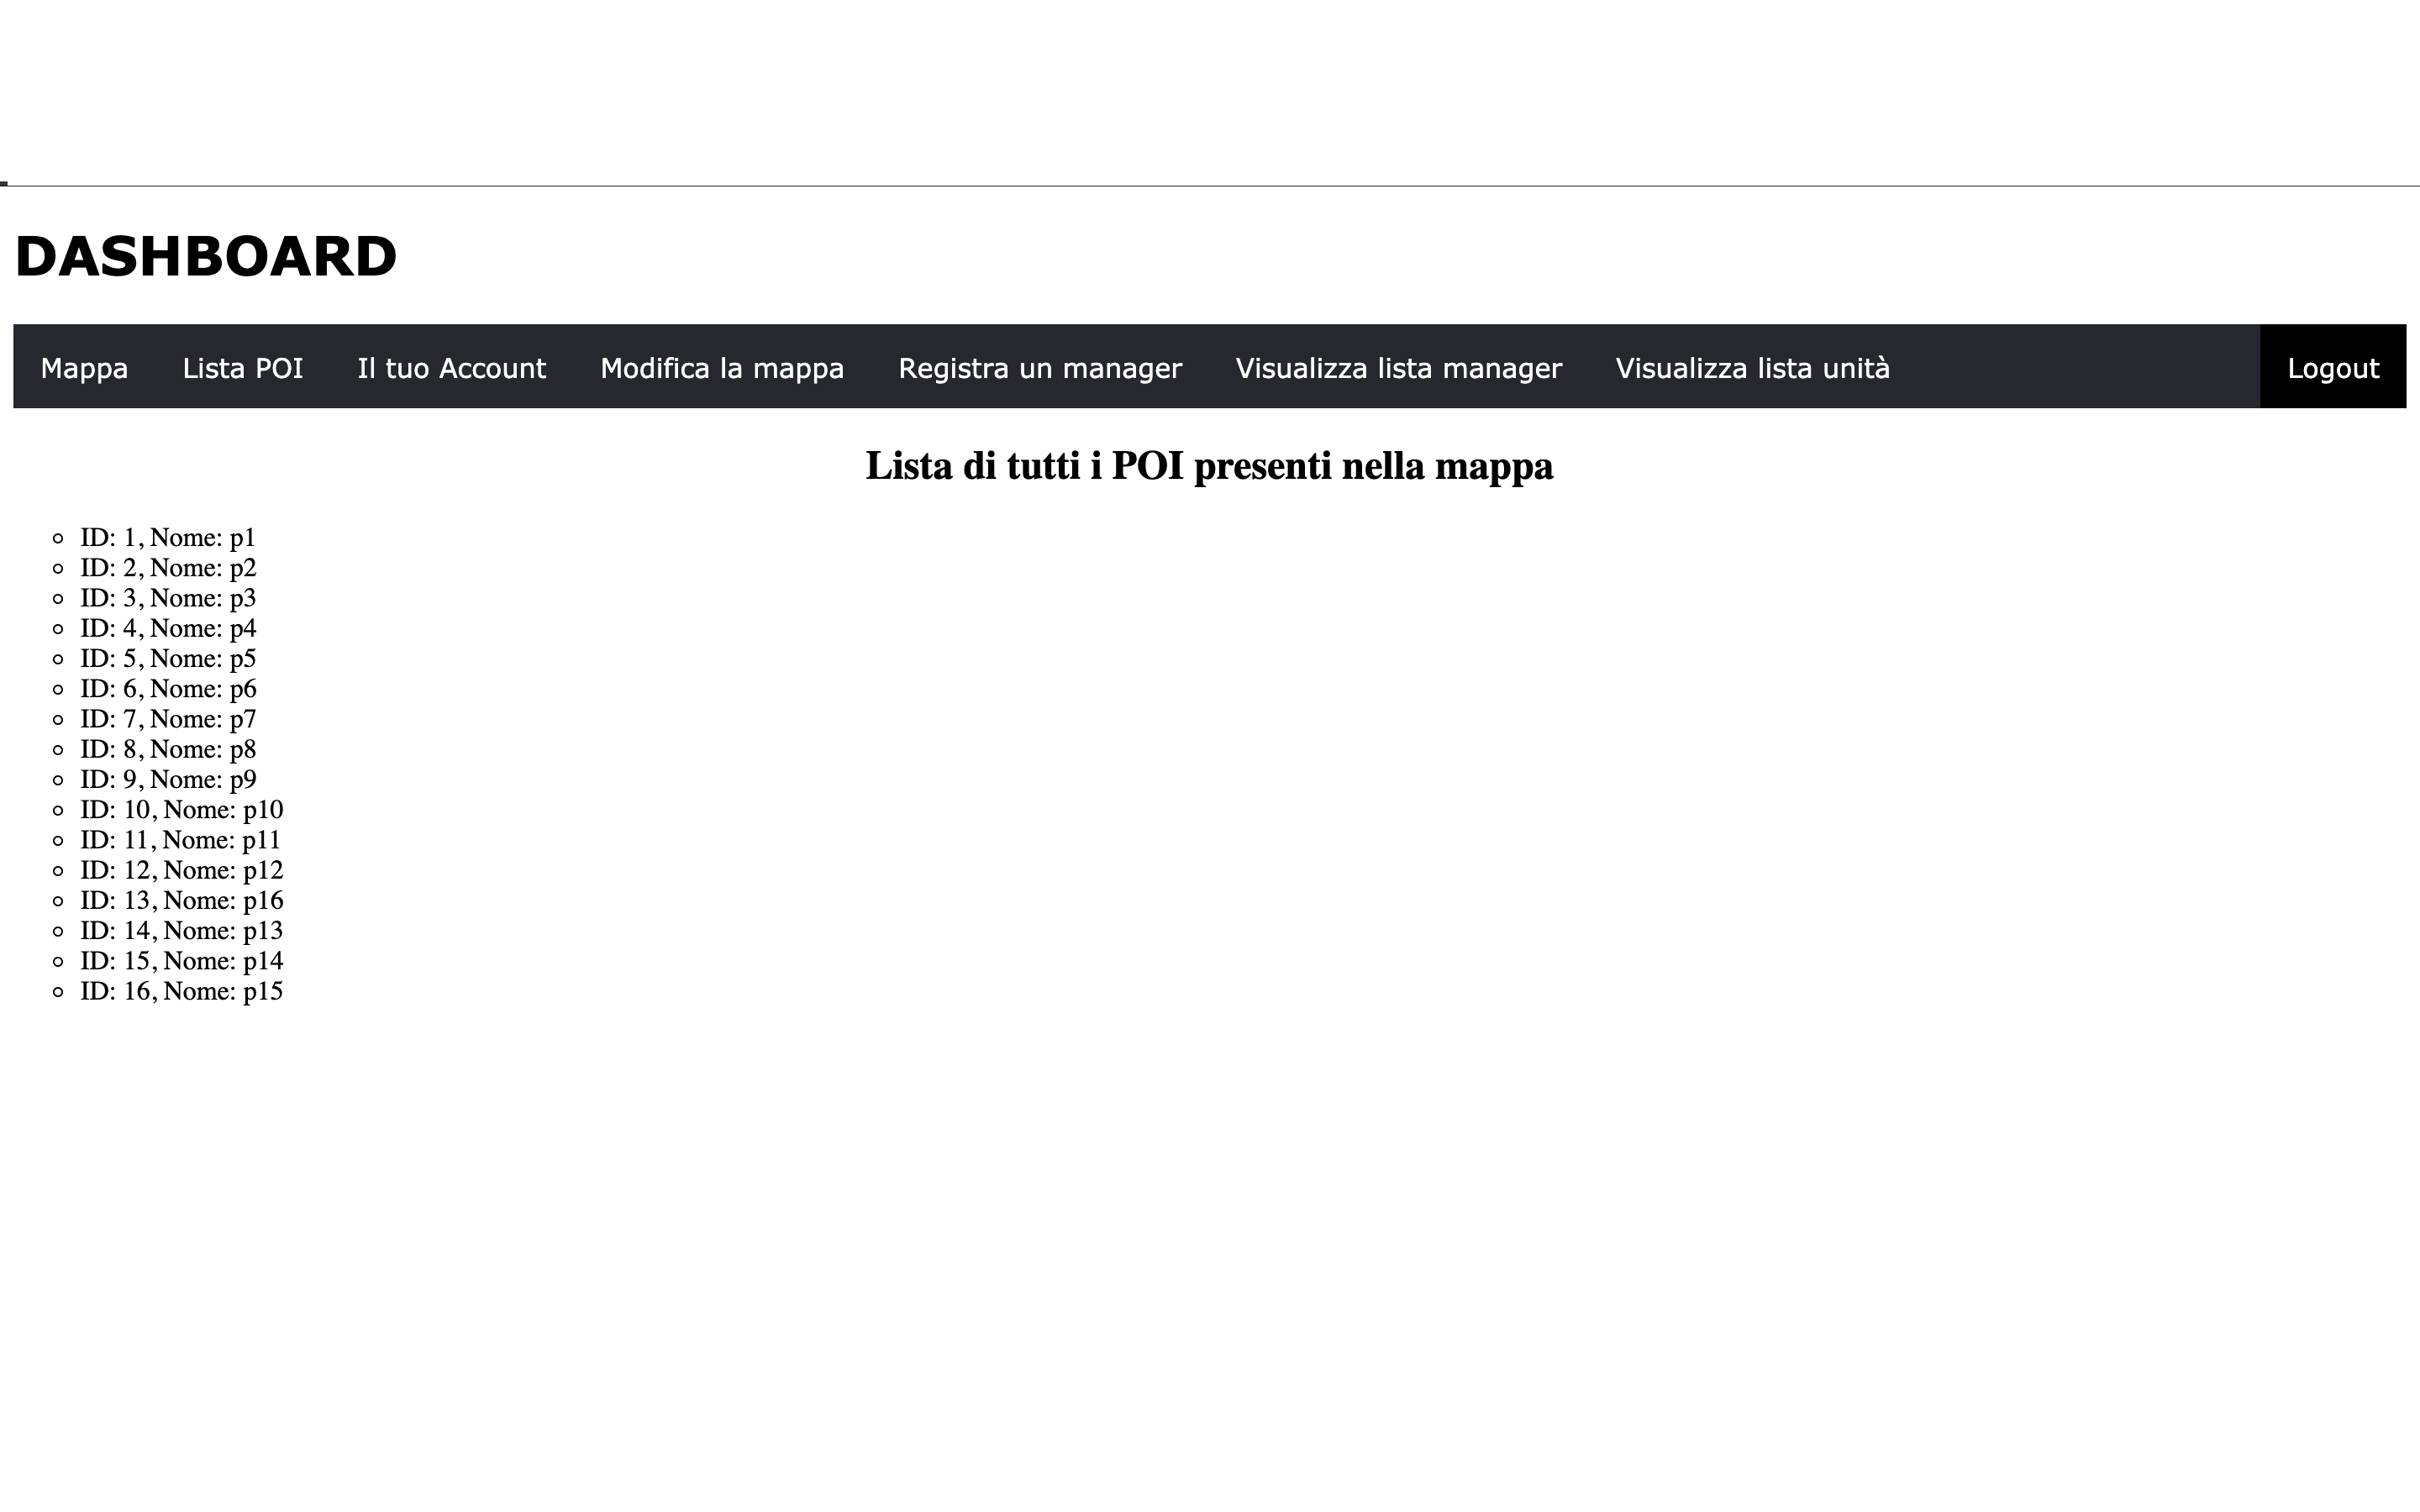
\includegraphics[scale=0.12]{res/images/listpoi_user.png}
    \caption{Istantanea dello schermo visualizzazione lista punti di interesse}
\end{figure}

\subsection{Visualizzazione dati del proprio profilo e modifica}
\begin{itemize}
    \item Dopo l'autenticazione, tramite il menù selezionare il pulsante "Il tuo Account";
    \begin{figure}[H]
        \centering
        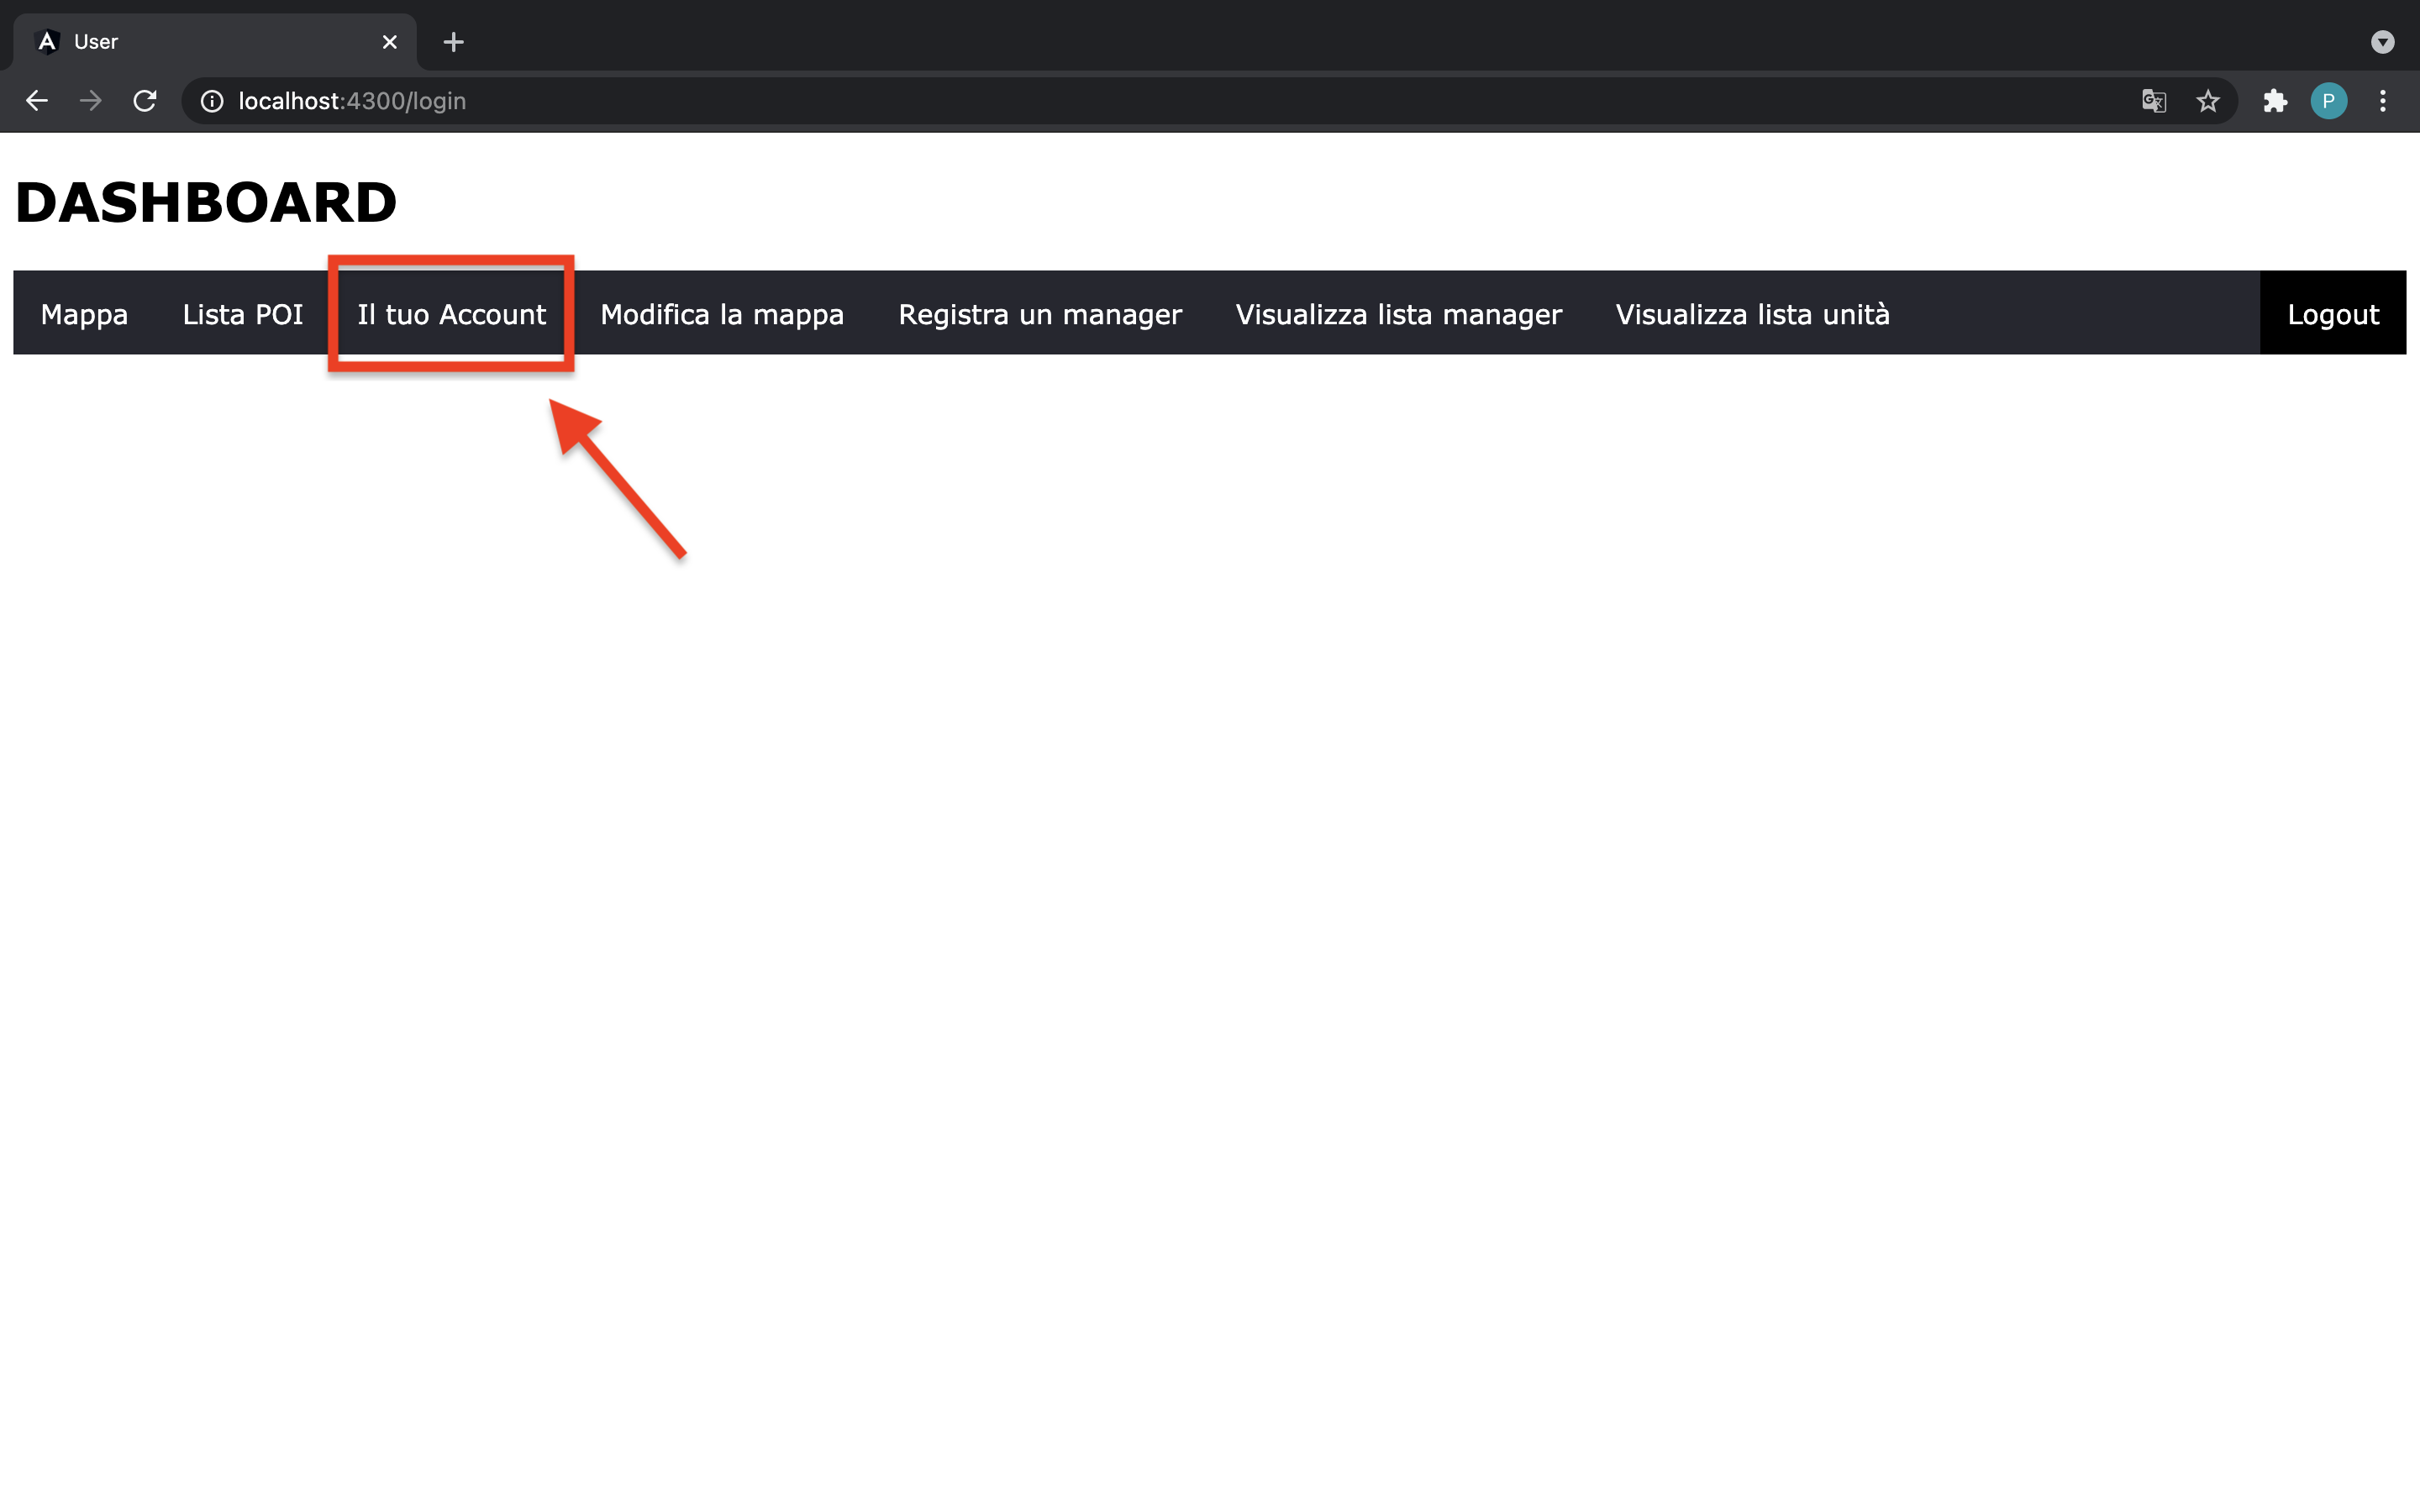
\includegraphics[scale=0.12]{res/images/dashboard3.png}
        \caption{Istantanea dello schermo dashboard con indicazione per la visualizzazione del proprio profilo}
    \end{figure}
    
    \item si viene indirizzati alla pagina con i propri dati utente: Nome, Cognome e Password;
    \item se si desidera modificare alcuni campi, è necessario scrivere nell'apposito form i nuovi dati e premere il pulsante "Salva modifiche".
    \begin{figure}[H]
        \centering
        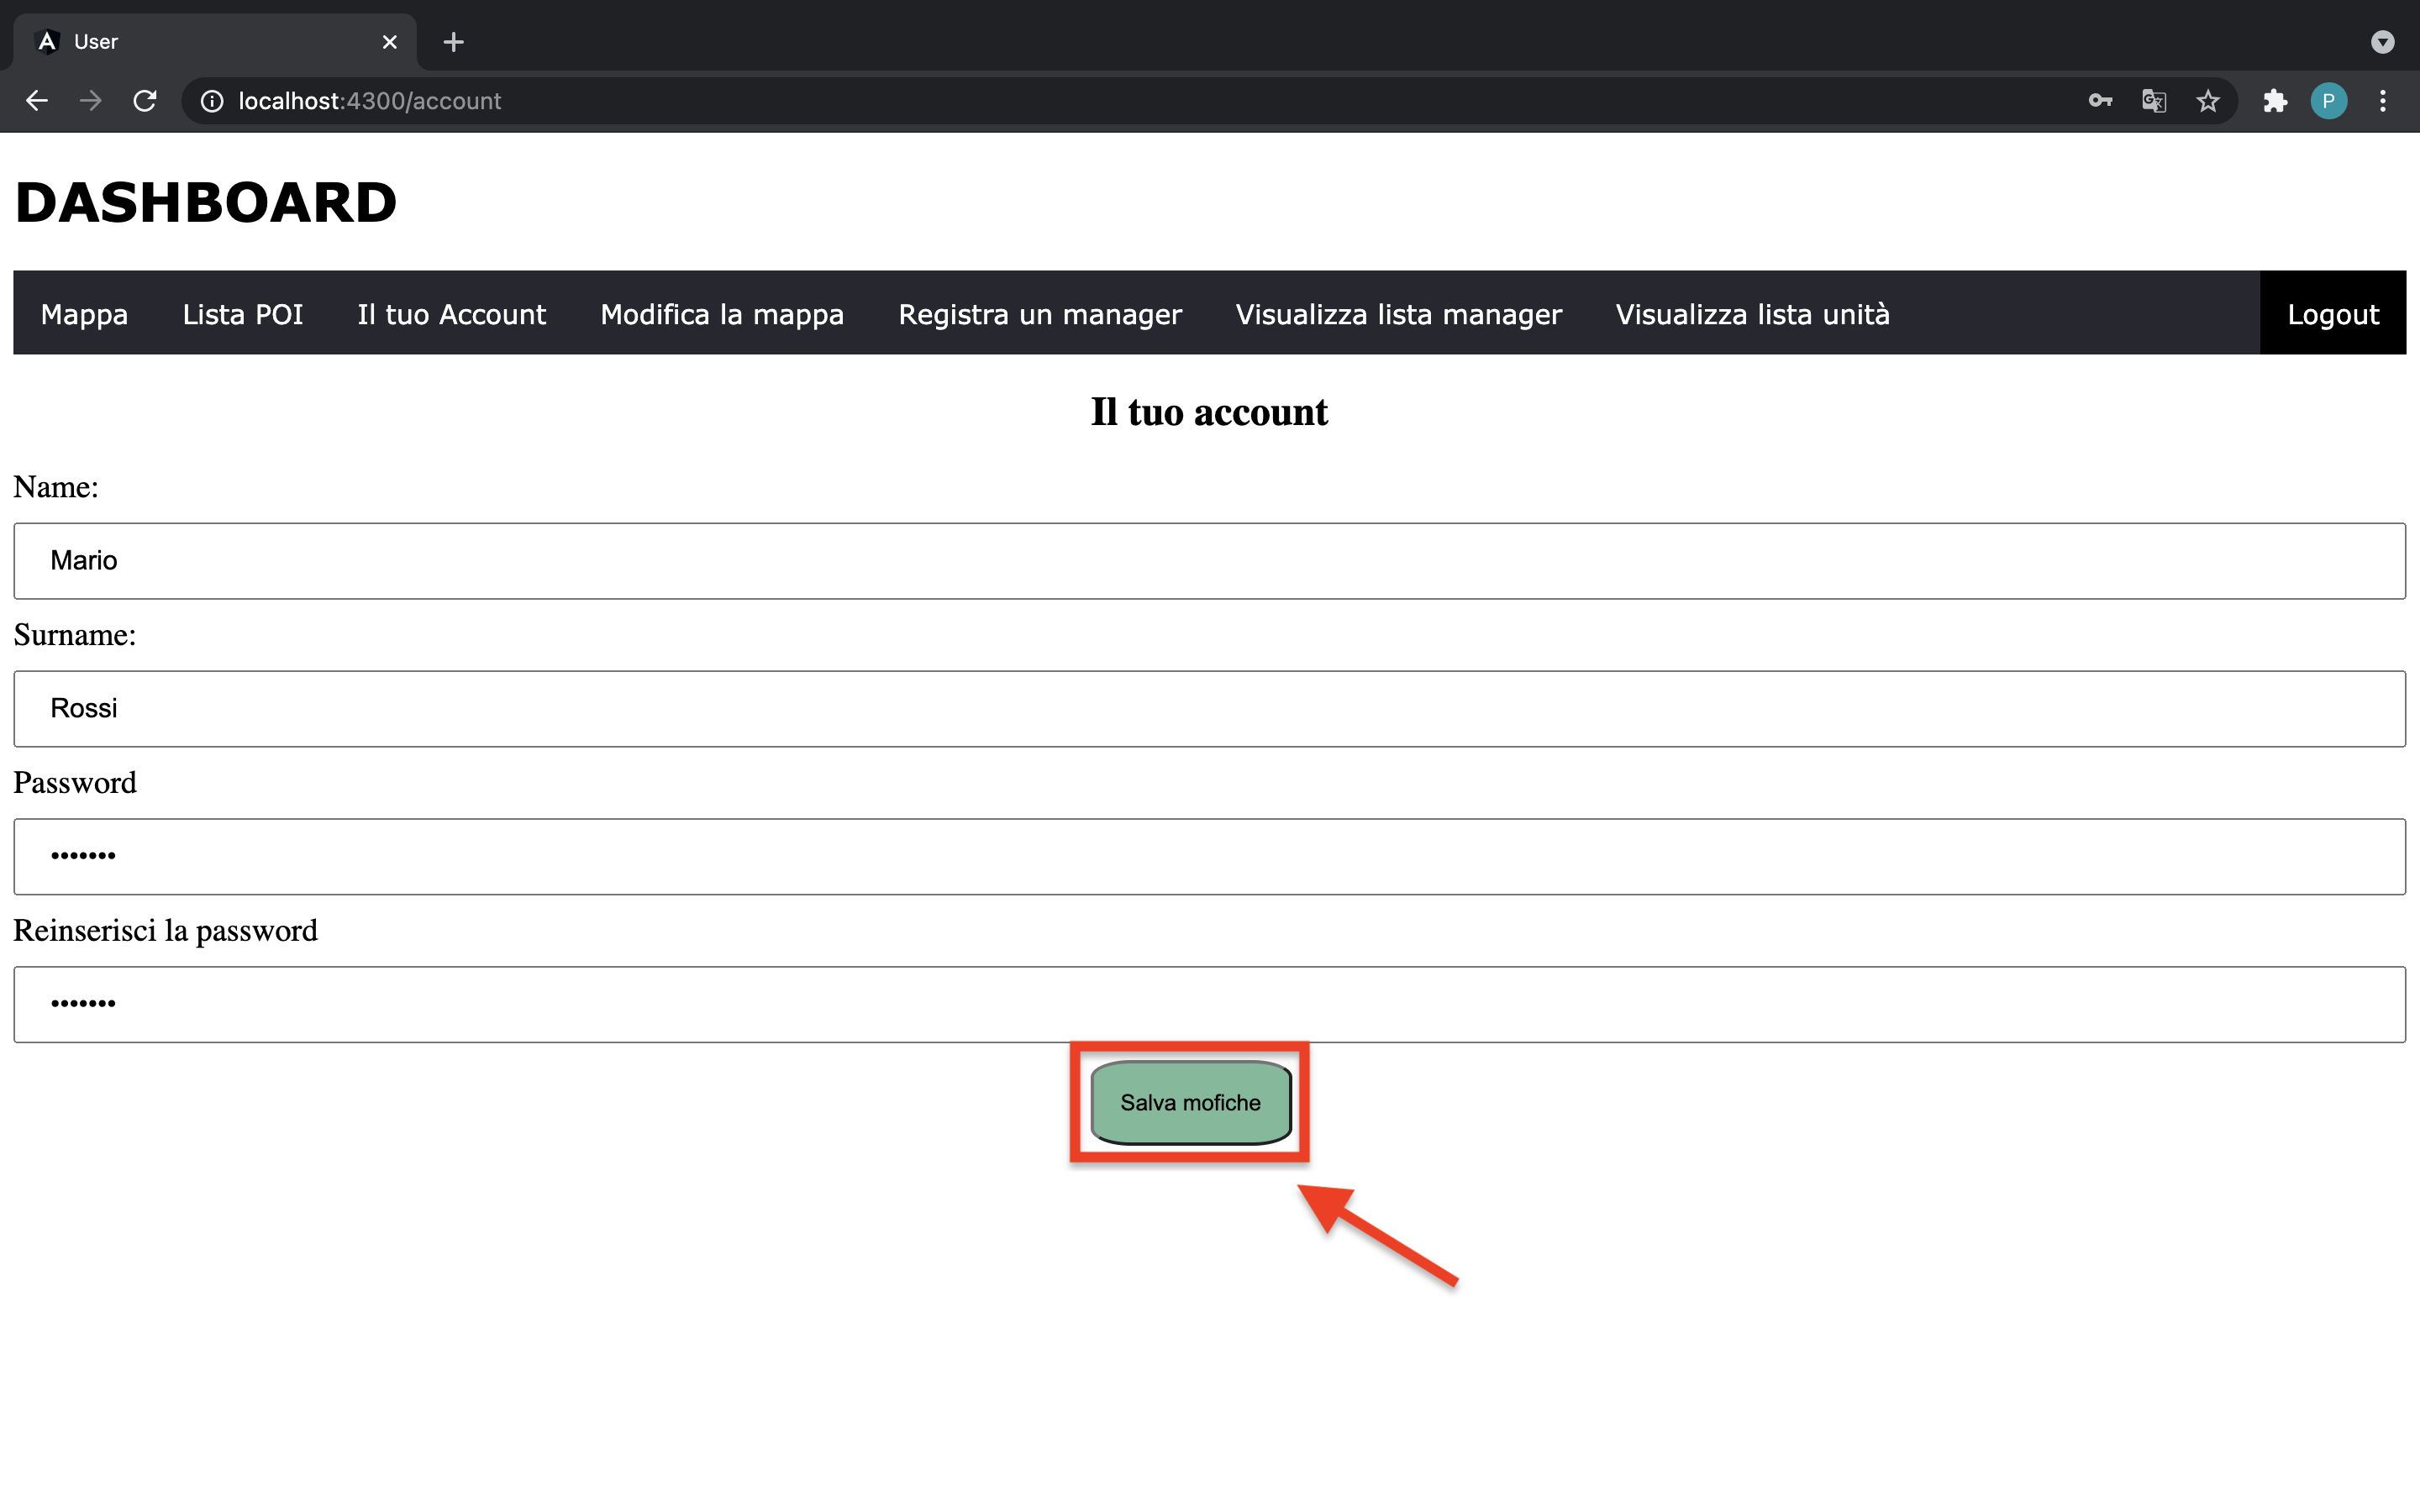
\includegraphics[scale=0.12]{res/images/account_user.png}
        \caption{Istantanea dello schermo di modifica del proprio profilo}
    \end{figure}
    \item Se si intende cambiare la Password, l'inserimento nei due campi deve coincidere altrimenti si visualizzerà un errore.
    \begin{figure}[H]
        \centering
        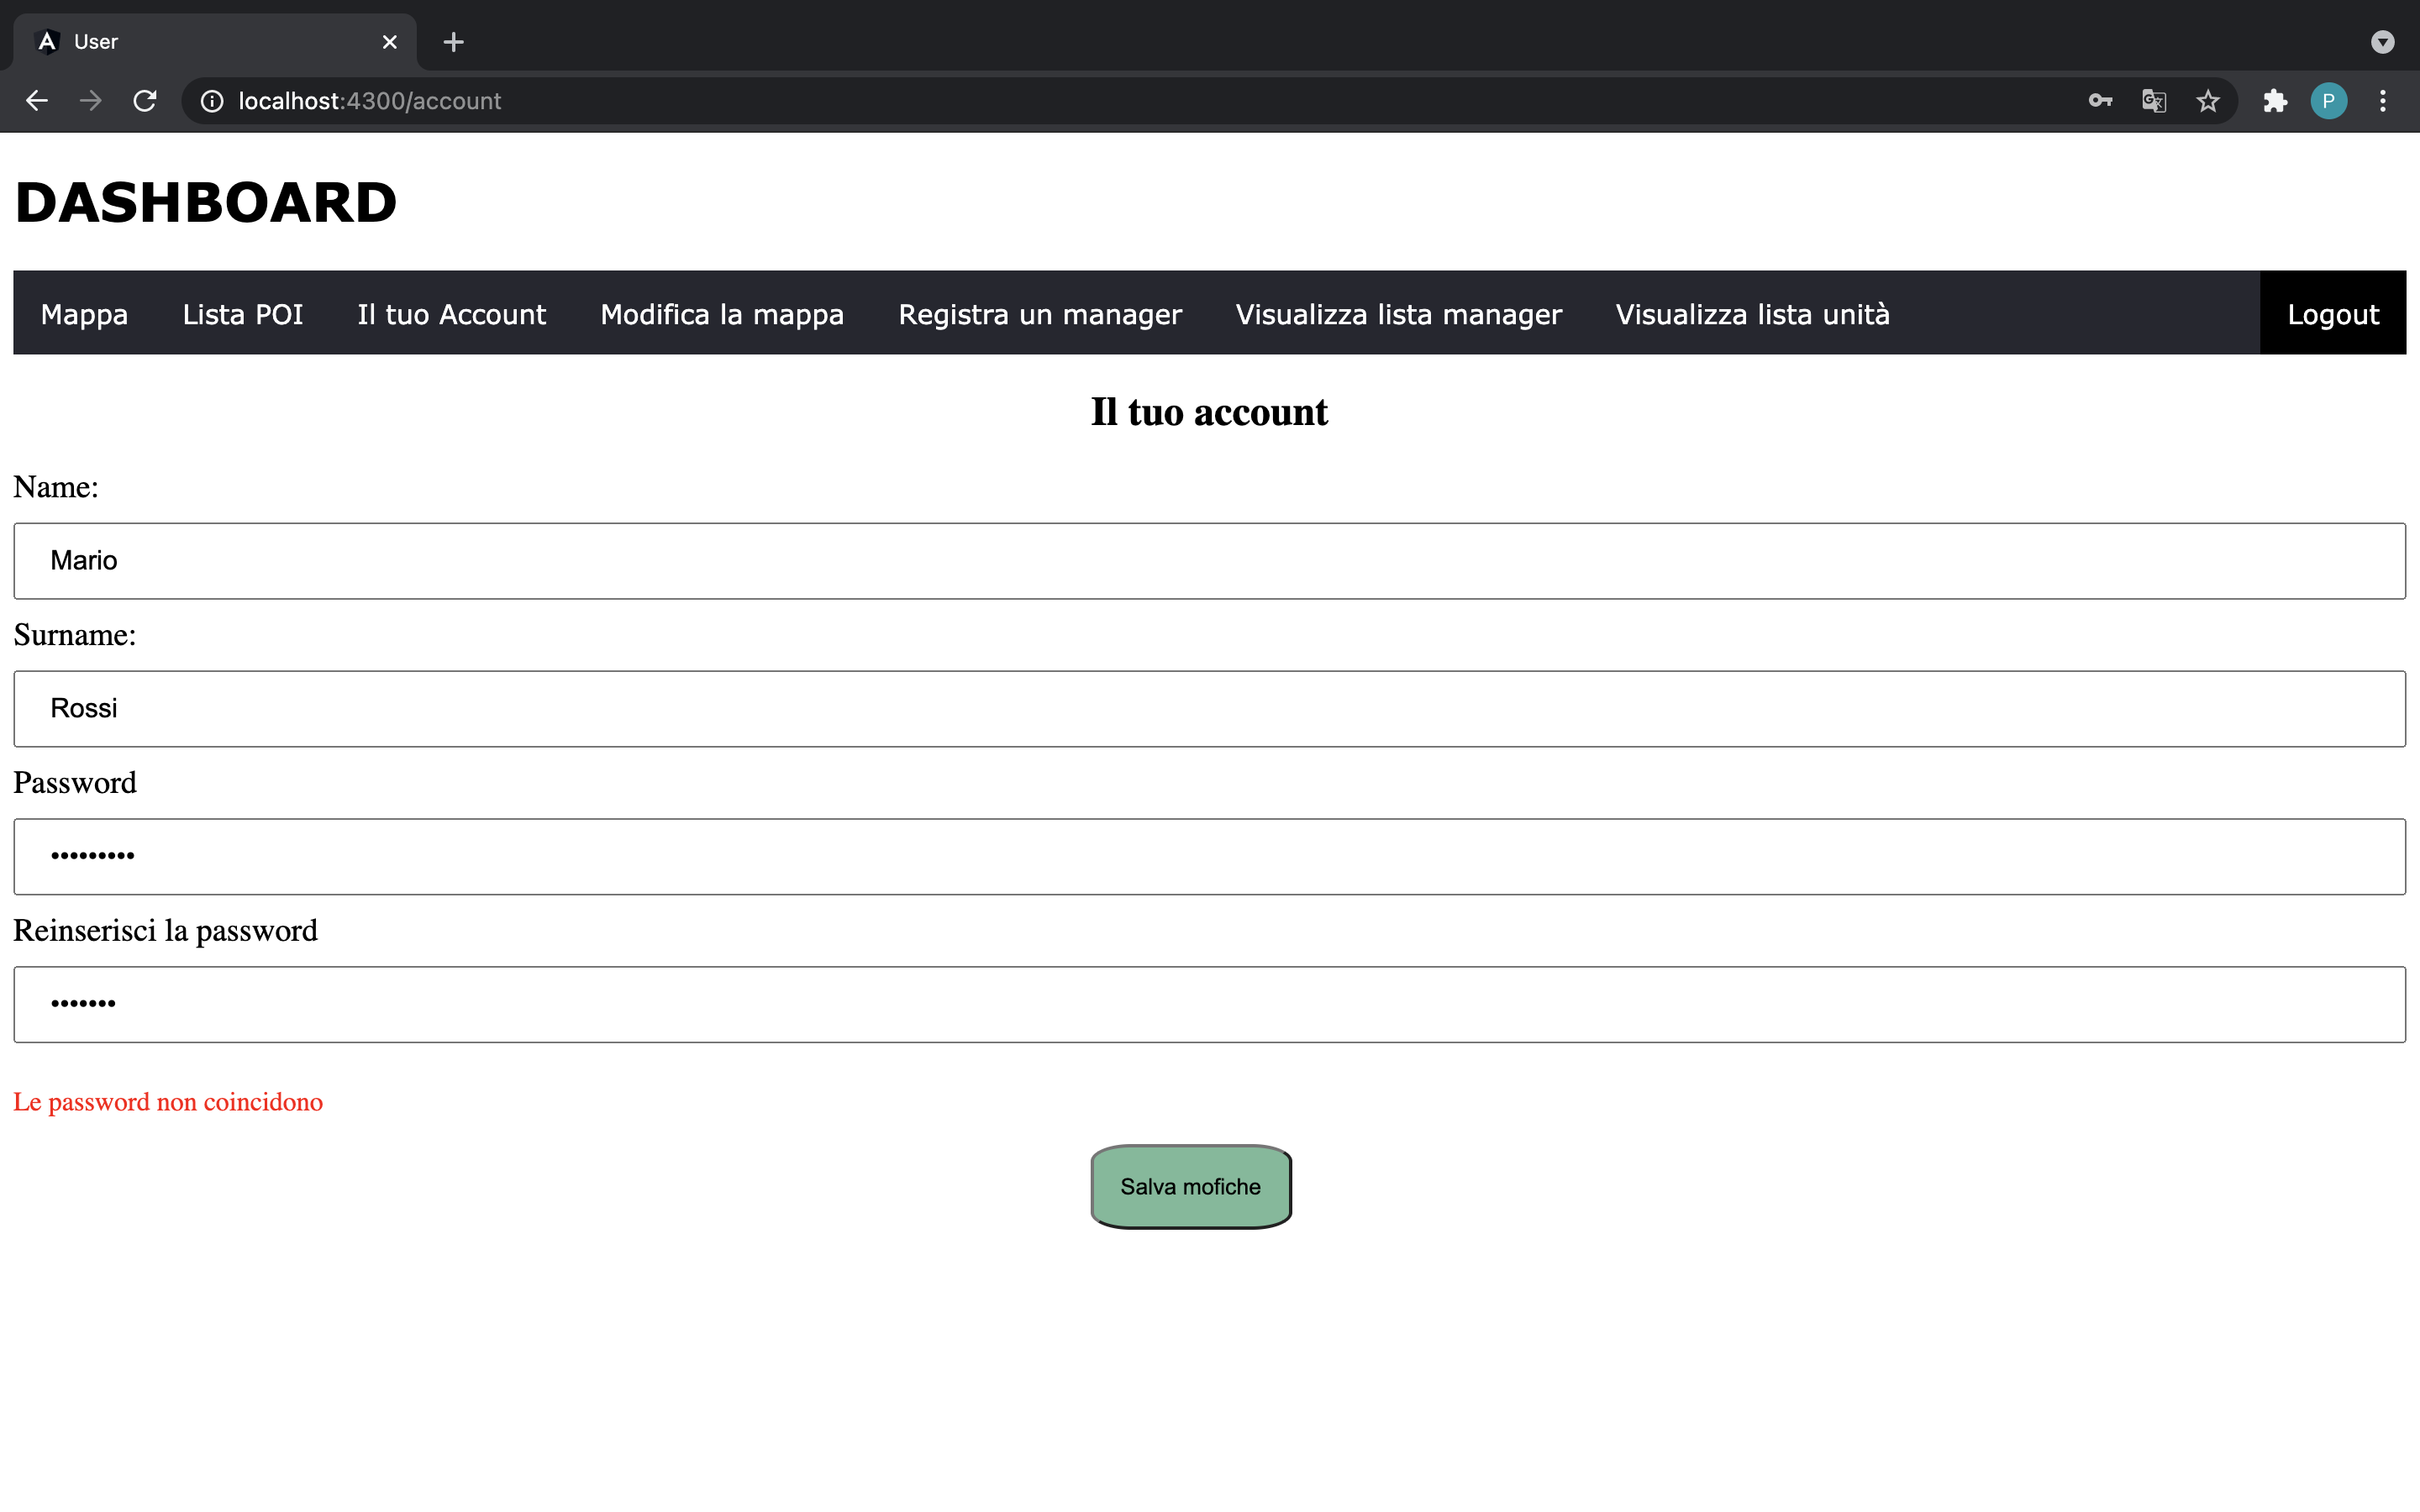
\includegraphics[scale=0.12]{res/images/account_errore.png}
        \caption{Istantanea dello schermo di modifica della password con messaggio d'errore}
    \end{figure}
\end{itemize}


\subsection{Registrazione di un nuovo utente}
\begin{itemize}
    \item Dopo l'autenticazione, tramite il menù selezionare il pulsante "Registra un manager";
    \begin{figure}[H]
        \centering
        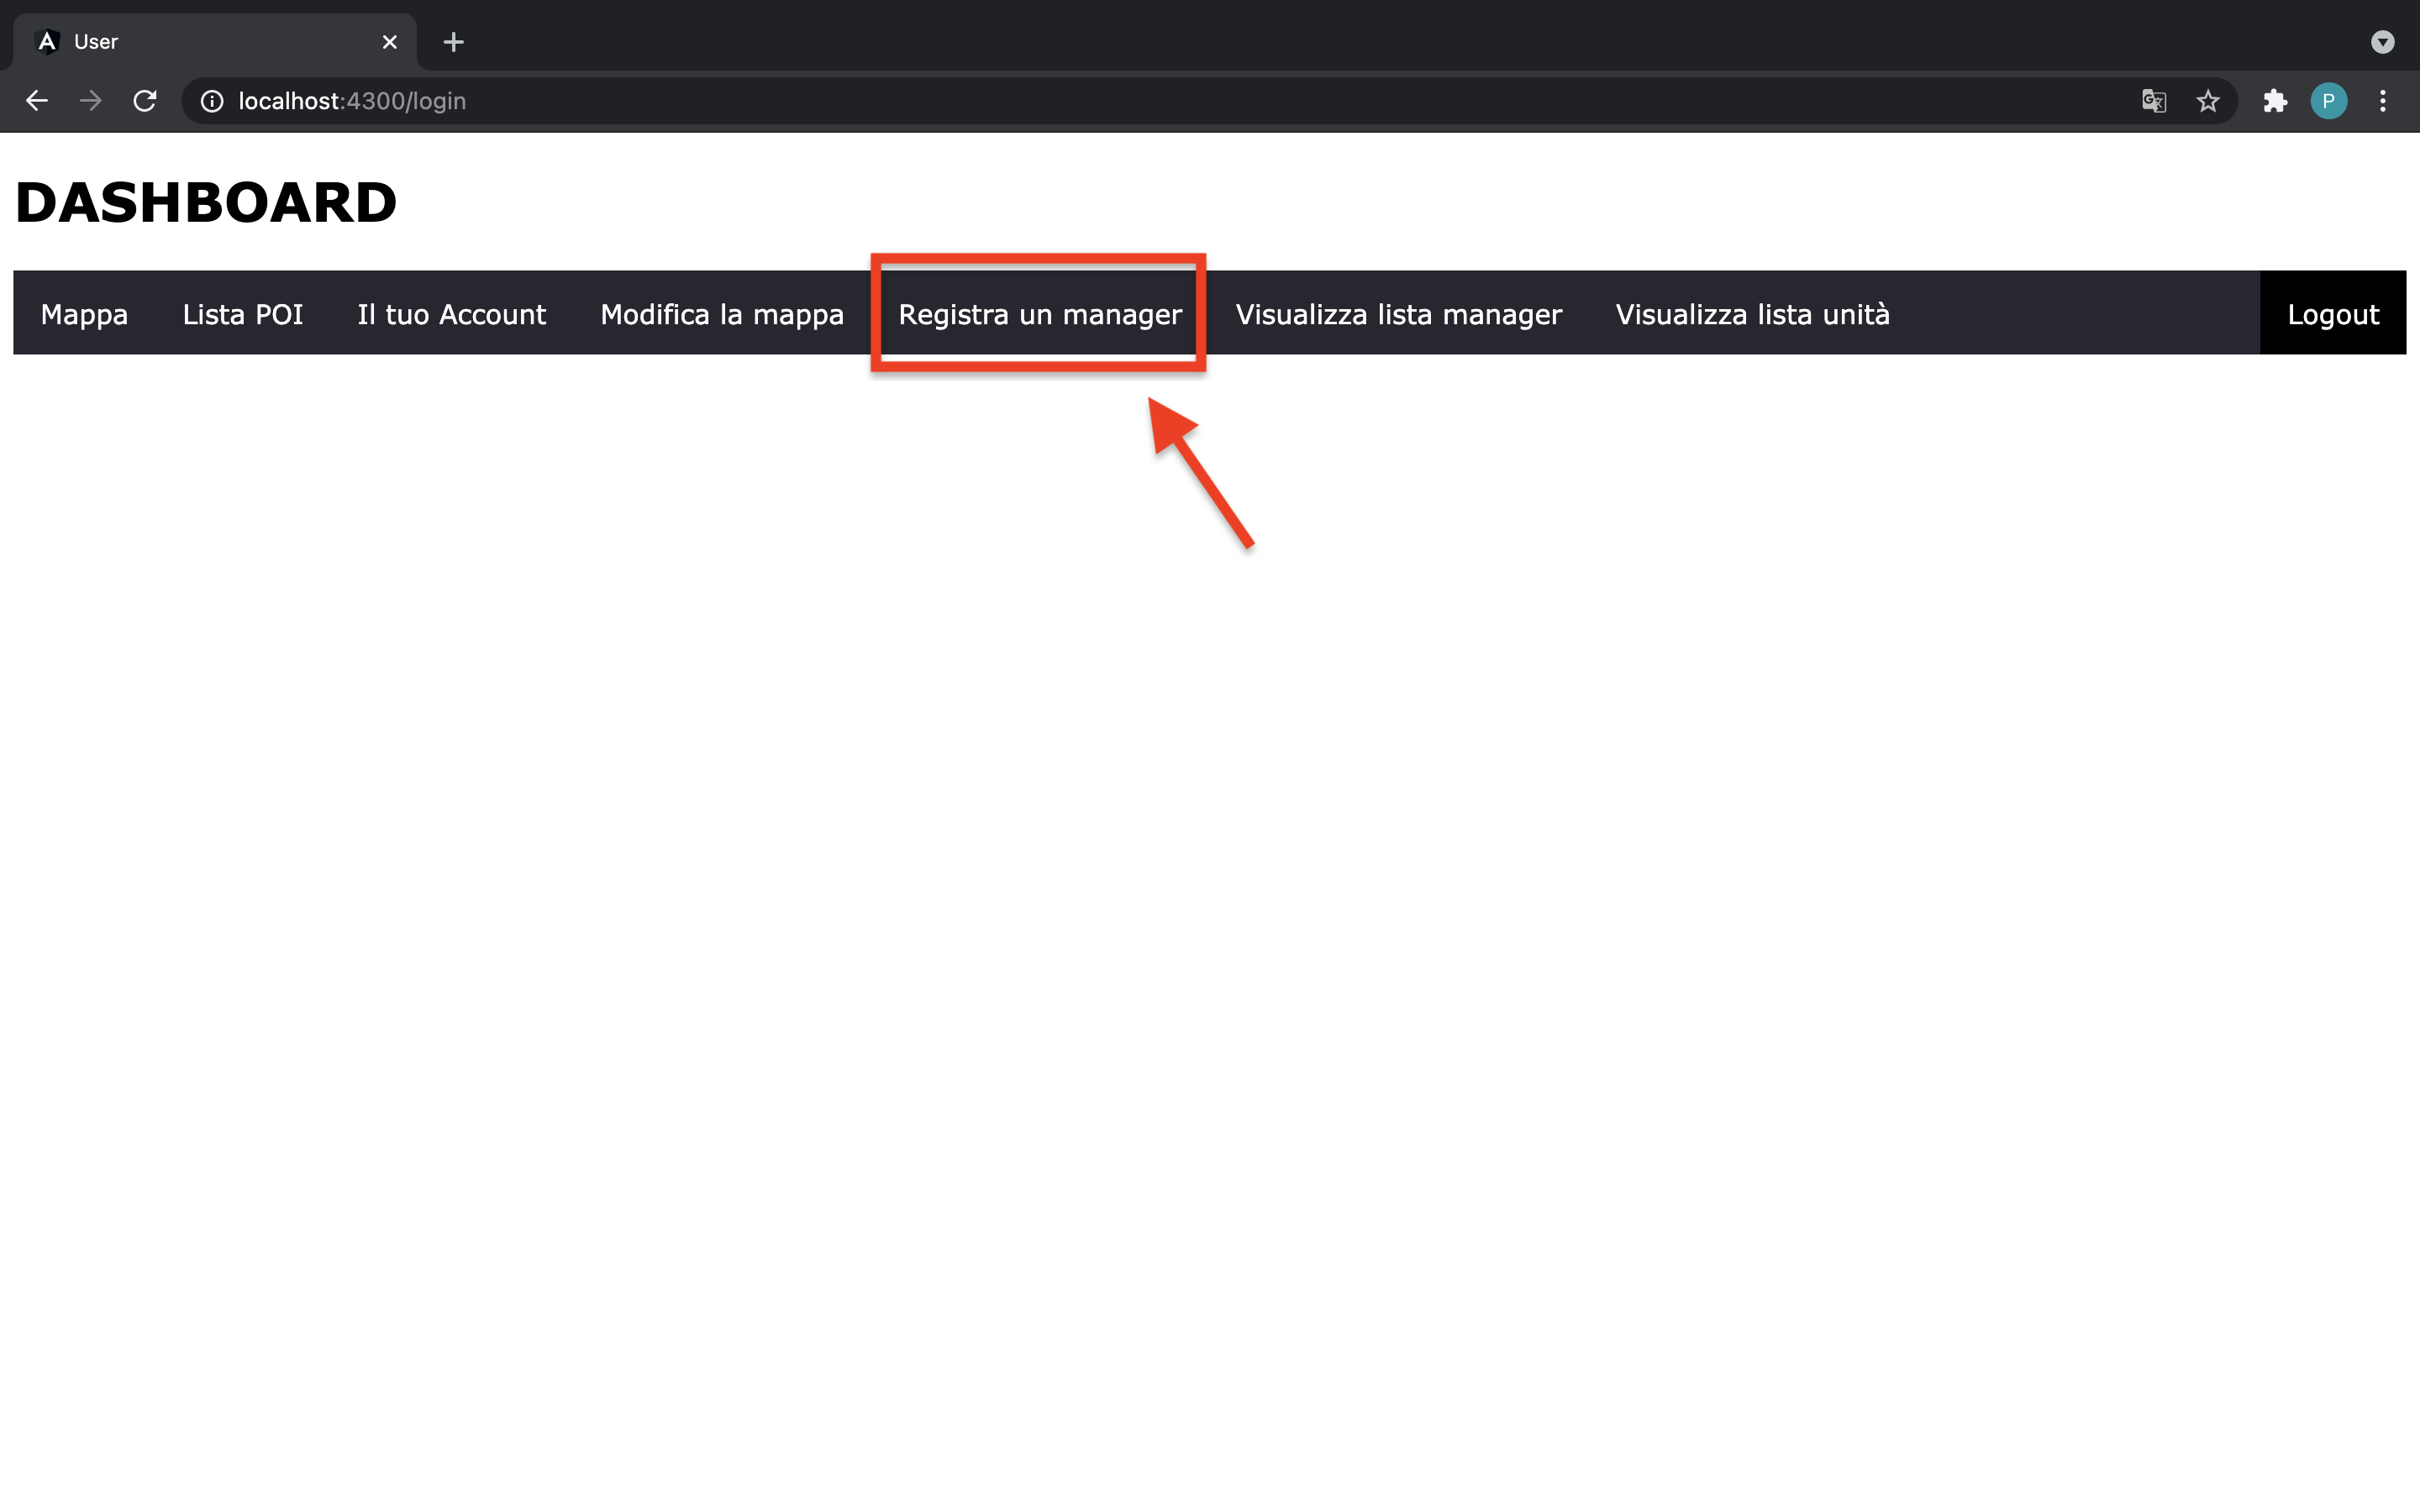
\includegraphics[scale=0.12]{res/images/dashboard4.png}
        \caption{Istantanea dello schermo con indicazione per registrare un nuovo utente}
    \end{figure}
    \item si viene indirizzati alla pagina con i campi da compilare: Nome e Cognome;
\end{itemize}
\begin{figure}[H]
    \centering
    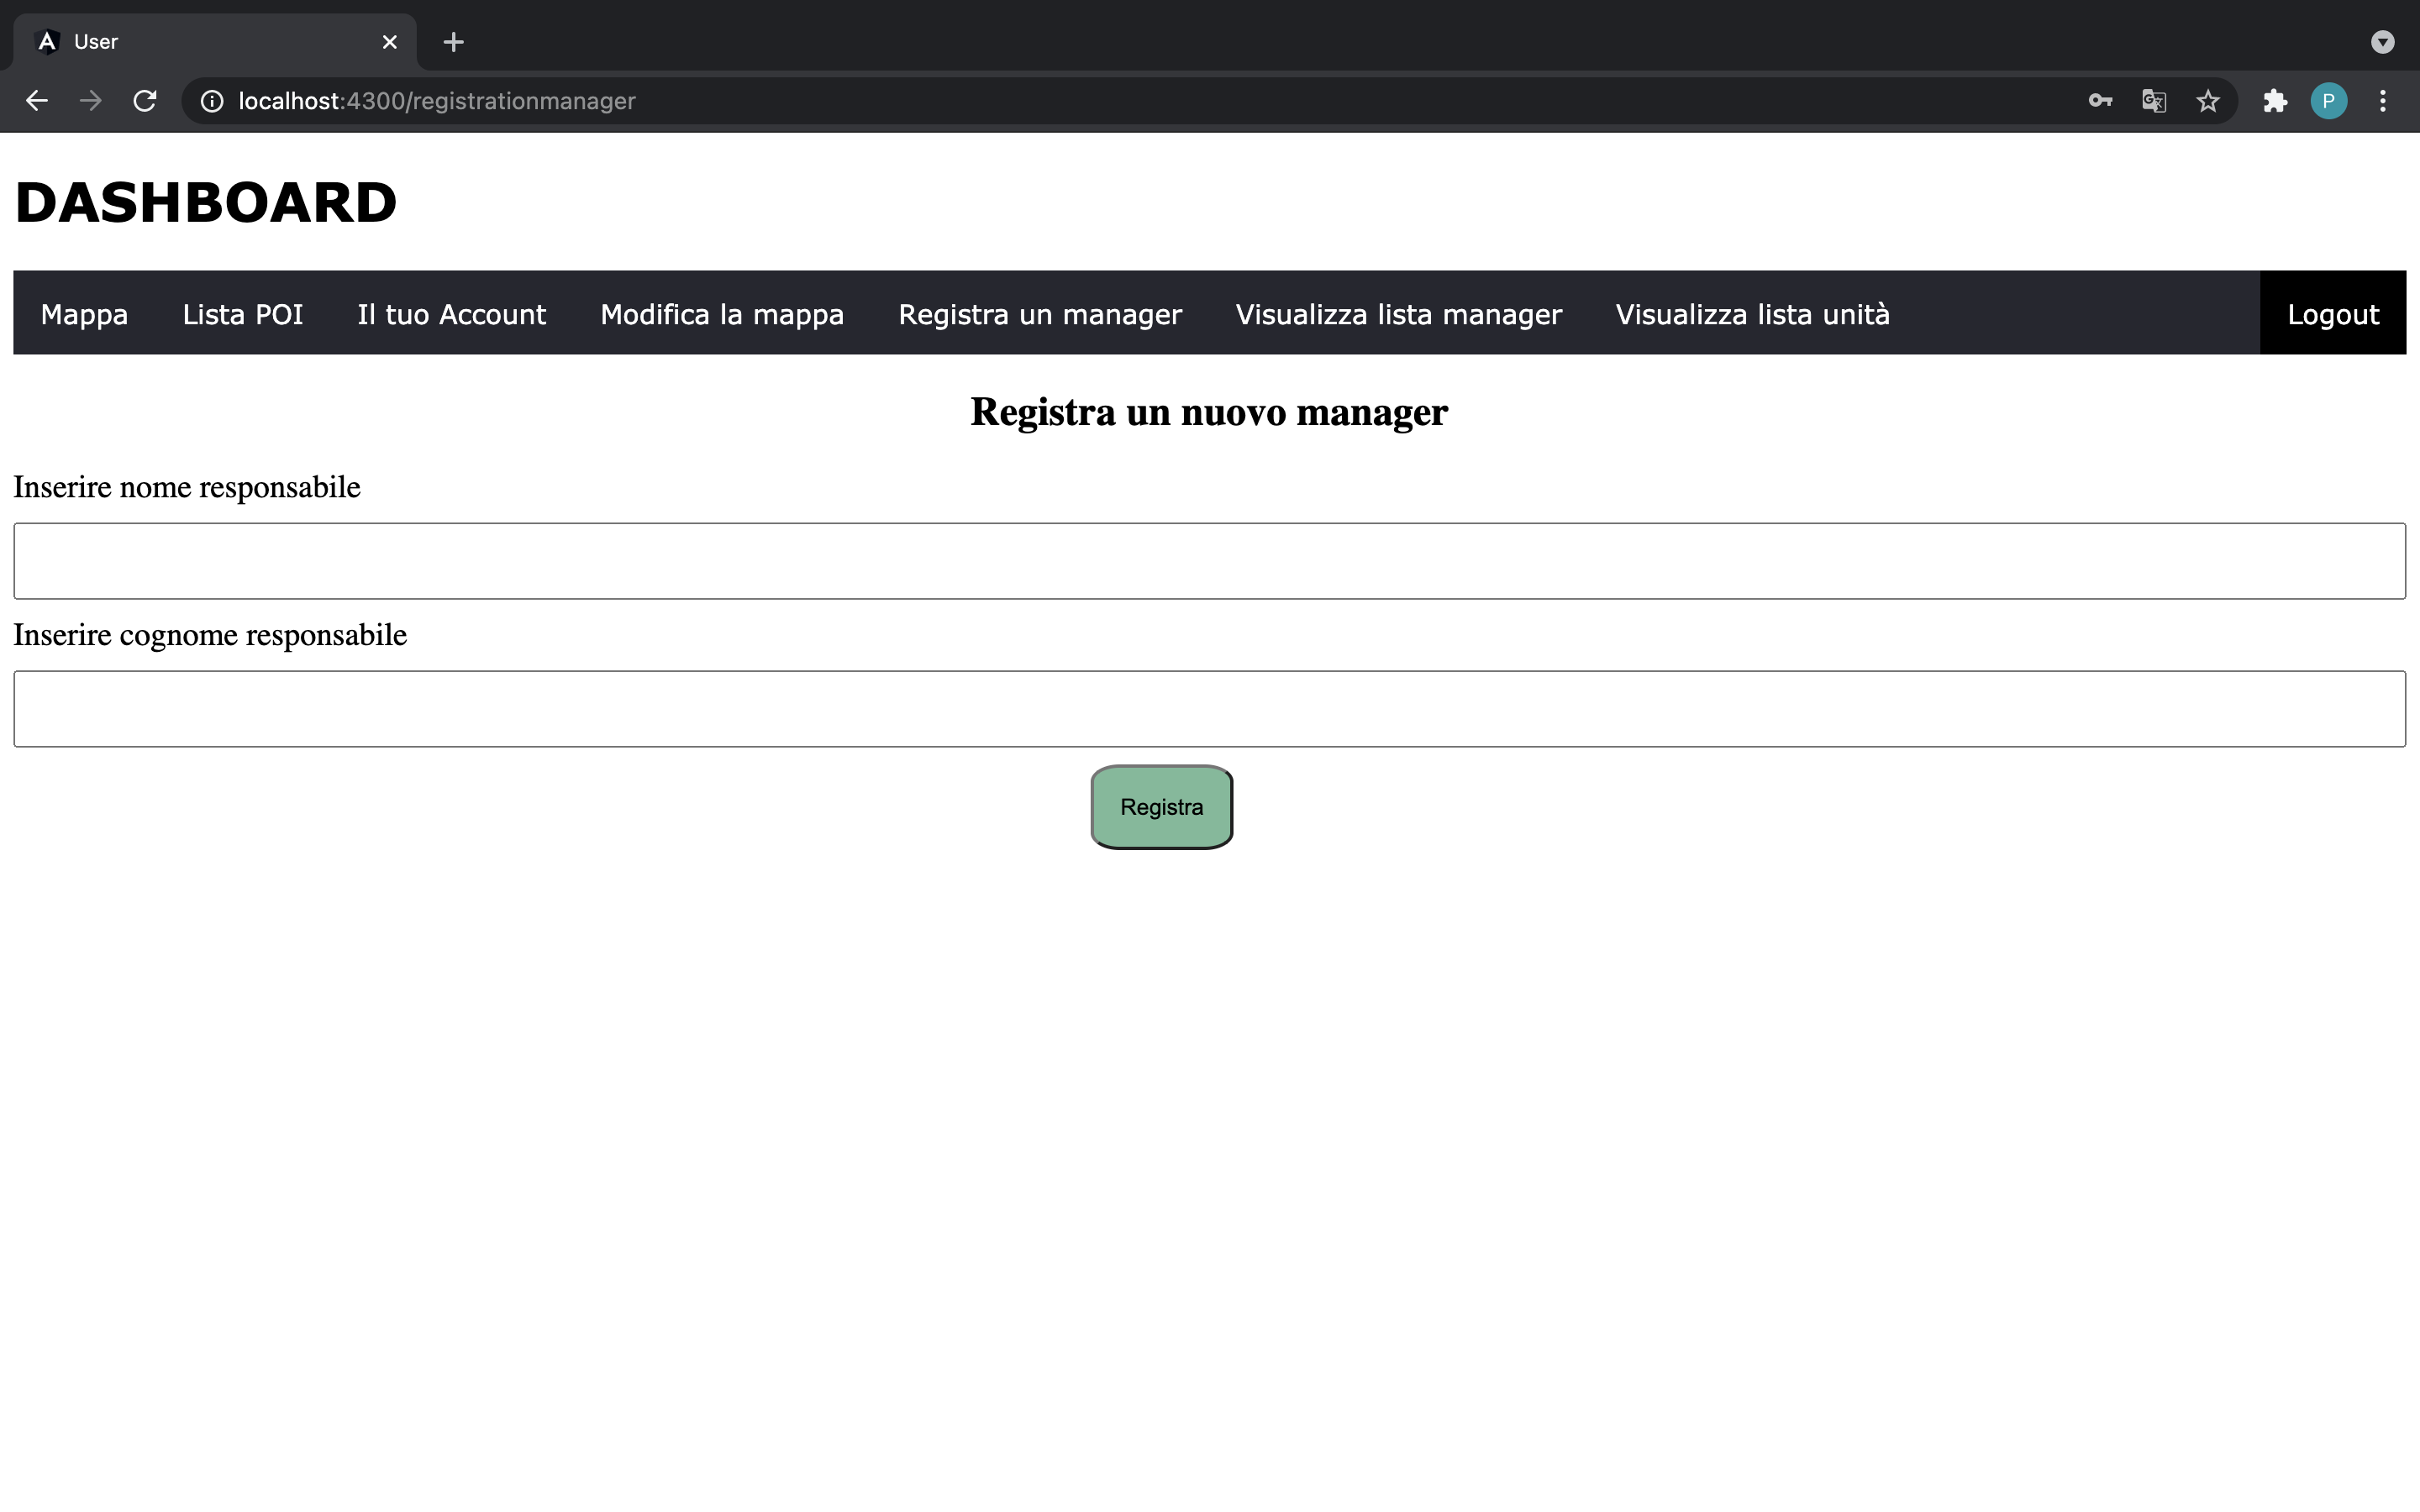
\includegraphics[scale=0.12]{res/images/newmanager.png}
    \caption{Istantanea dello schermo registrazione manager}
\end{figure}
\begin{itemize}
    \item inserire i dati e premere sul pulsante "Registra";
    \begin{figure}[H]
        \centering
        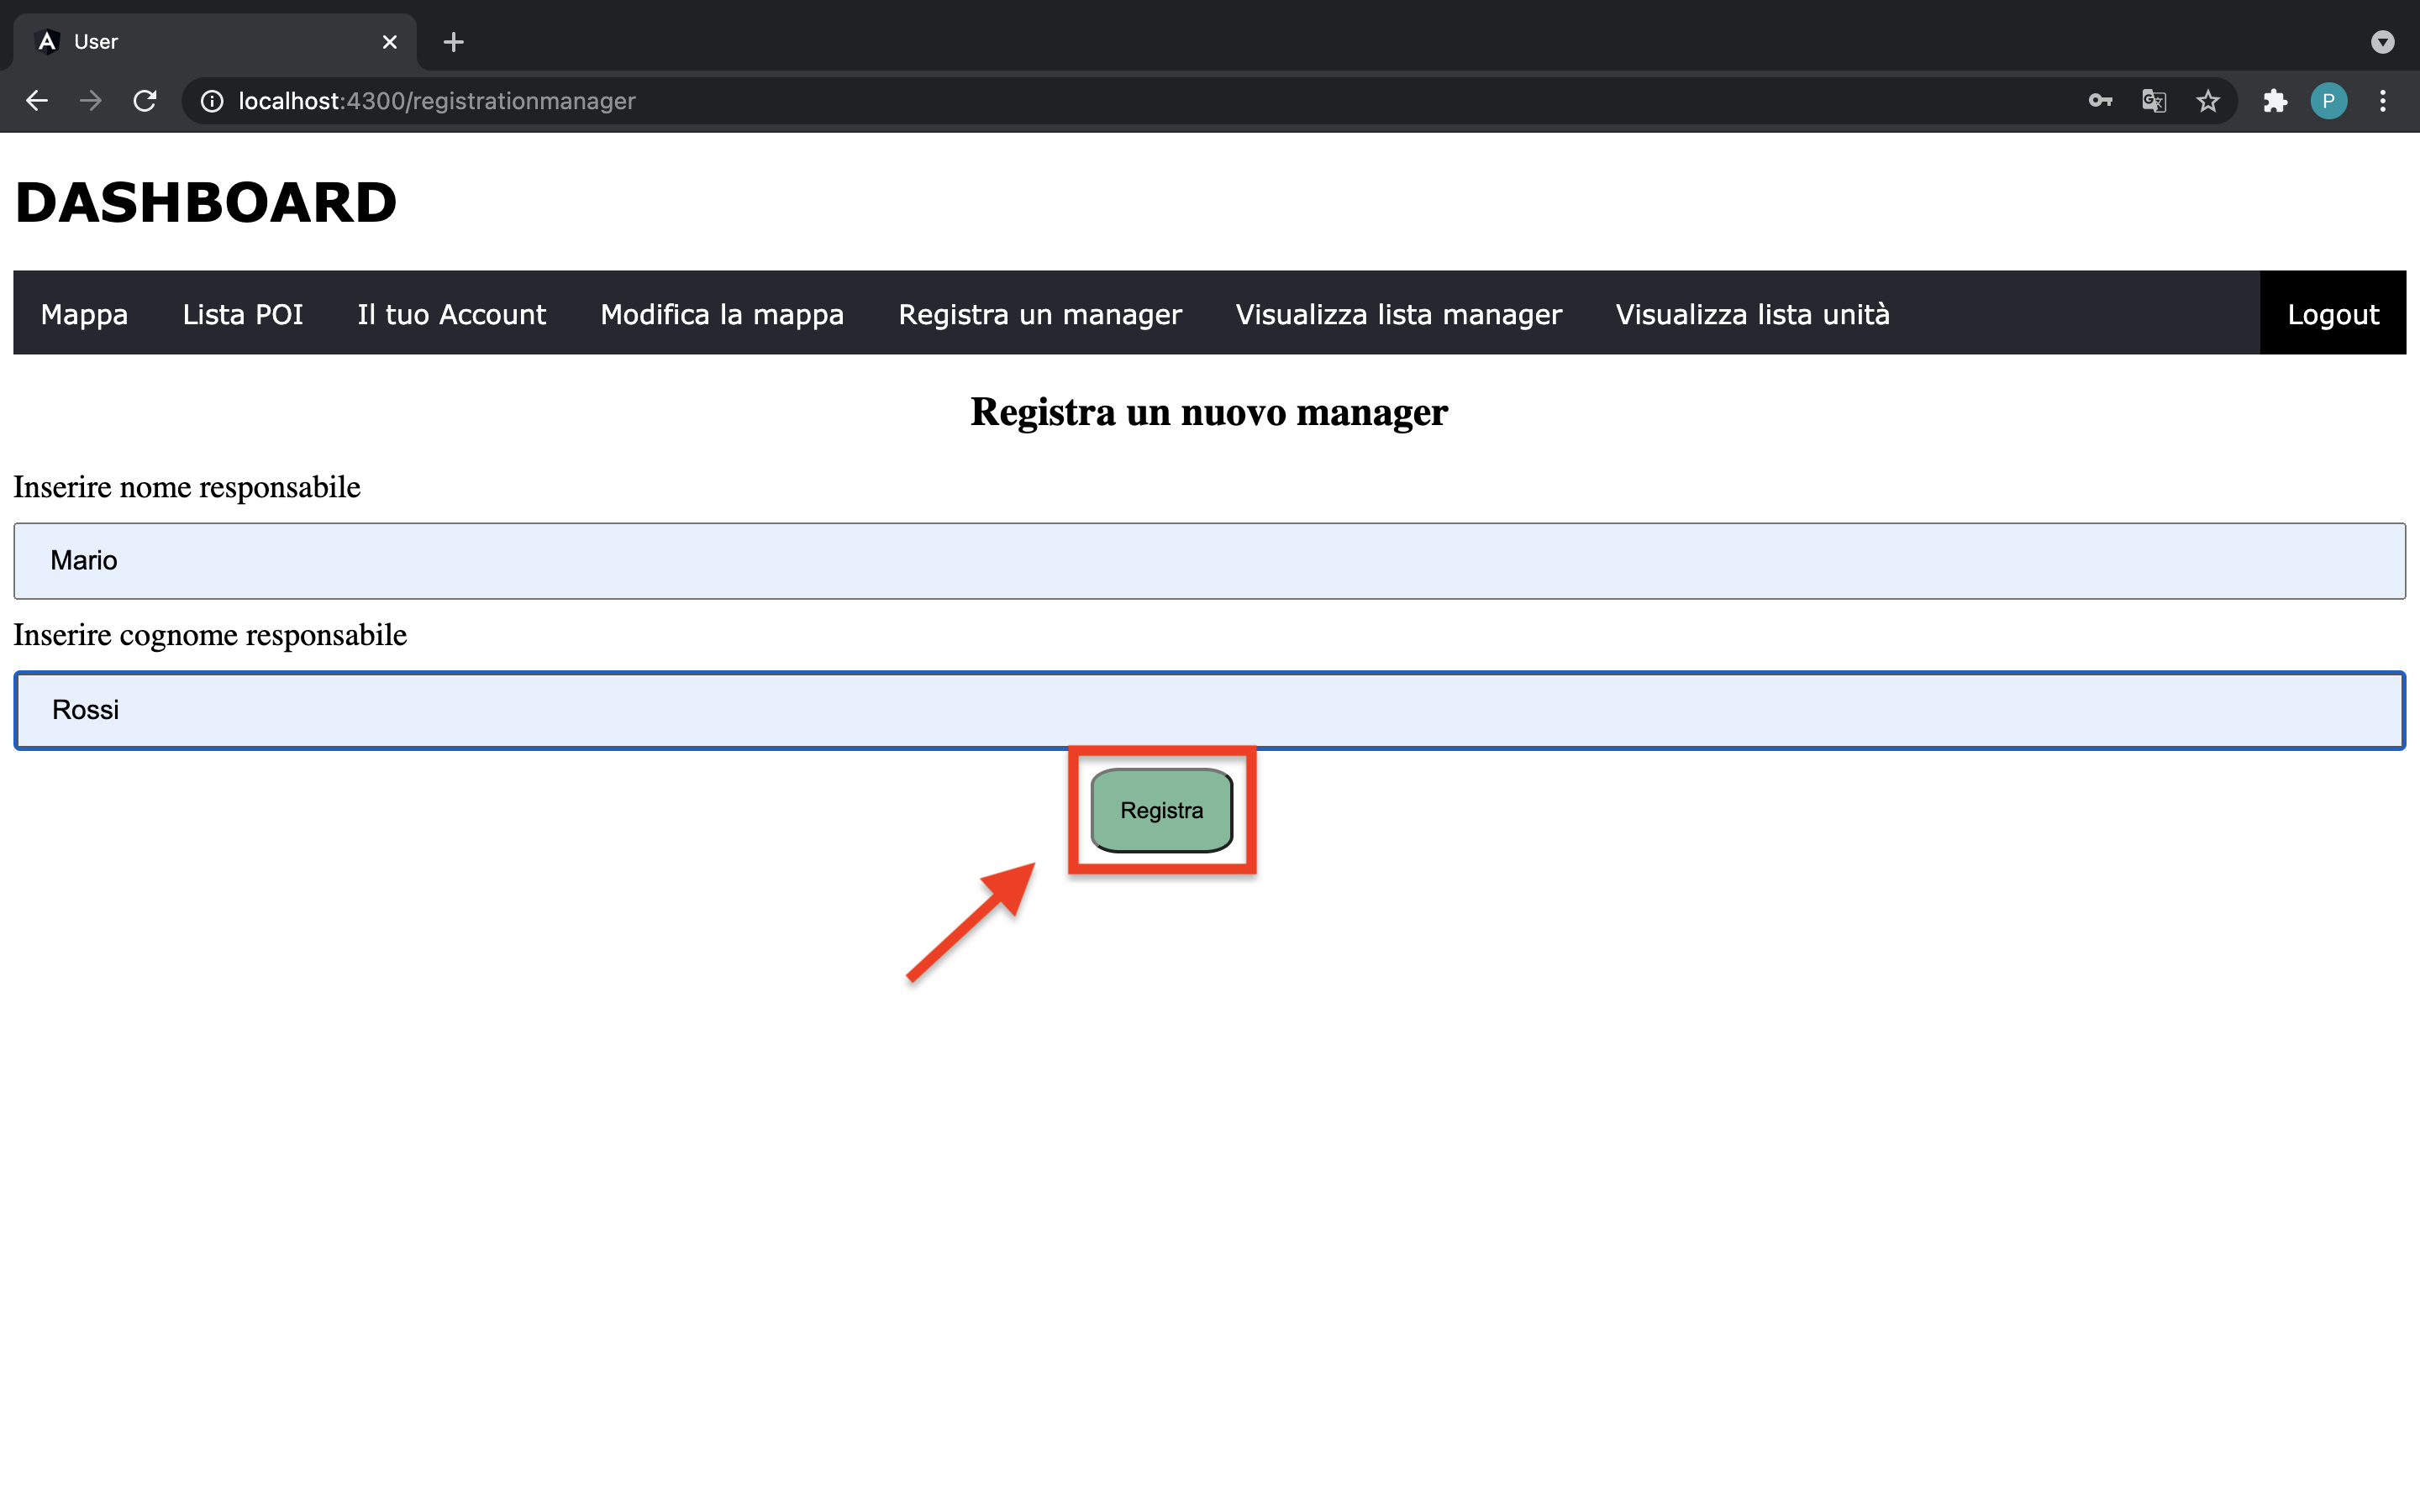
\includegraphics[scale=0.12]{res/images/newmanager_2.png}
        \caption{Istantanea dello schermo registrazione manager 2}
    \end{figure}
    \item viene visualizzato a video la password e il codice identificativo da riferire al nuovo utente per il suo primo accesso.
    \begin{figure}[H]
        \centering
        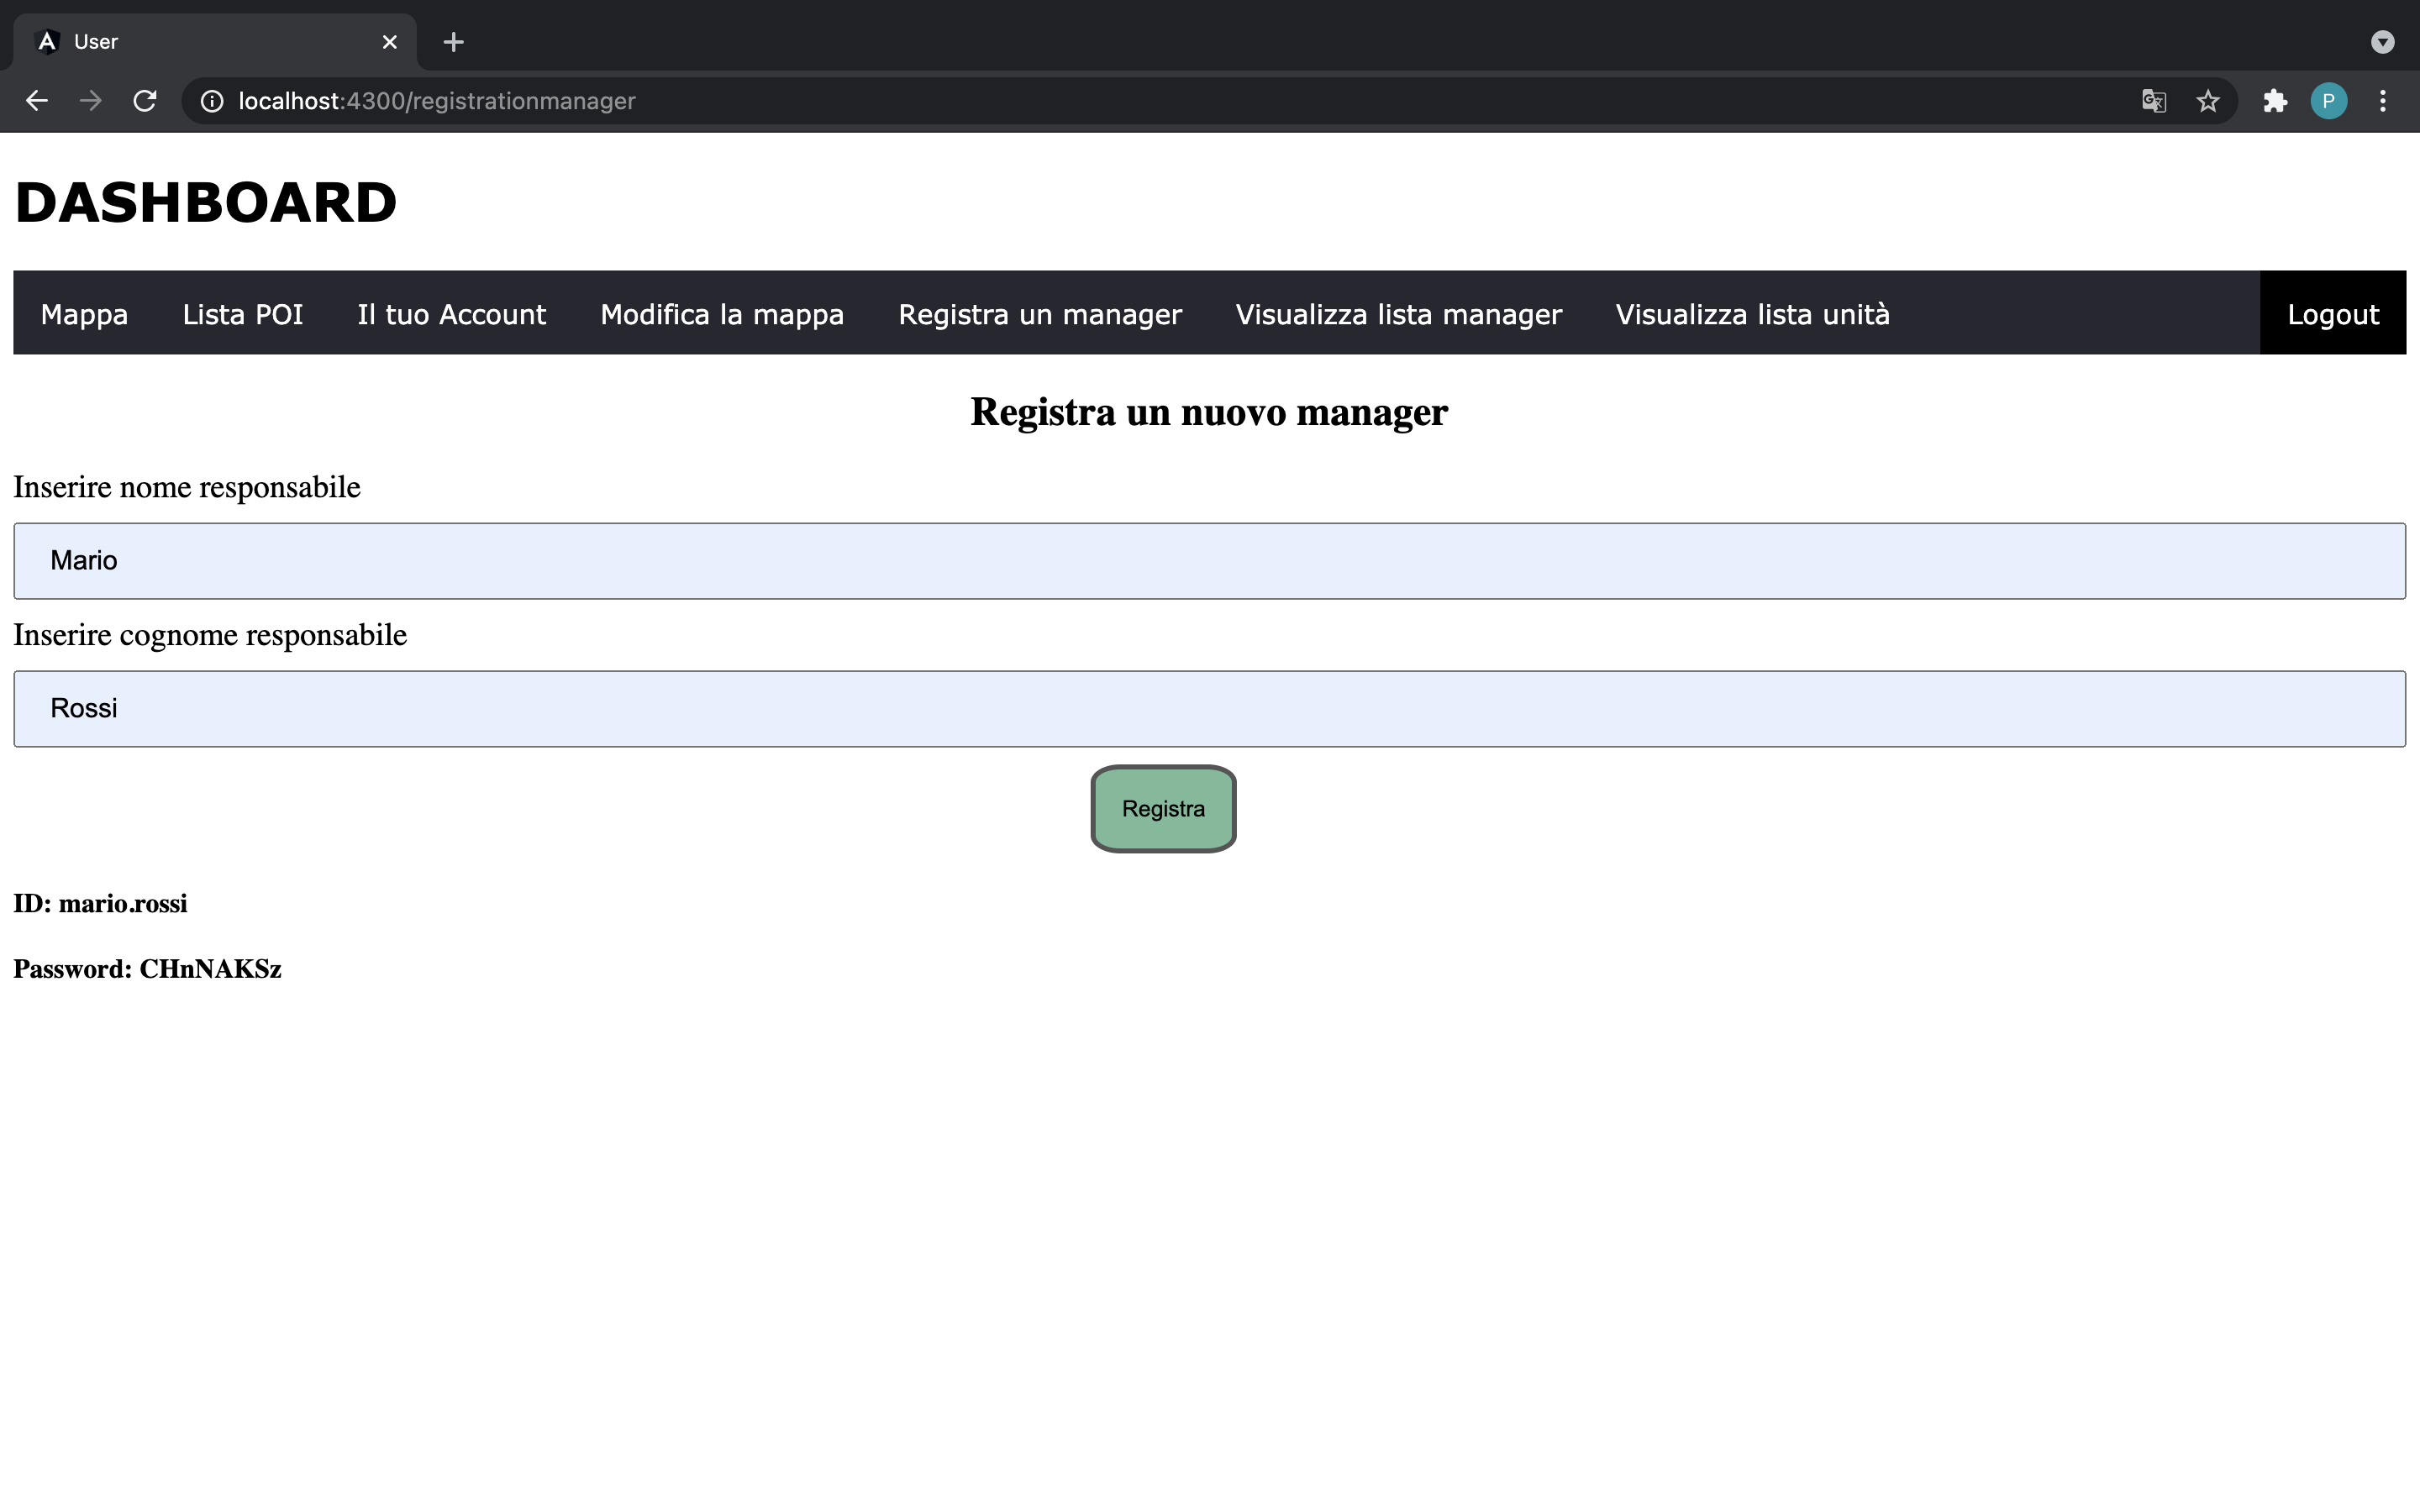
\includegraphics[scale=0.12]{res/images/newmanager3.png}
        \caption{Istantanea dello schermo registrazione manager 3}
    \end{figure}
\end{itemize}




\subsection{Gestione account già presenti}
\begin{itemize}
    \item Dopo l'autenticazione, tramite il menù selezionare il pulsante "Visualizza lista manager";
    \begin{figure}[H]
        \centering
        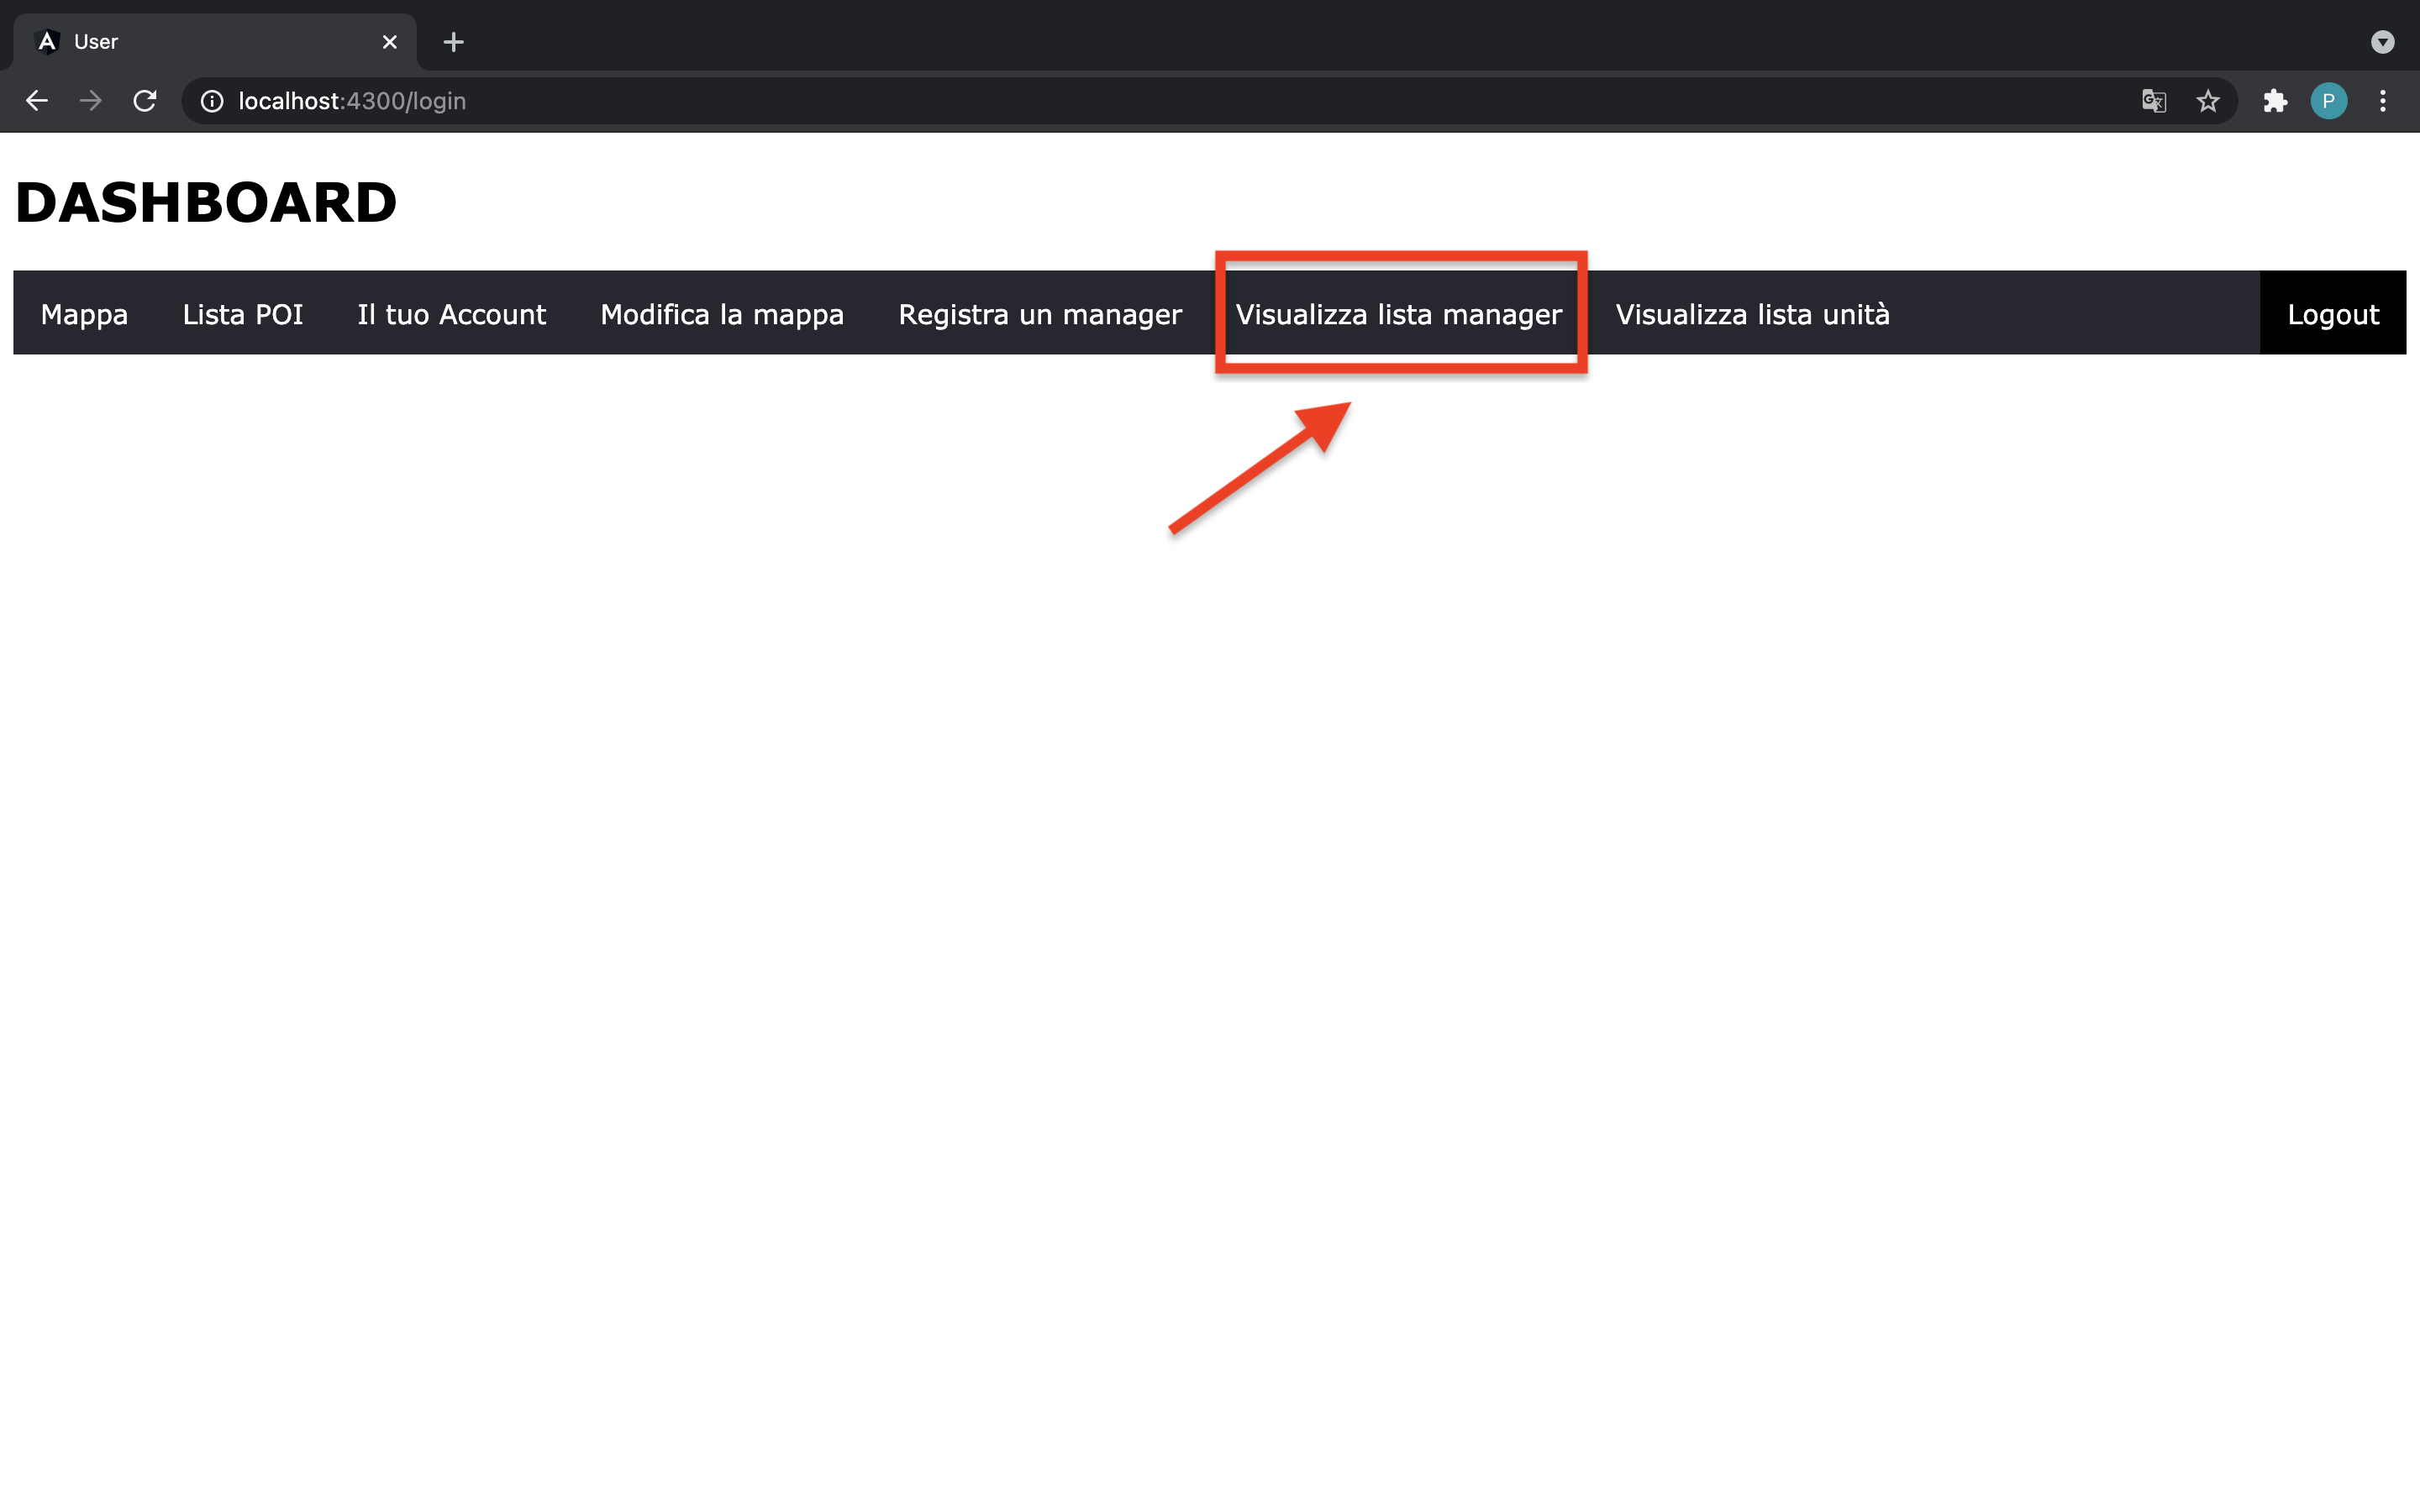
\includegraphics[scale=0.12]{res/images/dashboard5.png}
        \caption{Istantanea dello schermo dashboard con indicazione per la visualizzazione della lista di manager}
    \end{figure}
    \item si viene indirizzati alla pagina con la lista di tutti gli account presenti;
    \item per ogni account è possibile:
        \begin{itemize}
            \item cambiare i campi Nome e Cognome e premere su "Conferma Modifica" per confermare le modifiche;
            \begin{figure}[H]
                \centering
                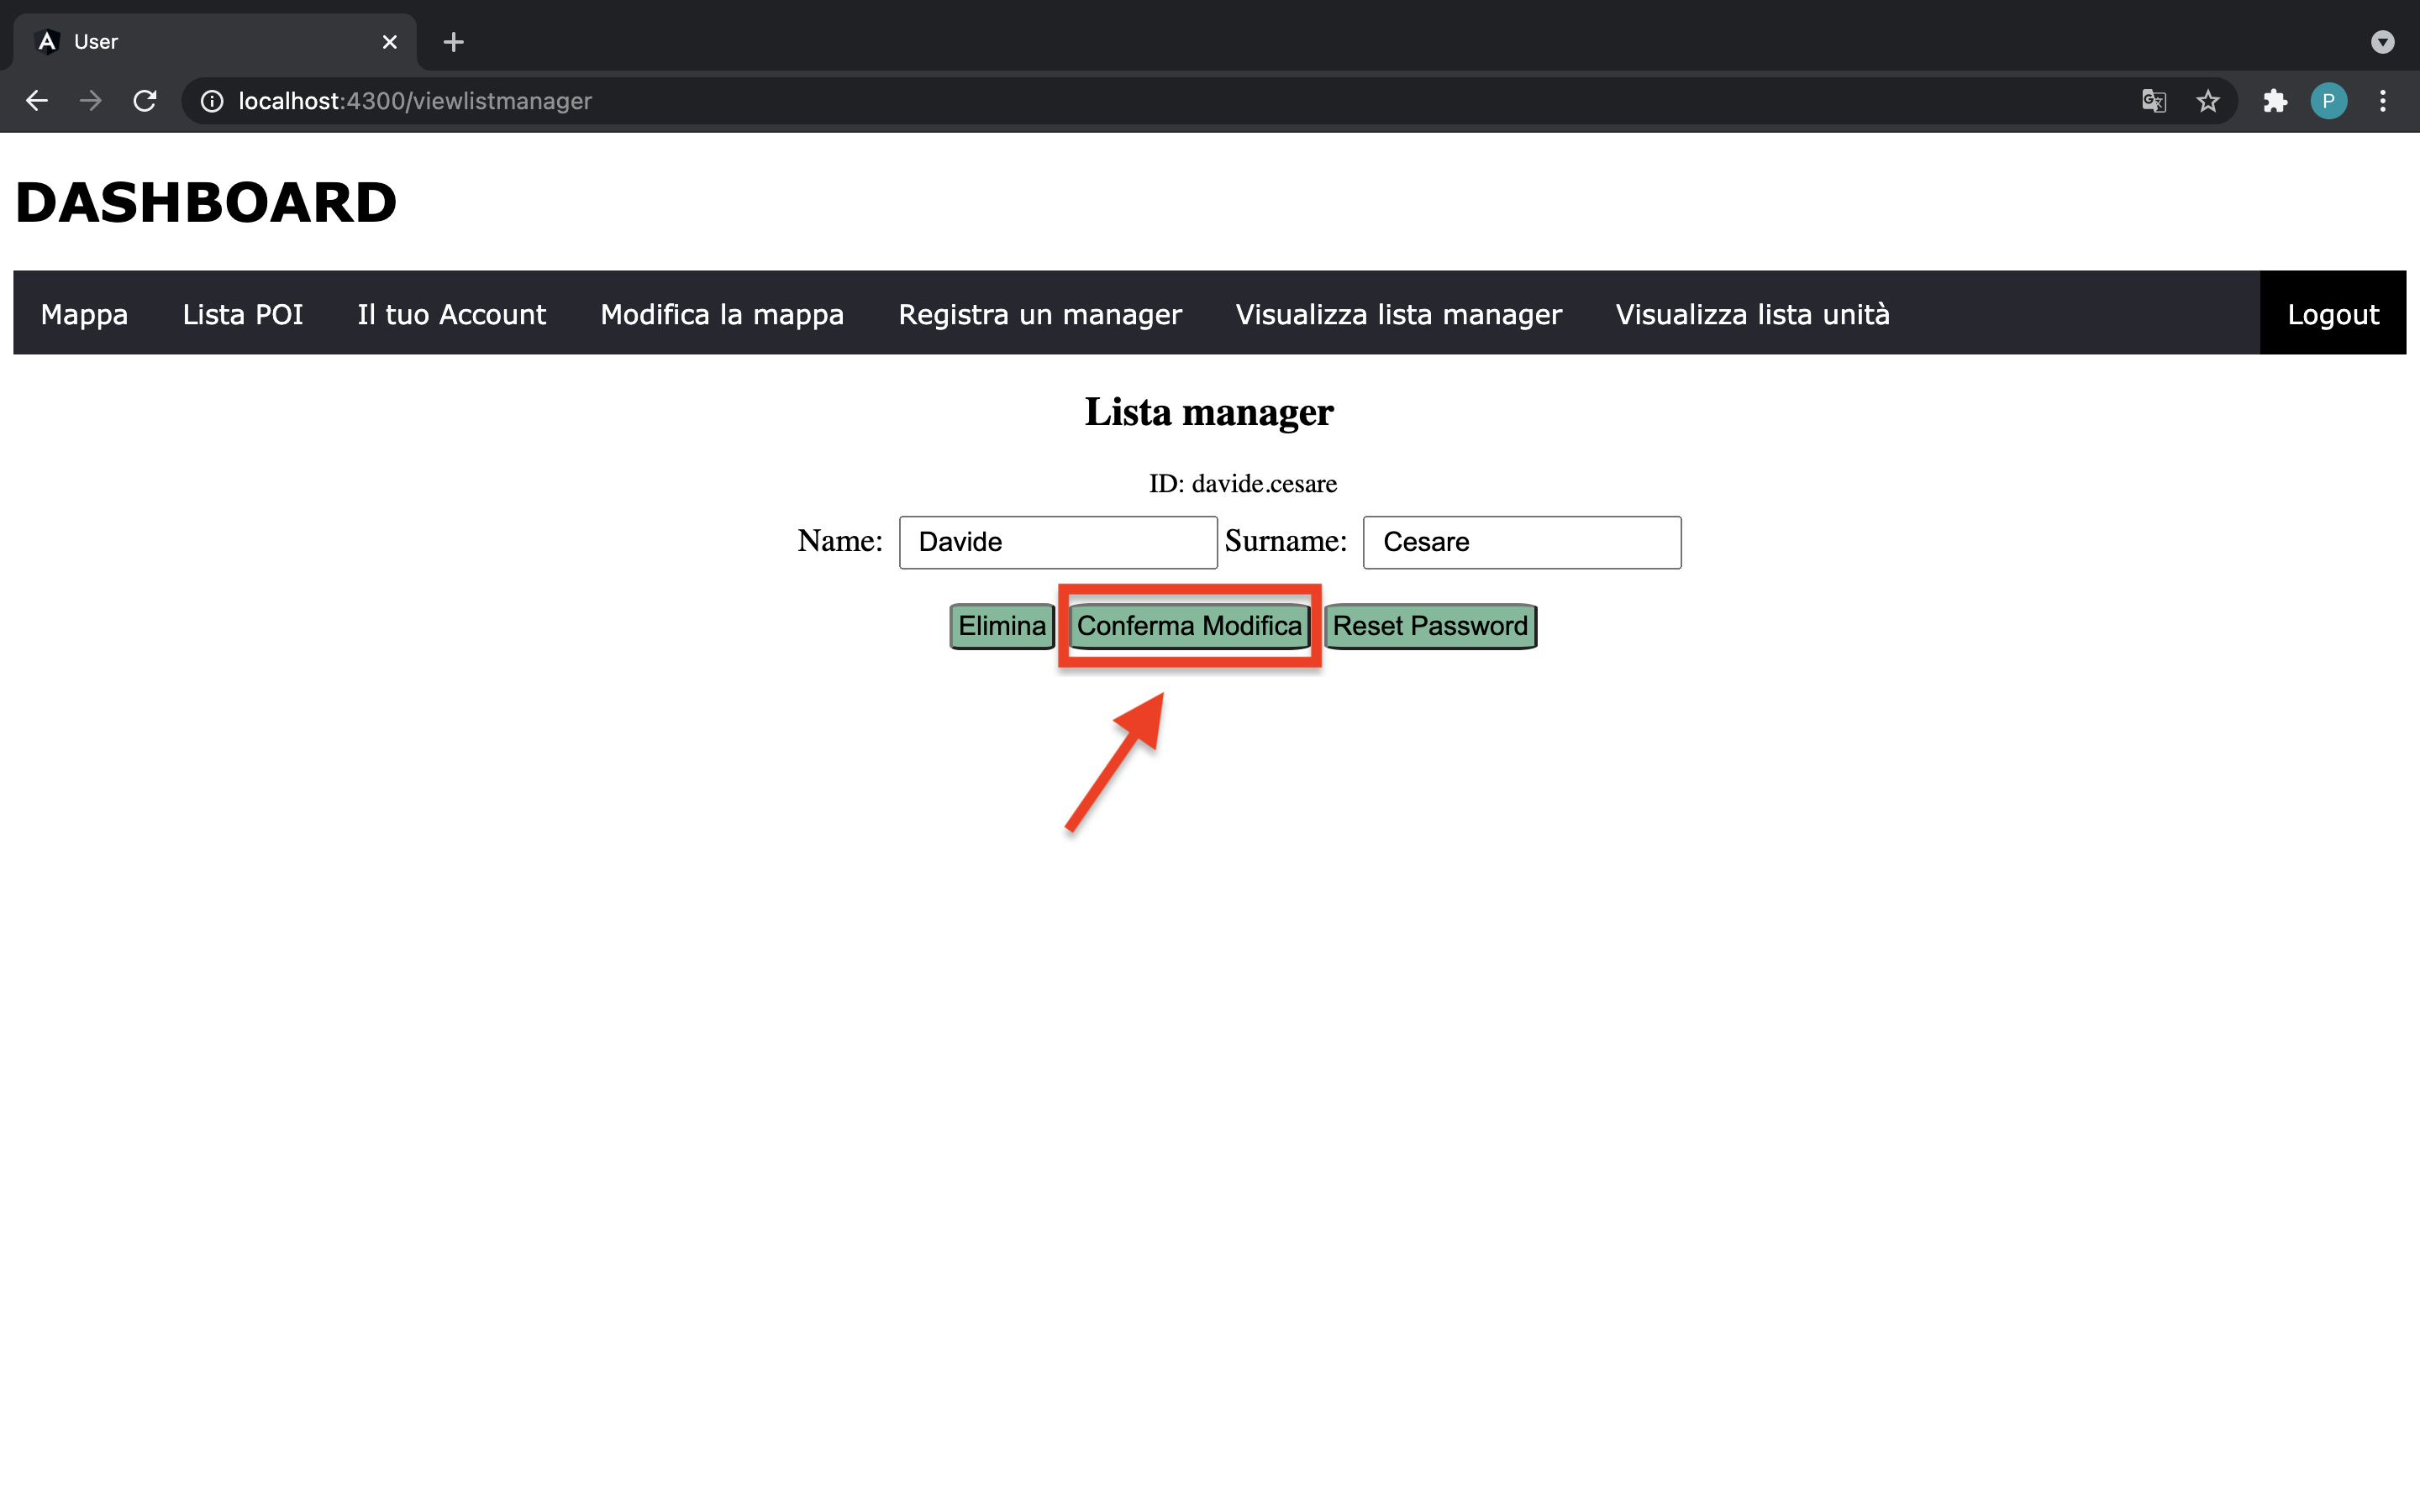
\includegraphics[scale=0.12]{res/images/modificamanager.png}
                \caption{Istantanea dello schermo per la modifica di un utente}
            \end{figure}
            \item premere il pulsate "Elimina" per cancellare definitivamente un account dal sistema;
            \begin{figure}[H]
                \centering
                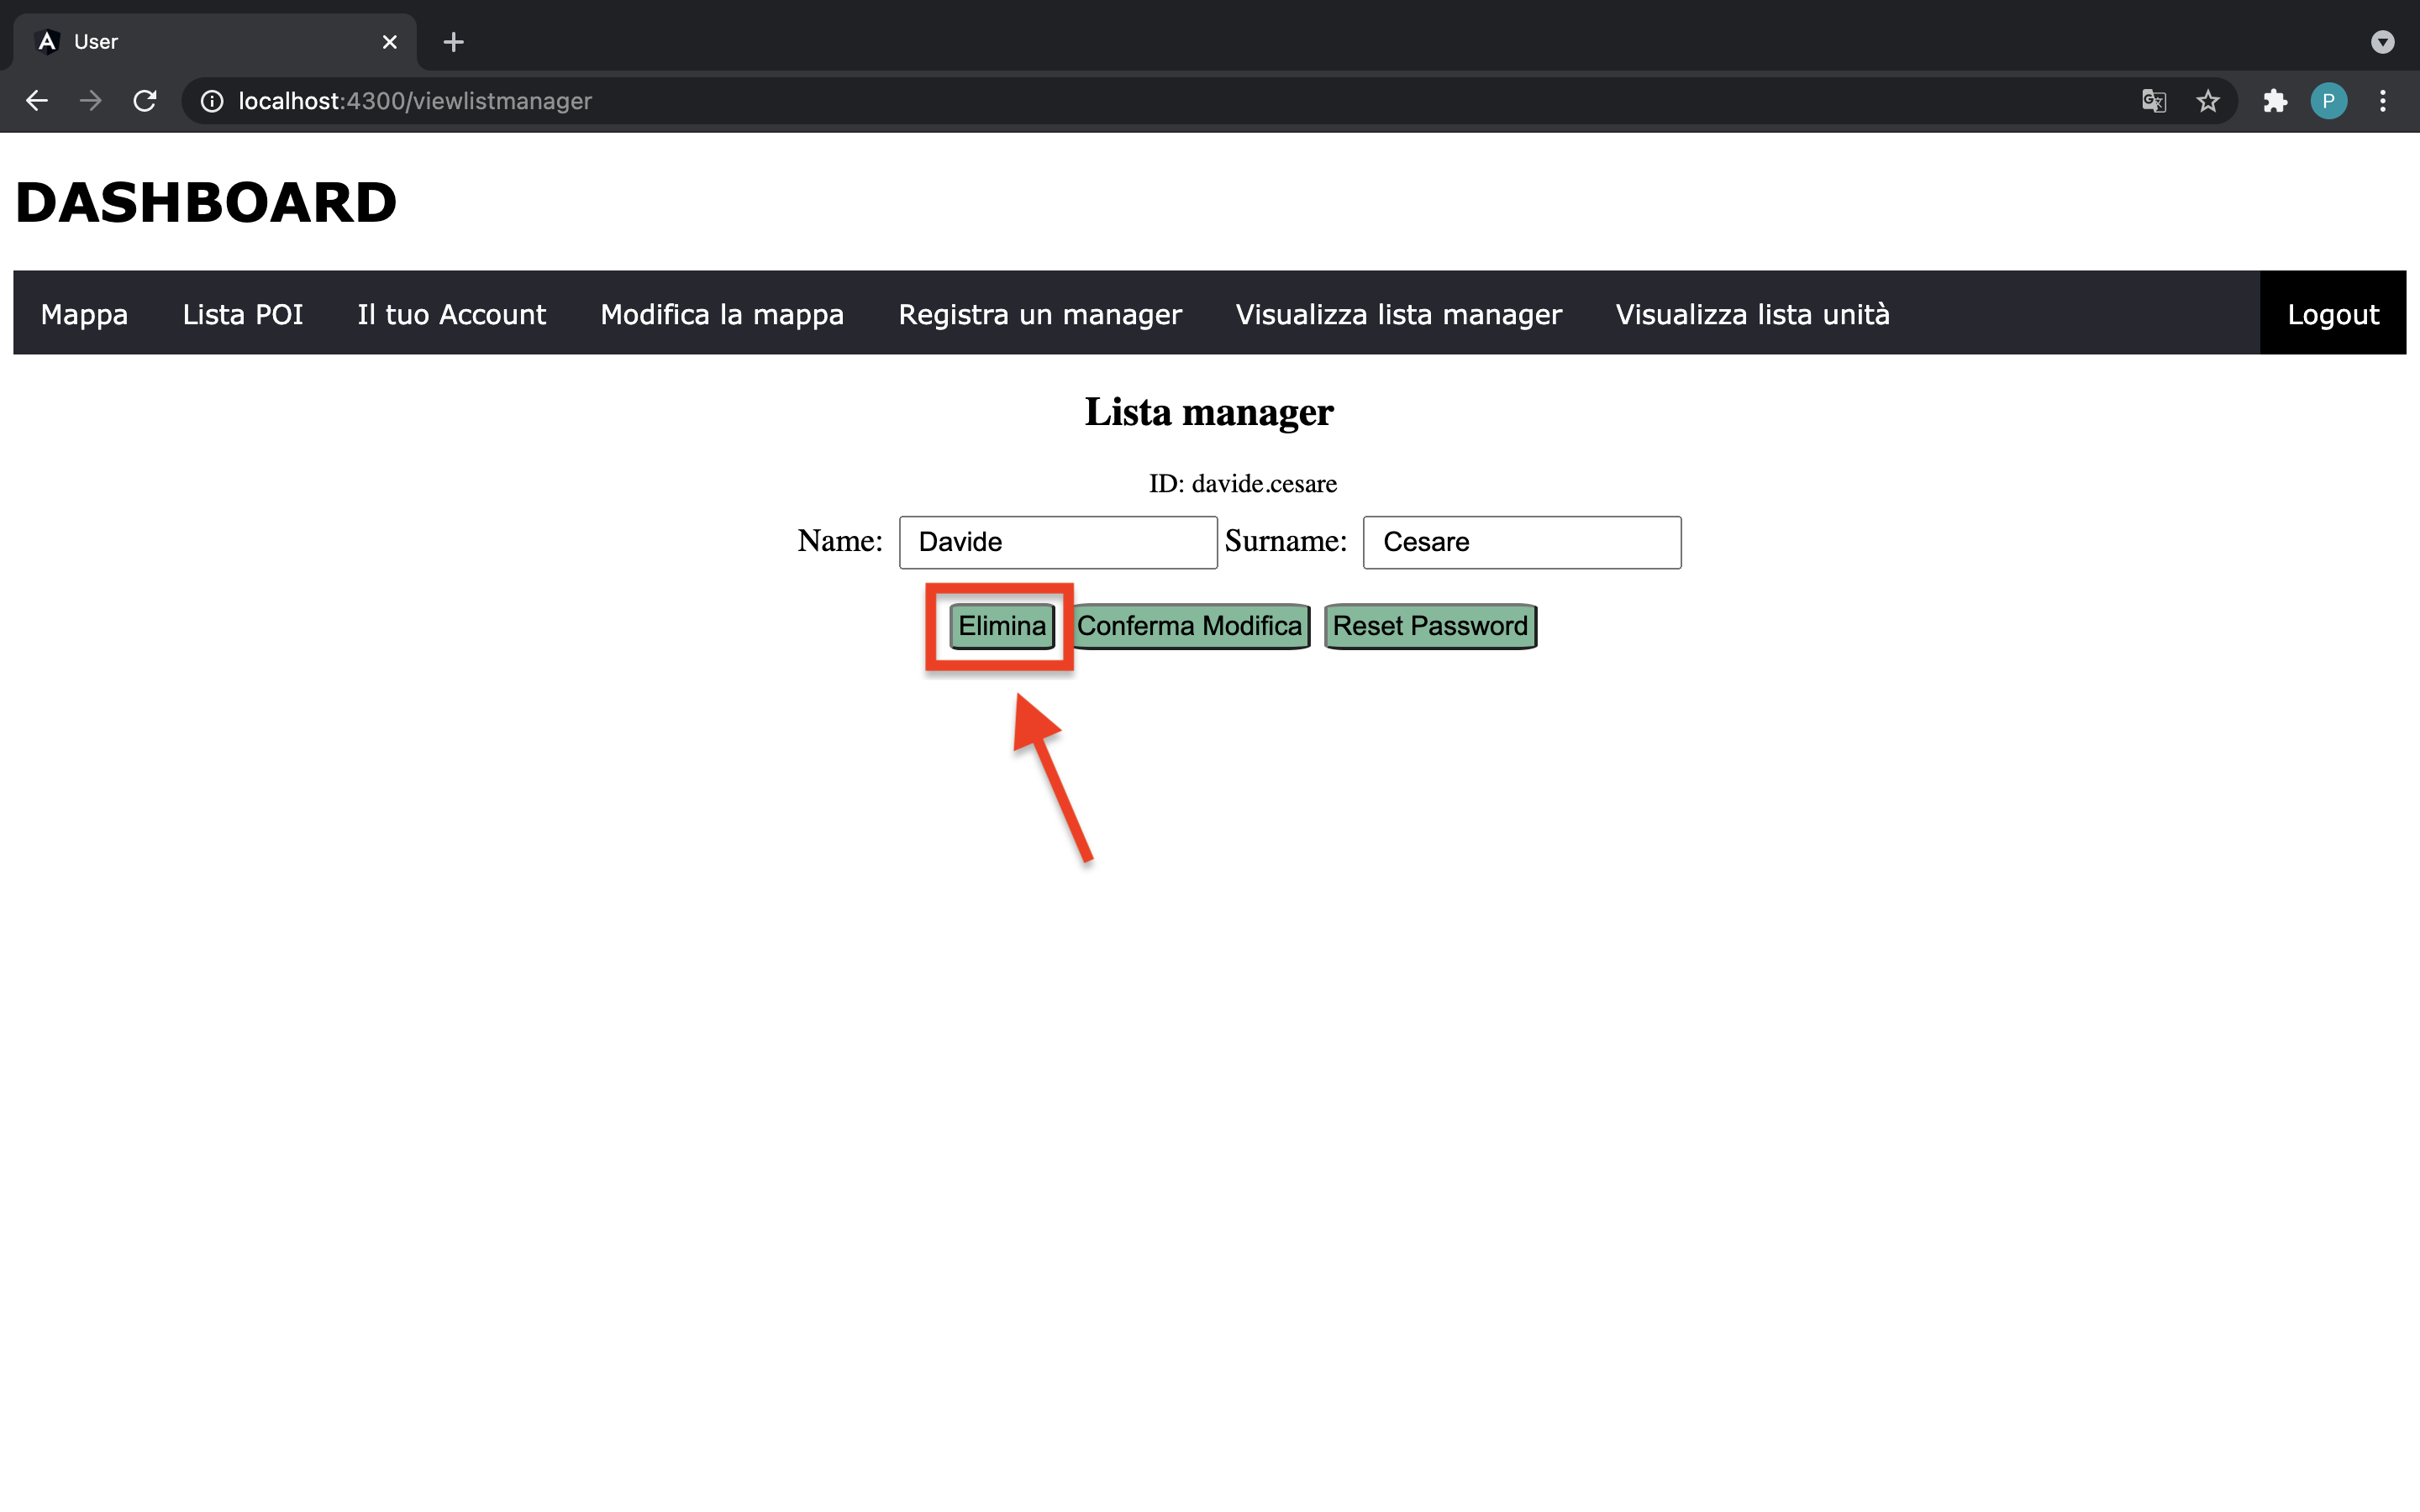
\includegraphics[scale=0.12]{res/images/eliminamanager.png}
                \caption{Istantanea dello schermo per l'eliminazione di un utente}
            \end{figure}
            \item premere il pulsante "Reset Password" per cambiare la password di un utente in caso di smarrimento; 
            \begin{figure}[H]
                \centering
                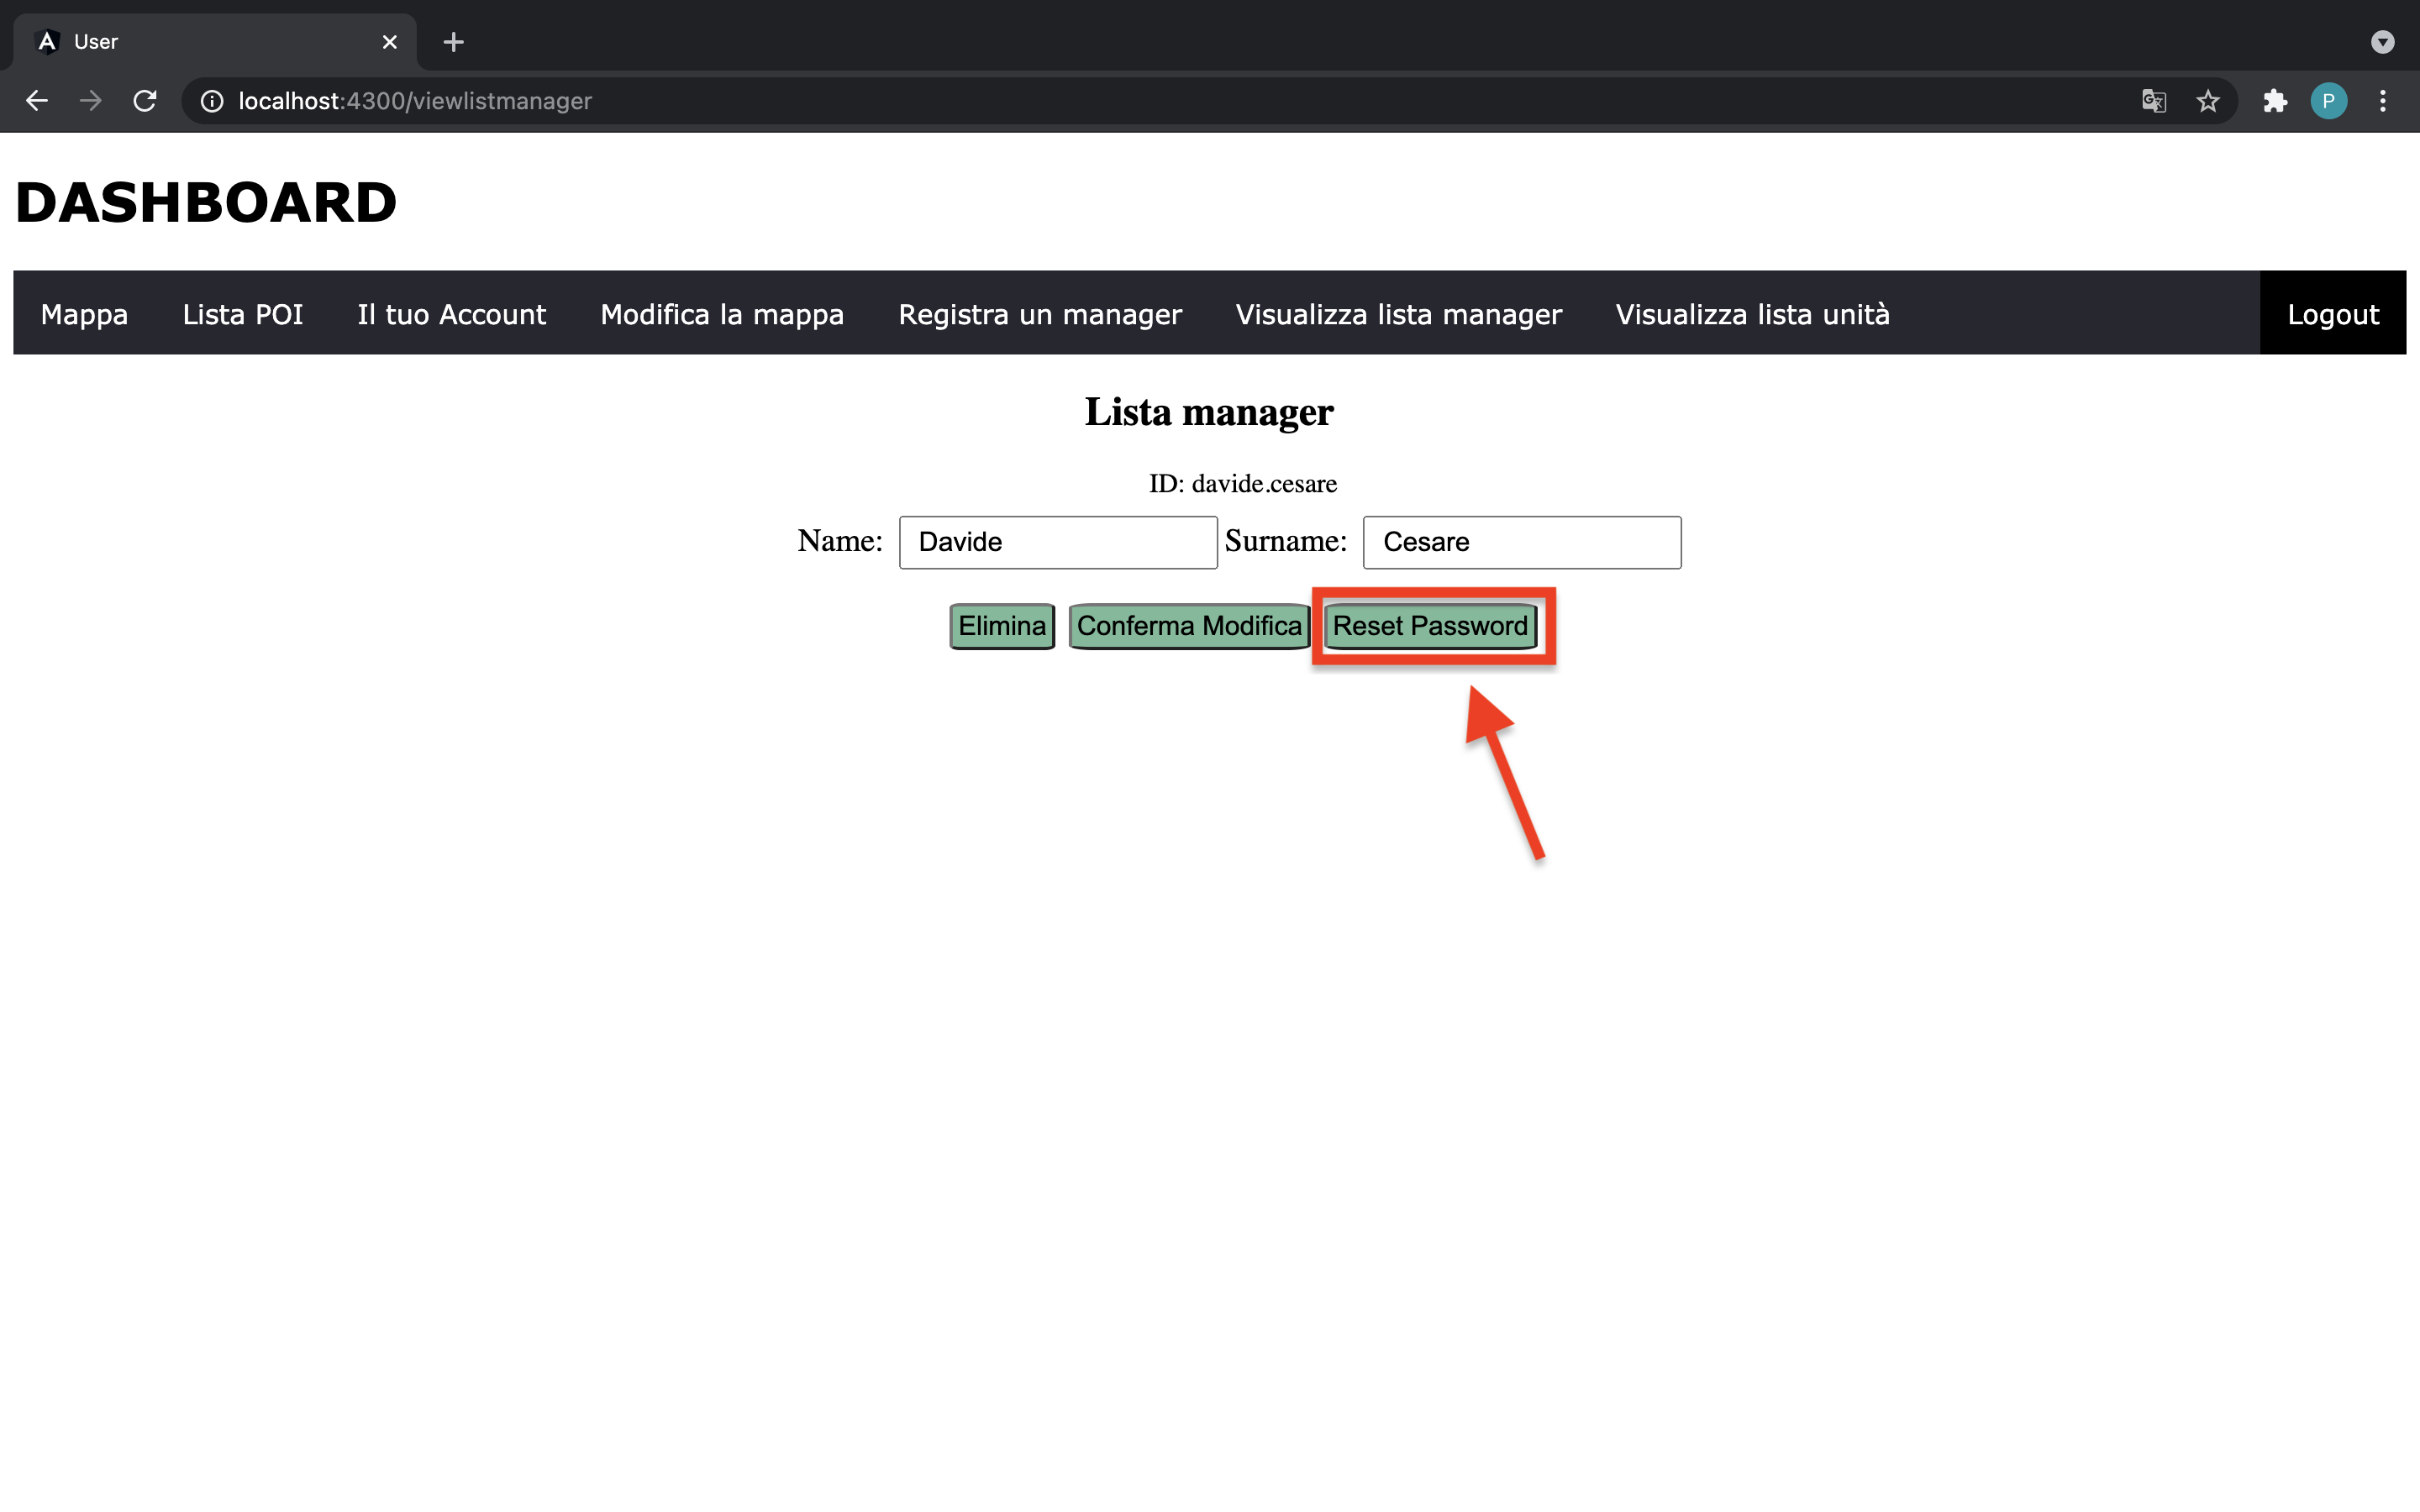
\includegraphics[scale=0.12]{res/images/resetpassword1.png}
                \caption{Istantanea dello schermo per il reset di una password}
            \end{figure}
            \item verrà visualizzata a video la nuova password.
            \begin{figure}[H]
                \centering
                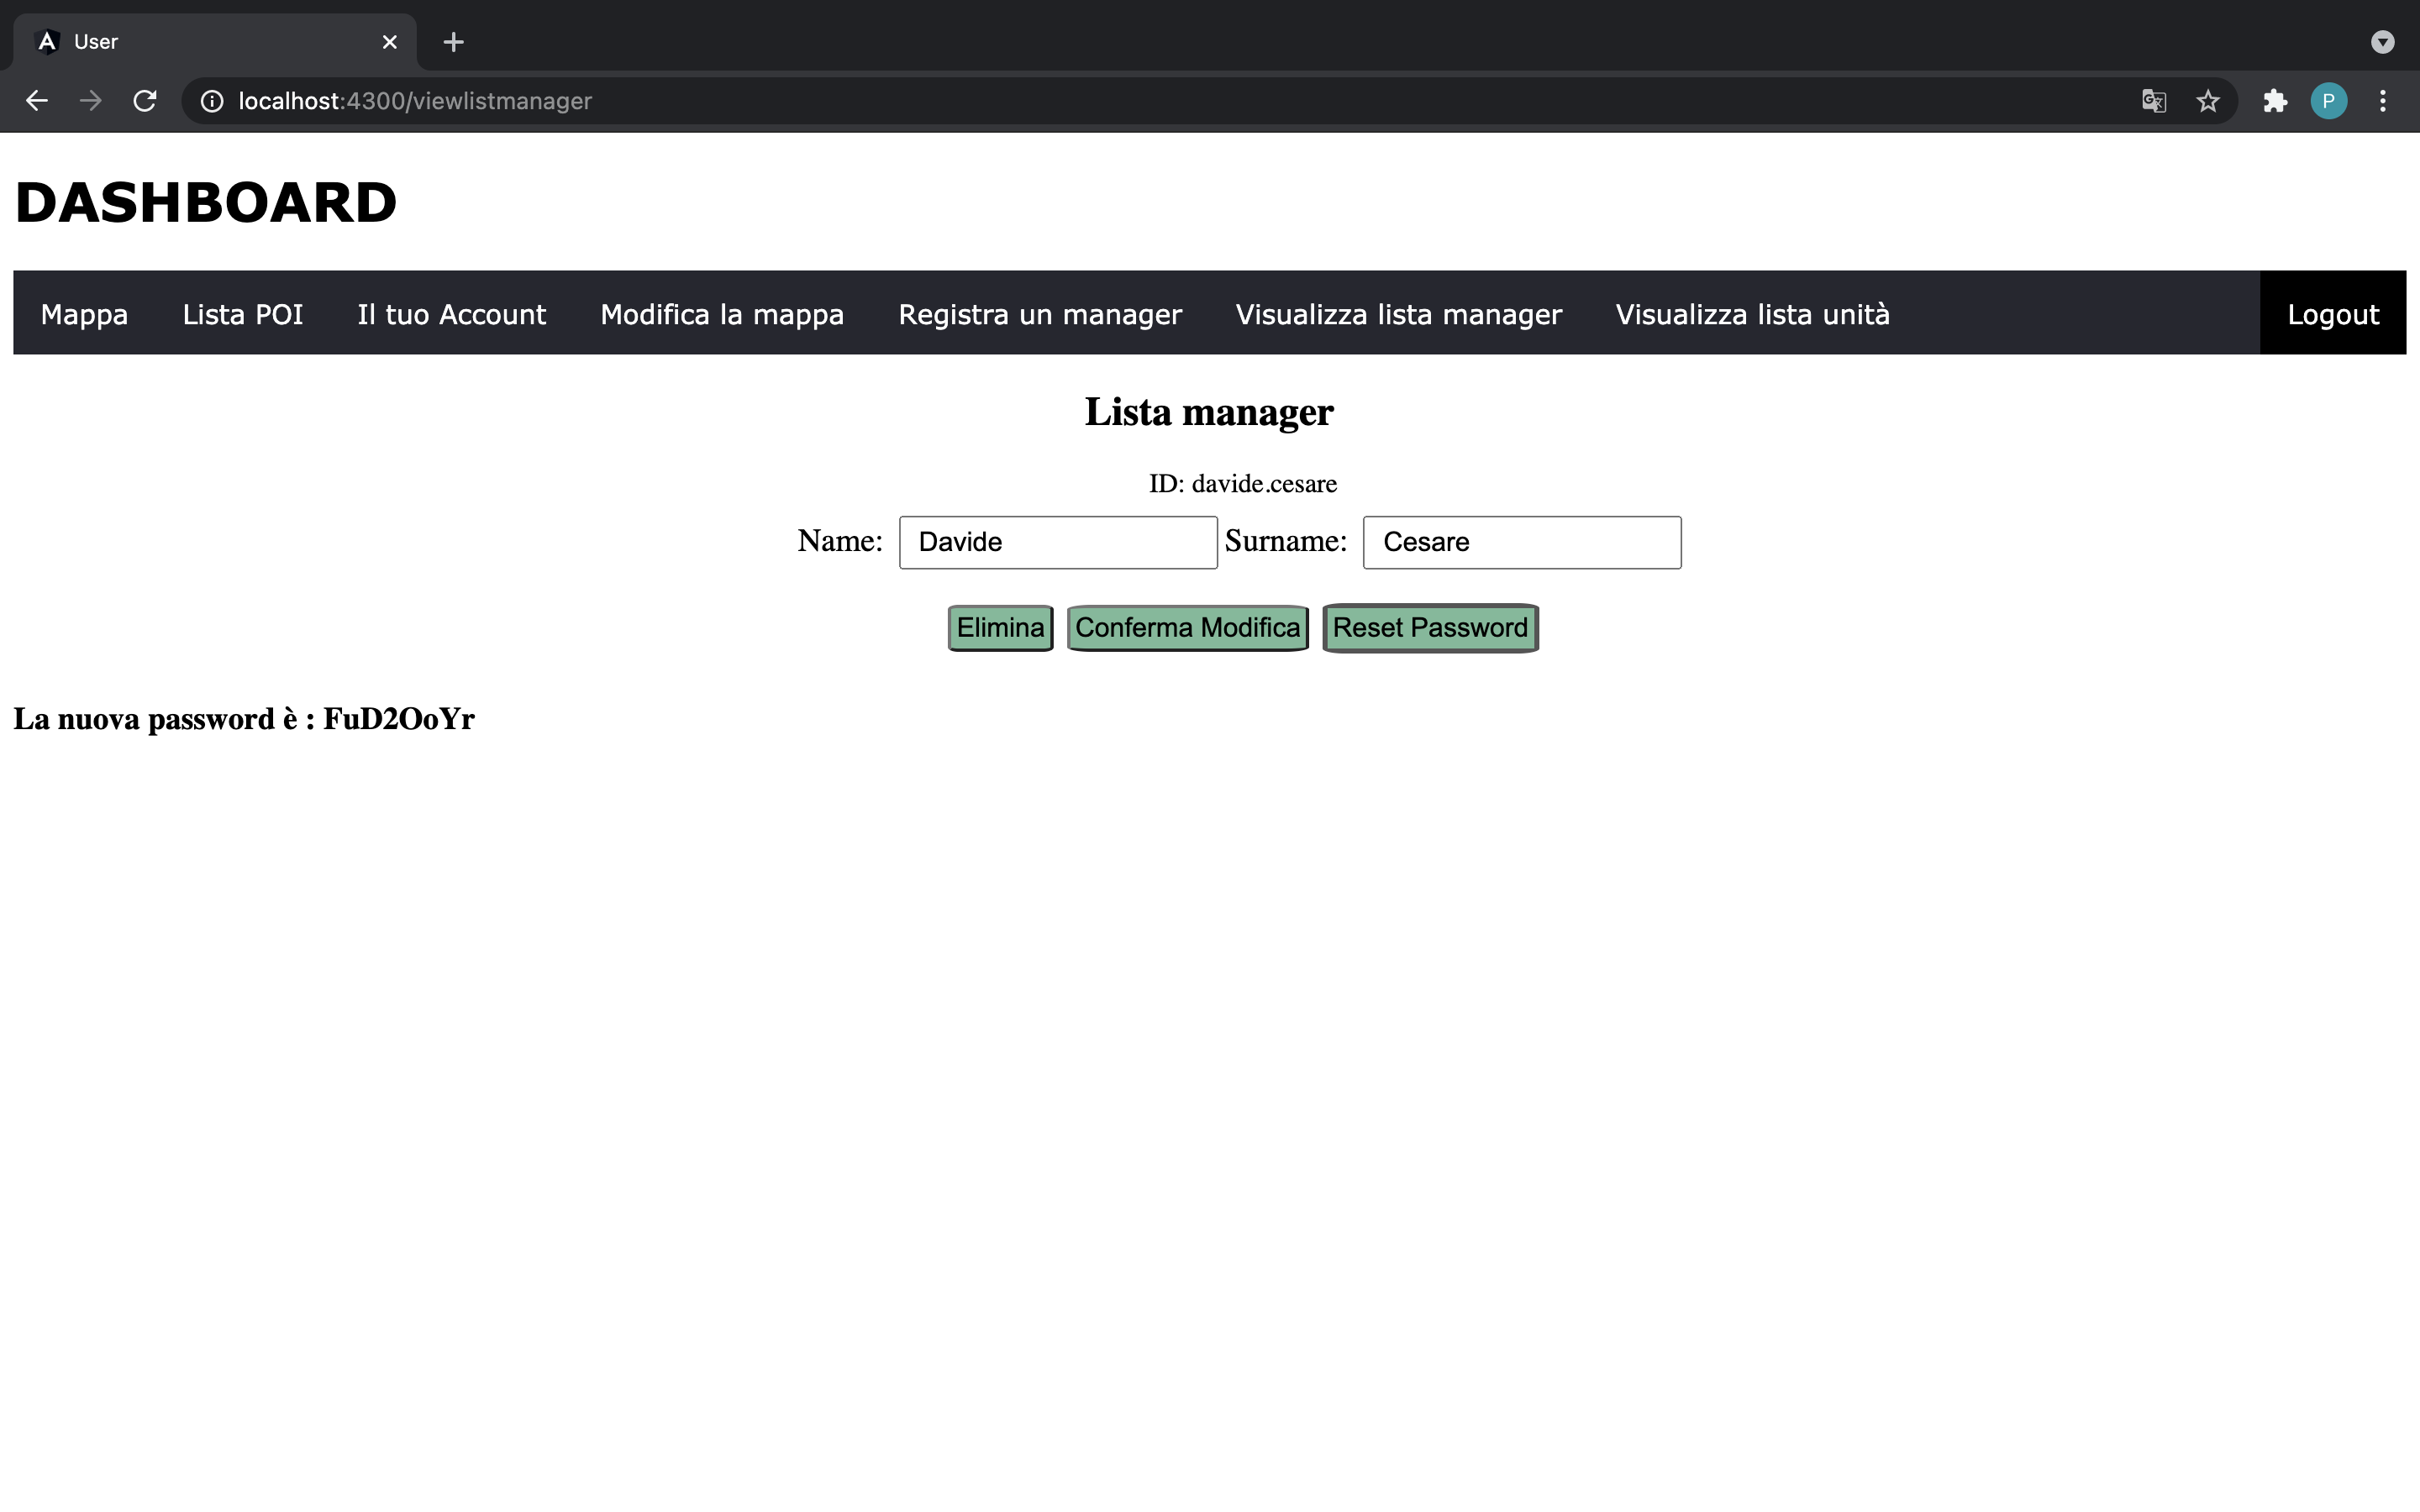
\includegraphics[scale=0.12]{res/images/resetpassowrd2.png}
                \caption{Istantanea dello schermo per il reset di una password}
            \end{figure}
        \end{itemize}
\end{itemize}


\subsection{Modifica mappa del magazzino}
\begin{itemize}
    \item Dopo l'autenticazione, tramite il menù selezionare il pulsante "Modifica la mappa";
    \begin{figure}[H]
        \centering
        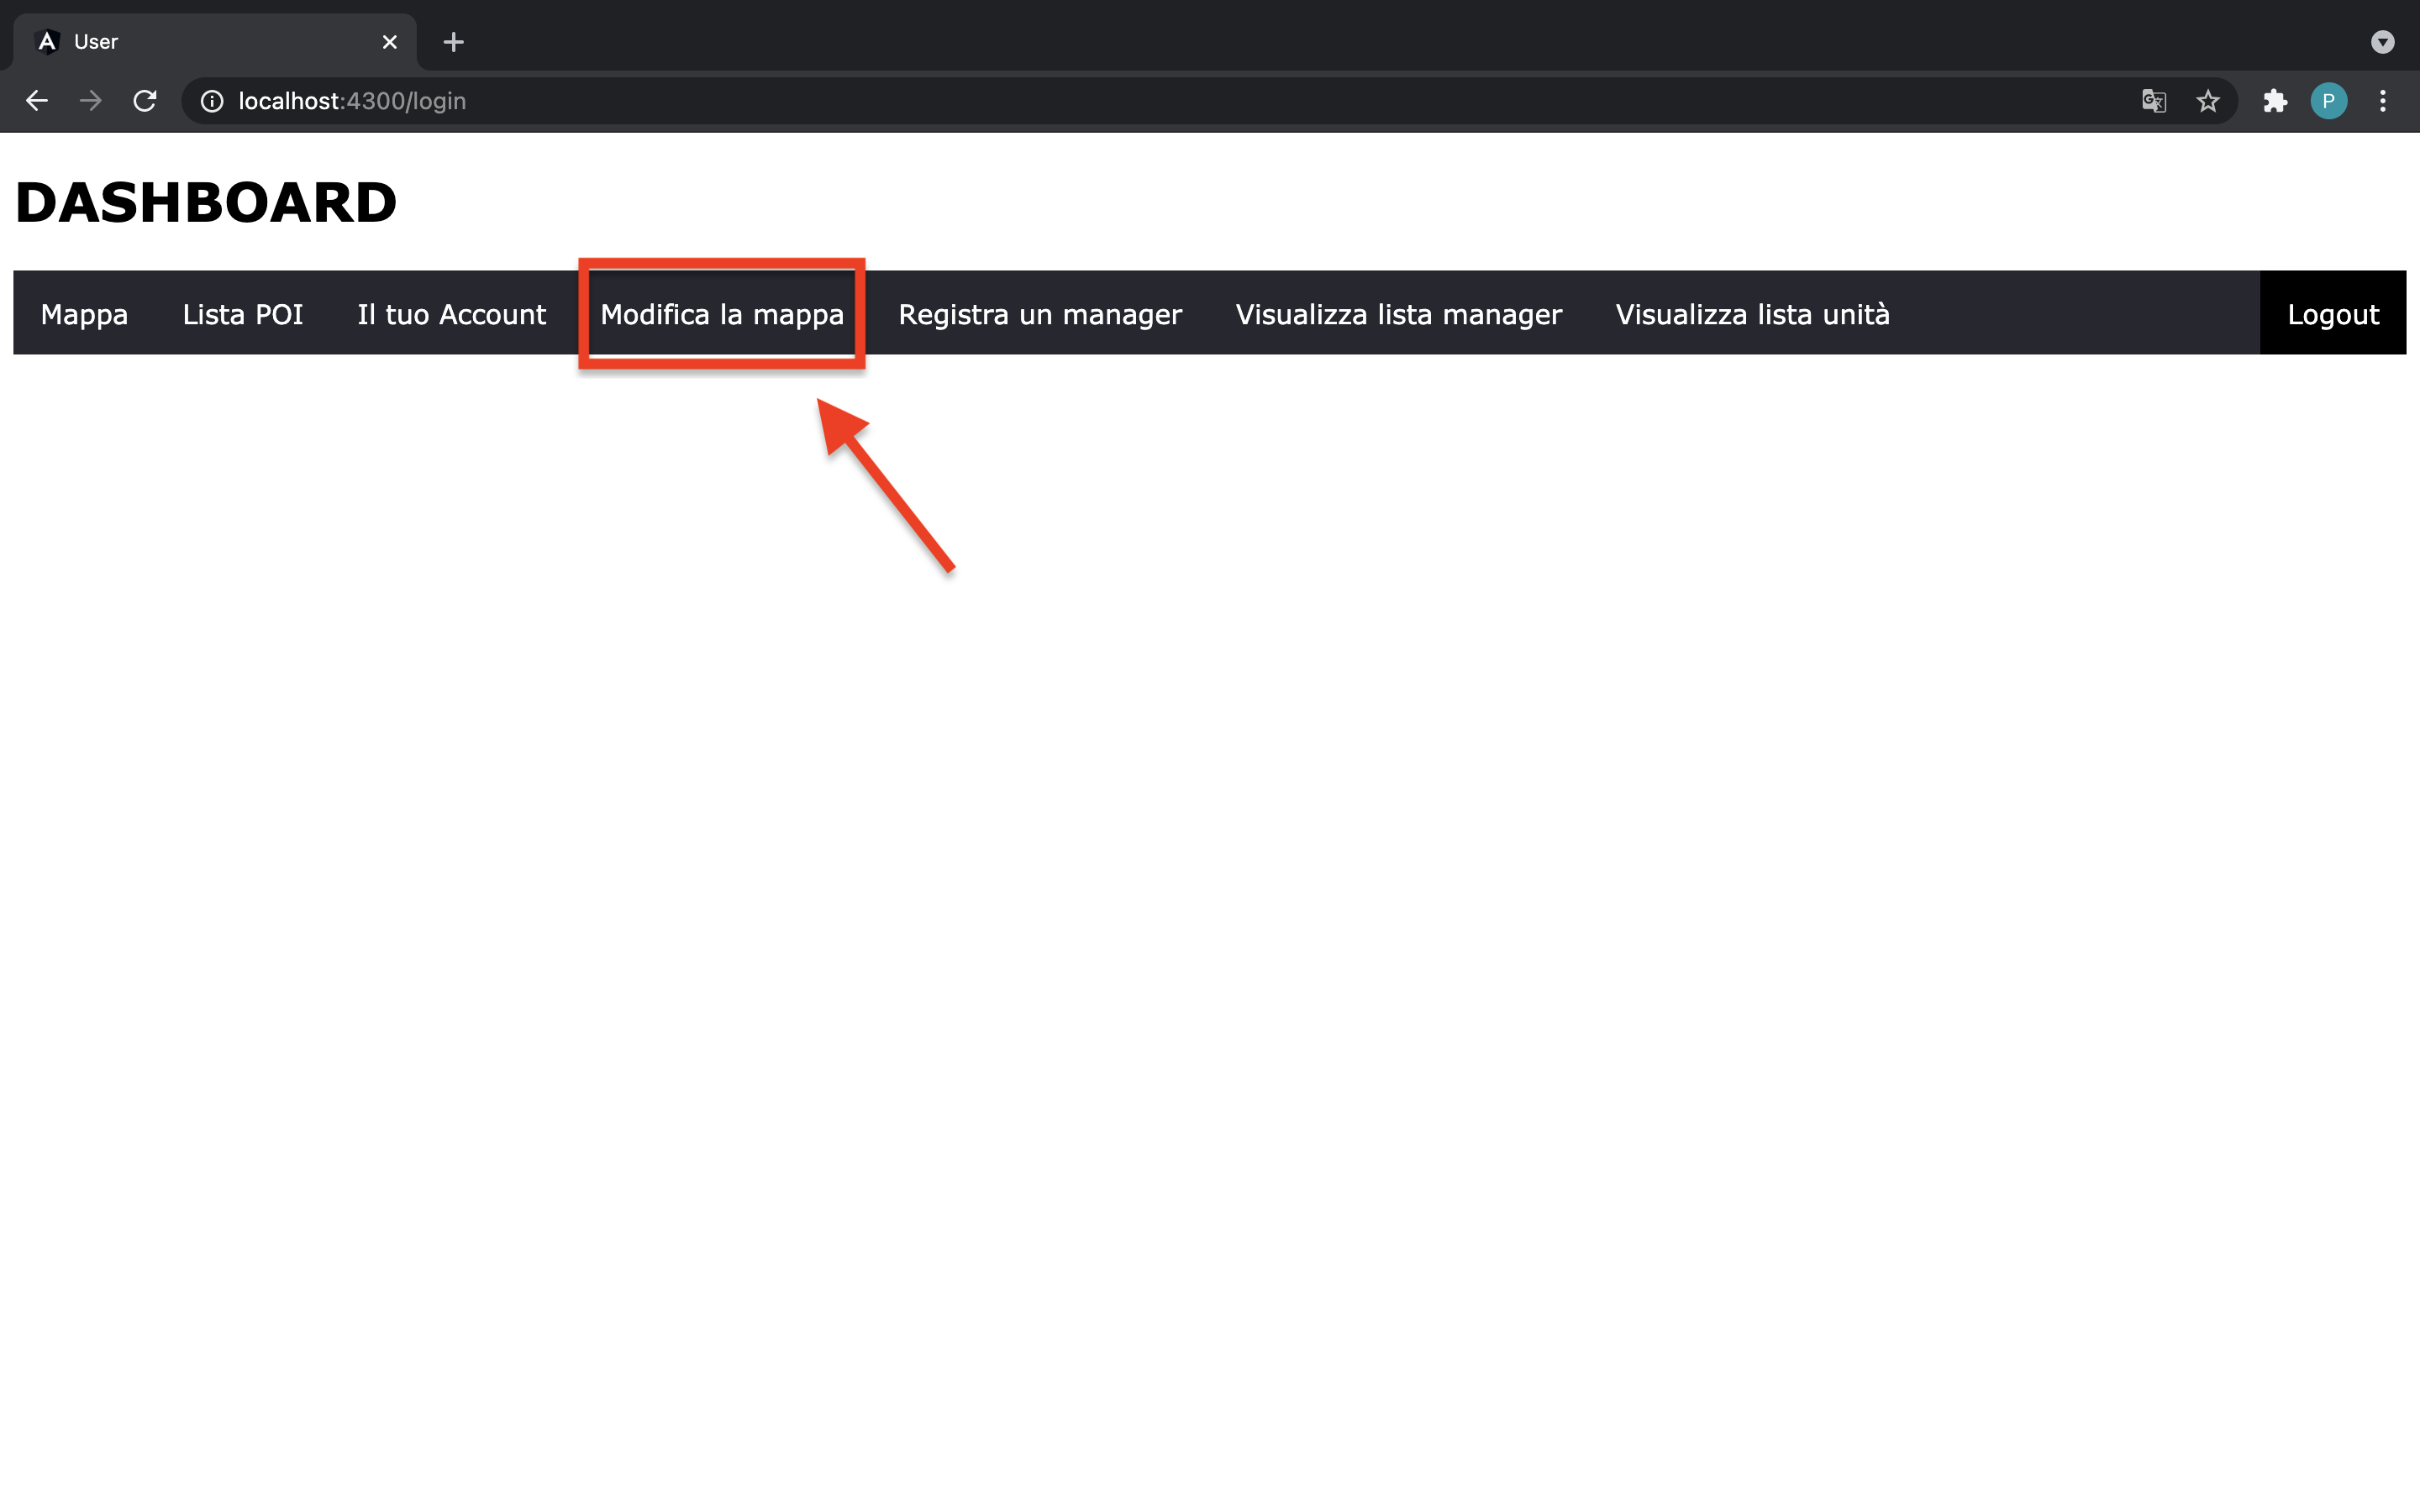
\includegraphics[scale=0.12]{res/images/dashboard6.png}
        \caption{Istantanea dello schermo con indicazione per la modifica della mappa}
    \end{figure}
    \item si viene indirizzati alla pagina con la rappresentazione della mappa;
    \item è possibile intraprendere le seguenti operazioni:
        \begin{itemize}
            \item aggiungere una riga: \\premere sul pulsante "Aggiungi riga" per ampliare la planimetria di una riga;
            \begin{figure}[H]
                \centering
                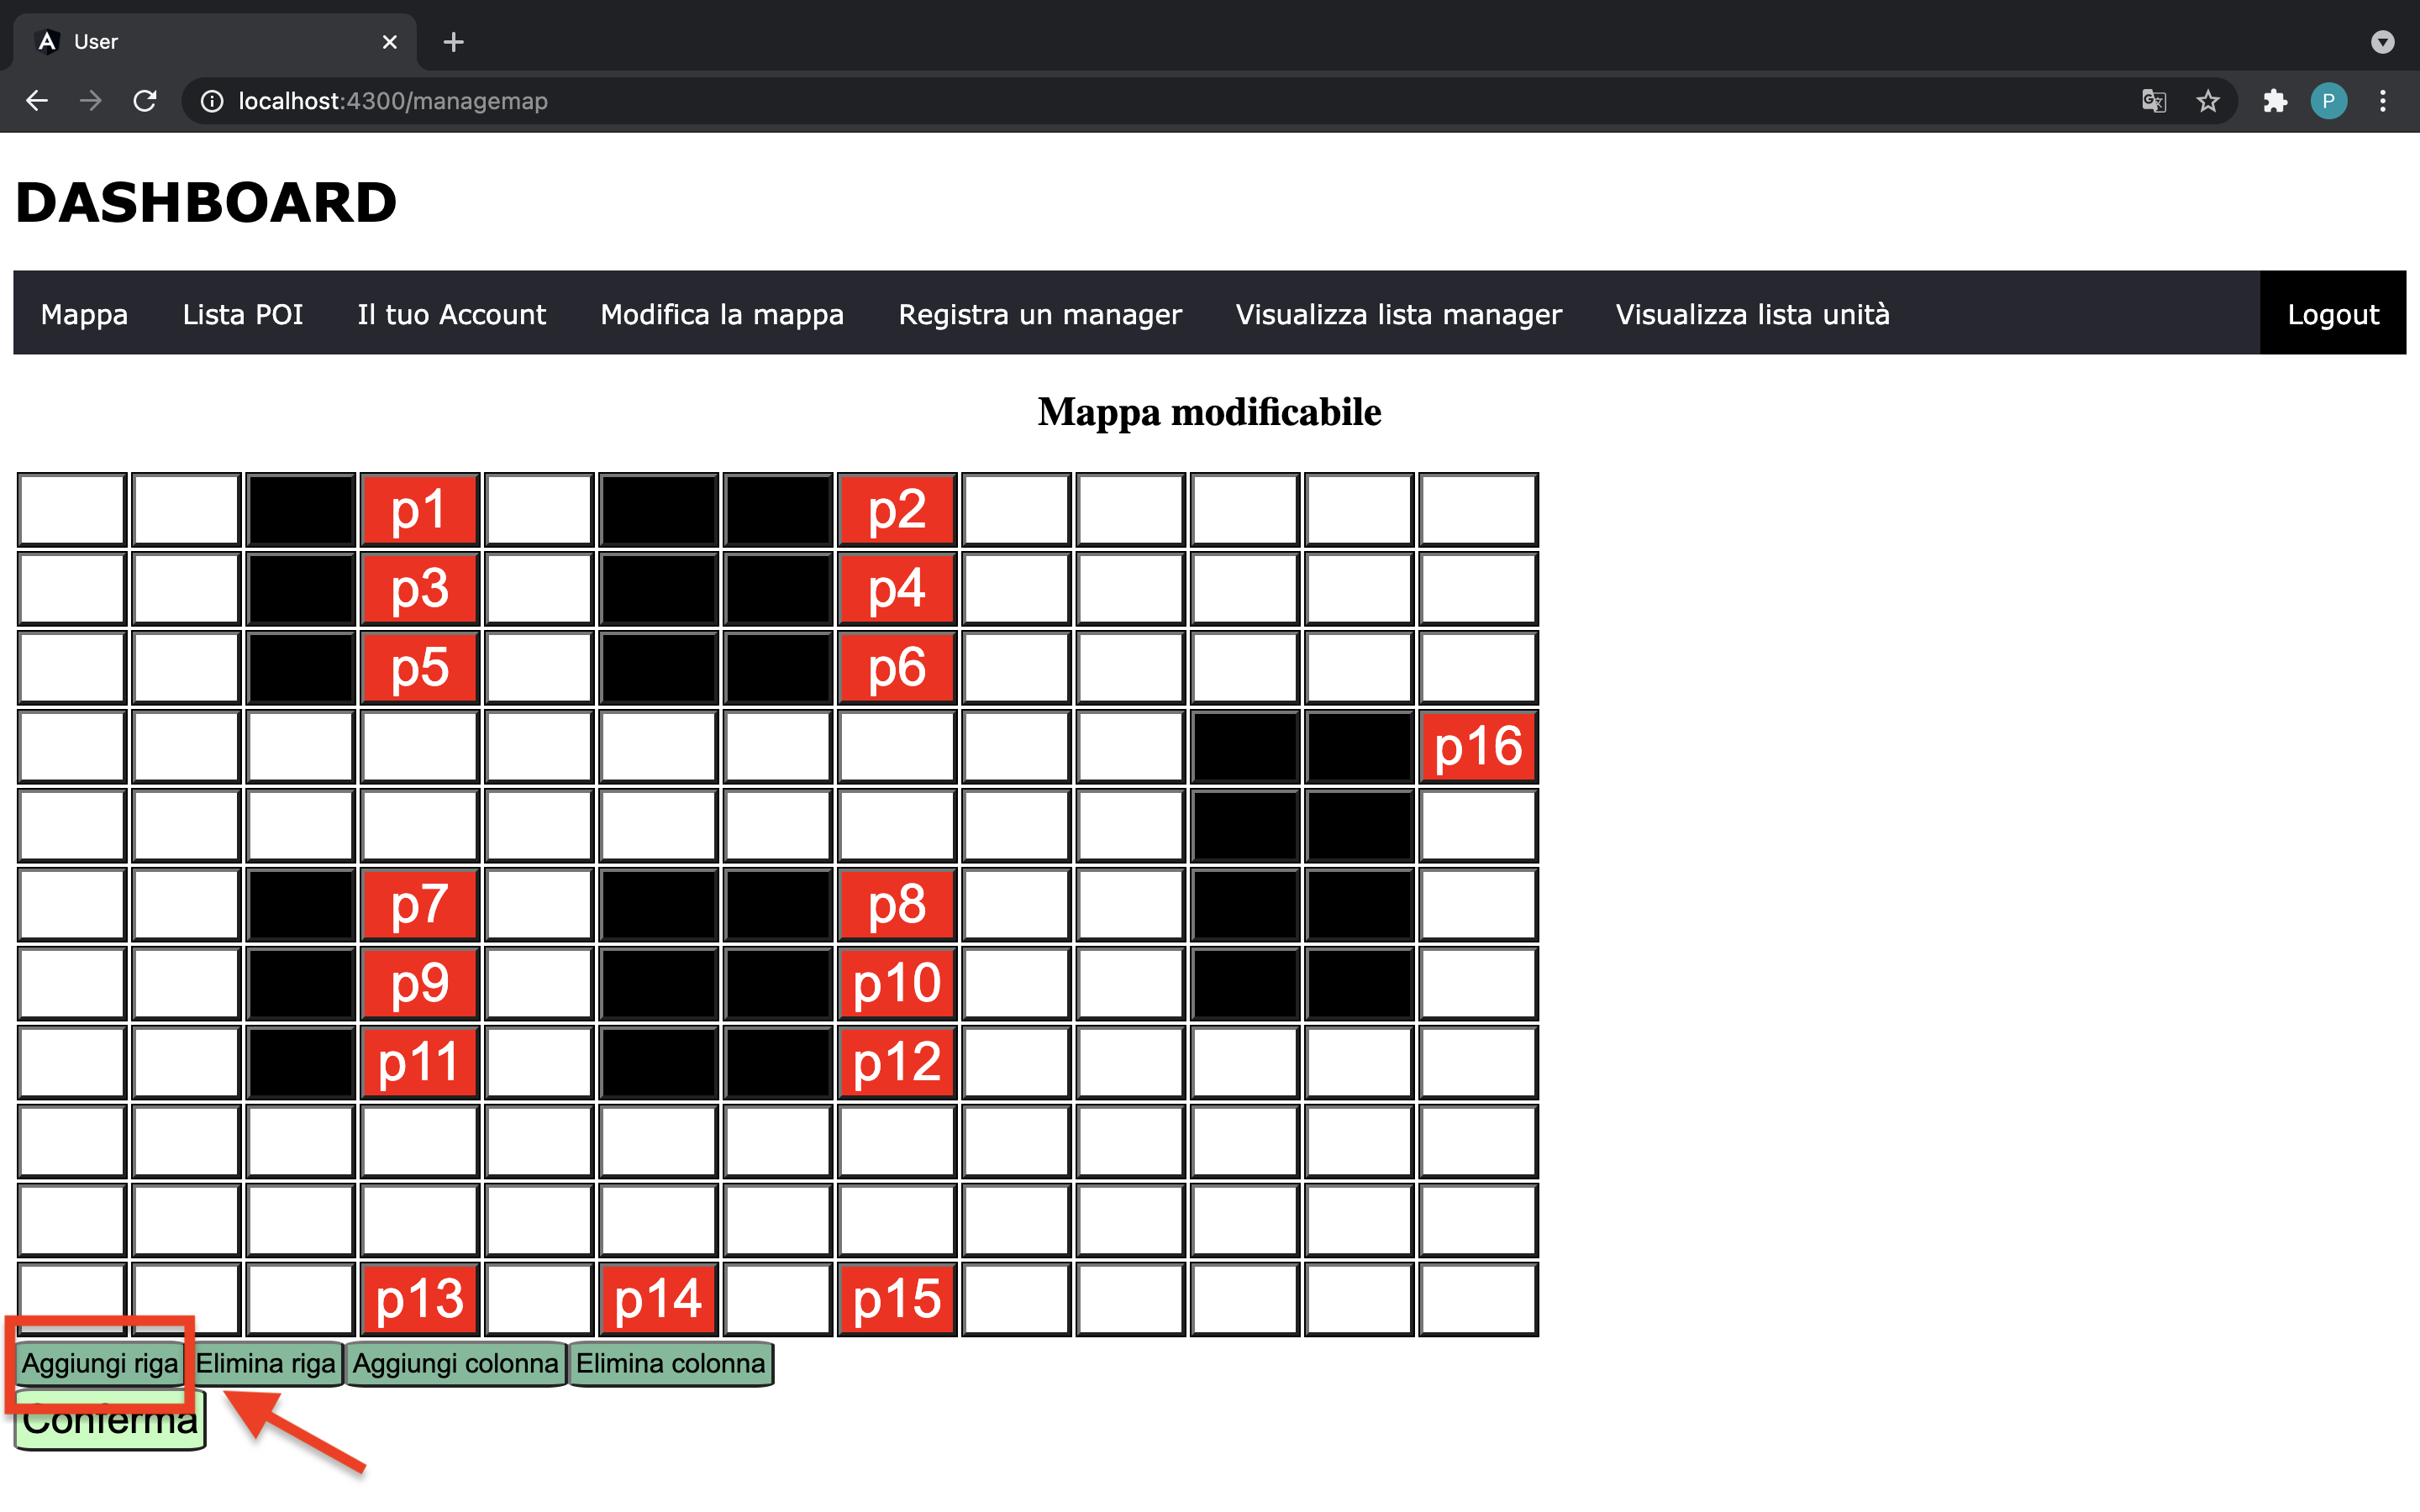
\includegraphics[scale=0.12]{res/images/modificamappa1.png}
                \caption{Istantanea dello schermo ampliamento mappa per riga}
            \end{figure}
            \item eliminare una riga: \\premere sul pulsante "Elimina riga" per diminuire la planimetria di una riga. Eliminare i POI presenti nell'ultima riga prima di premere il pulsante altrimenti verrà visualizzato un errore e la cancellazione non verrà eseguita;
            \begin{figure}[H]
                \centering
                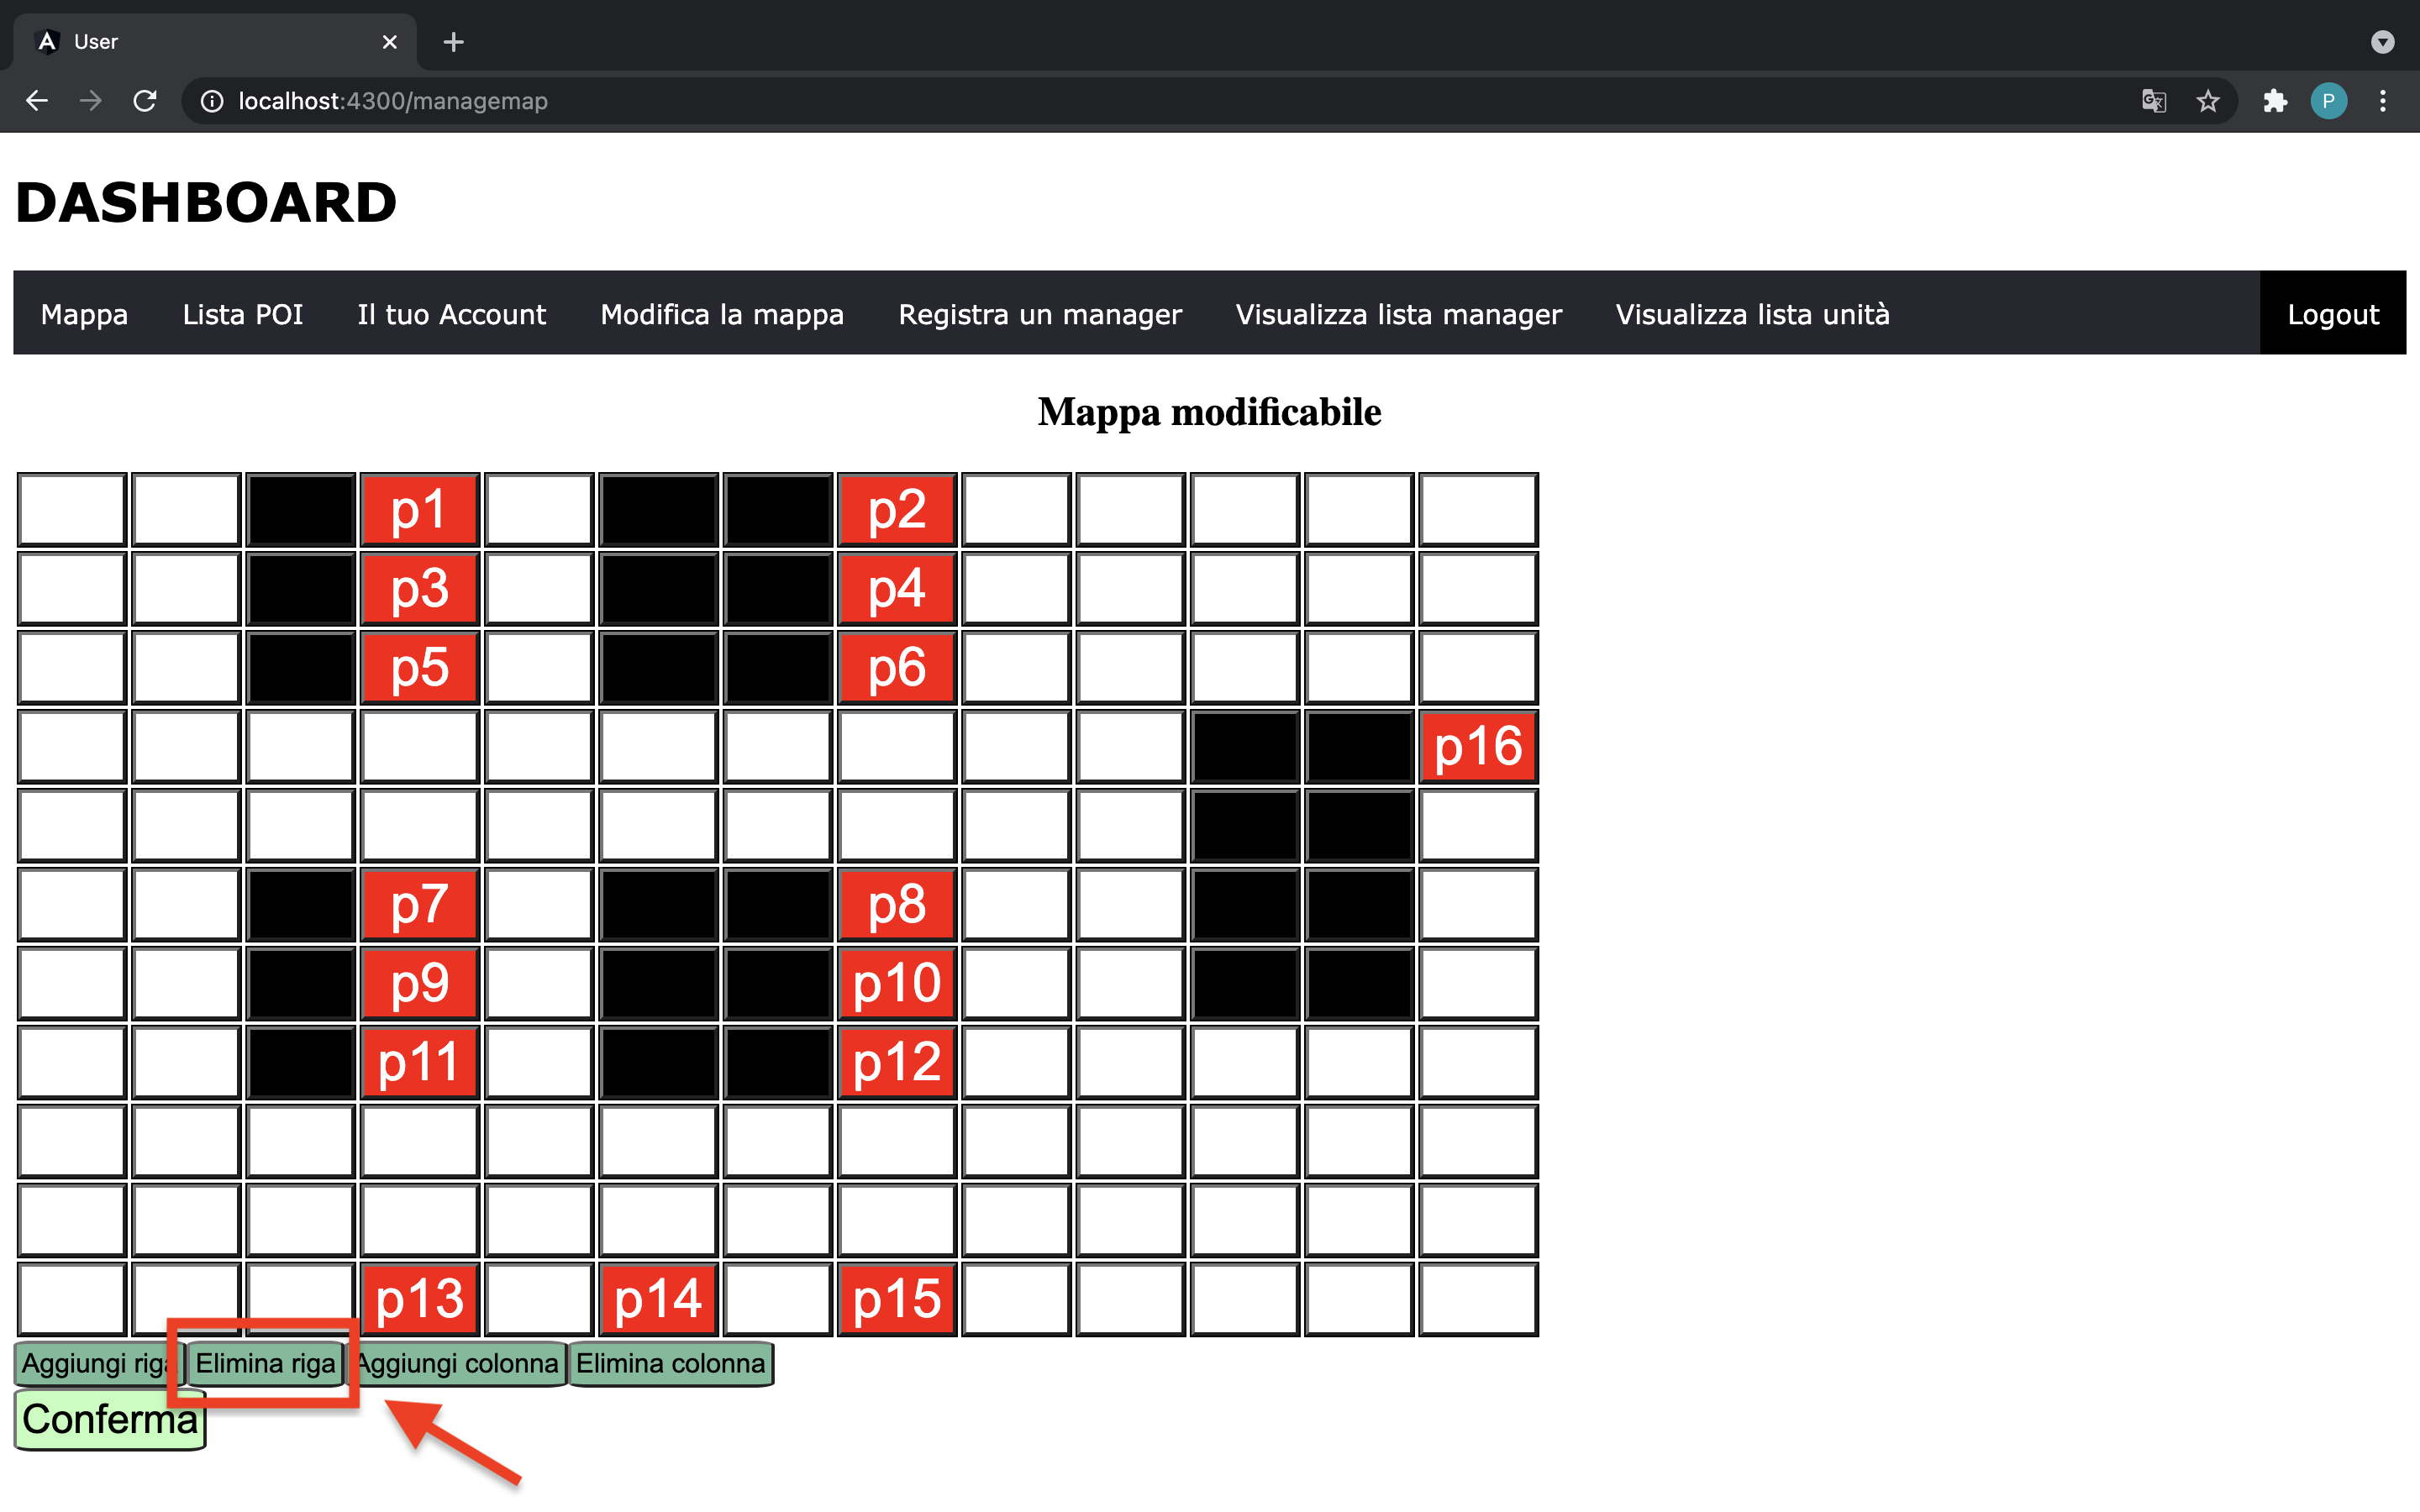
\includegraphics[scale=0.12]{res/images/modificamappa2.png}
                \caption{Istantanea dello schermo diminuzione mappa per riga}
            \end{figure}
            \item aggiungere una colonna: \\premere sul pulsante "Aggiungi colonna" per ampliare la planimetria di una colonna;
            \begin{figure}[H]
                \centering
                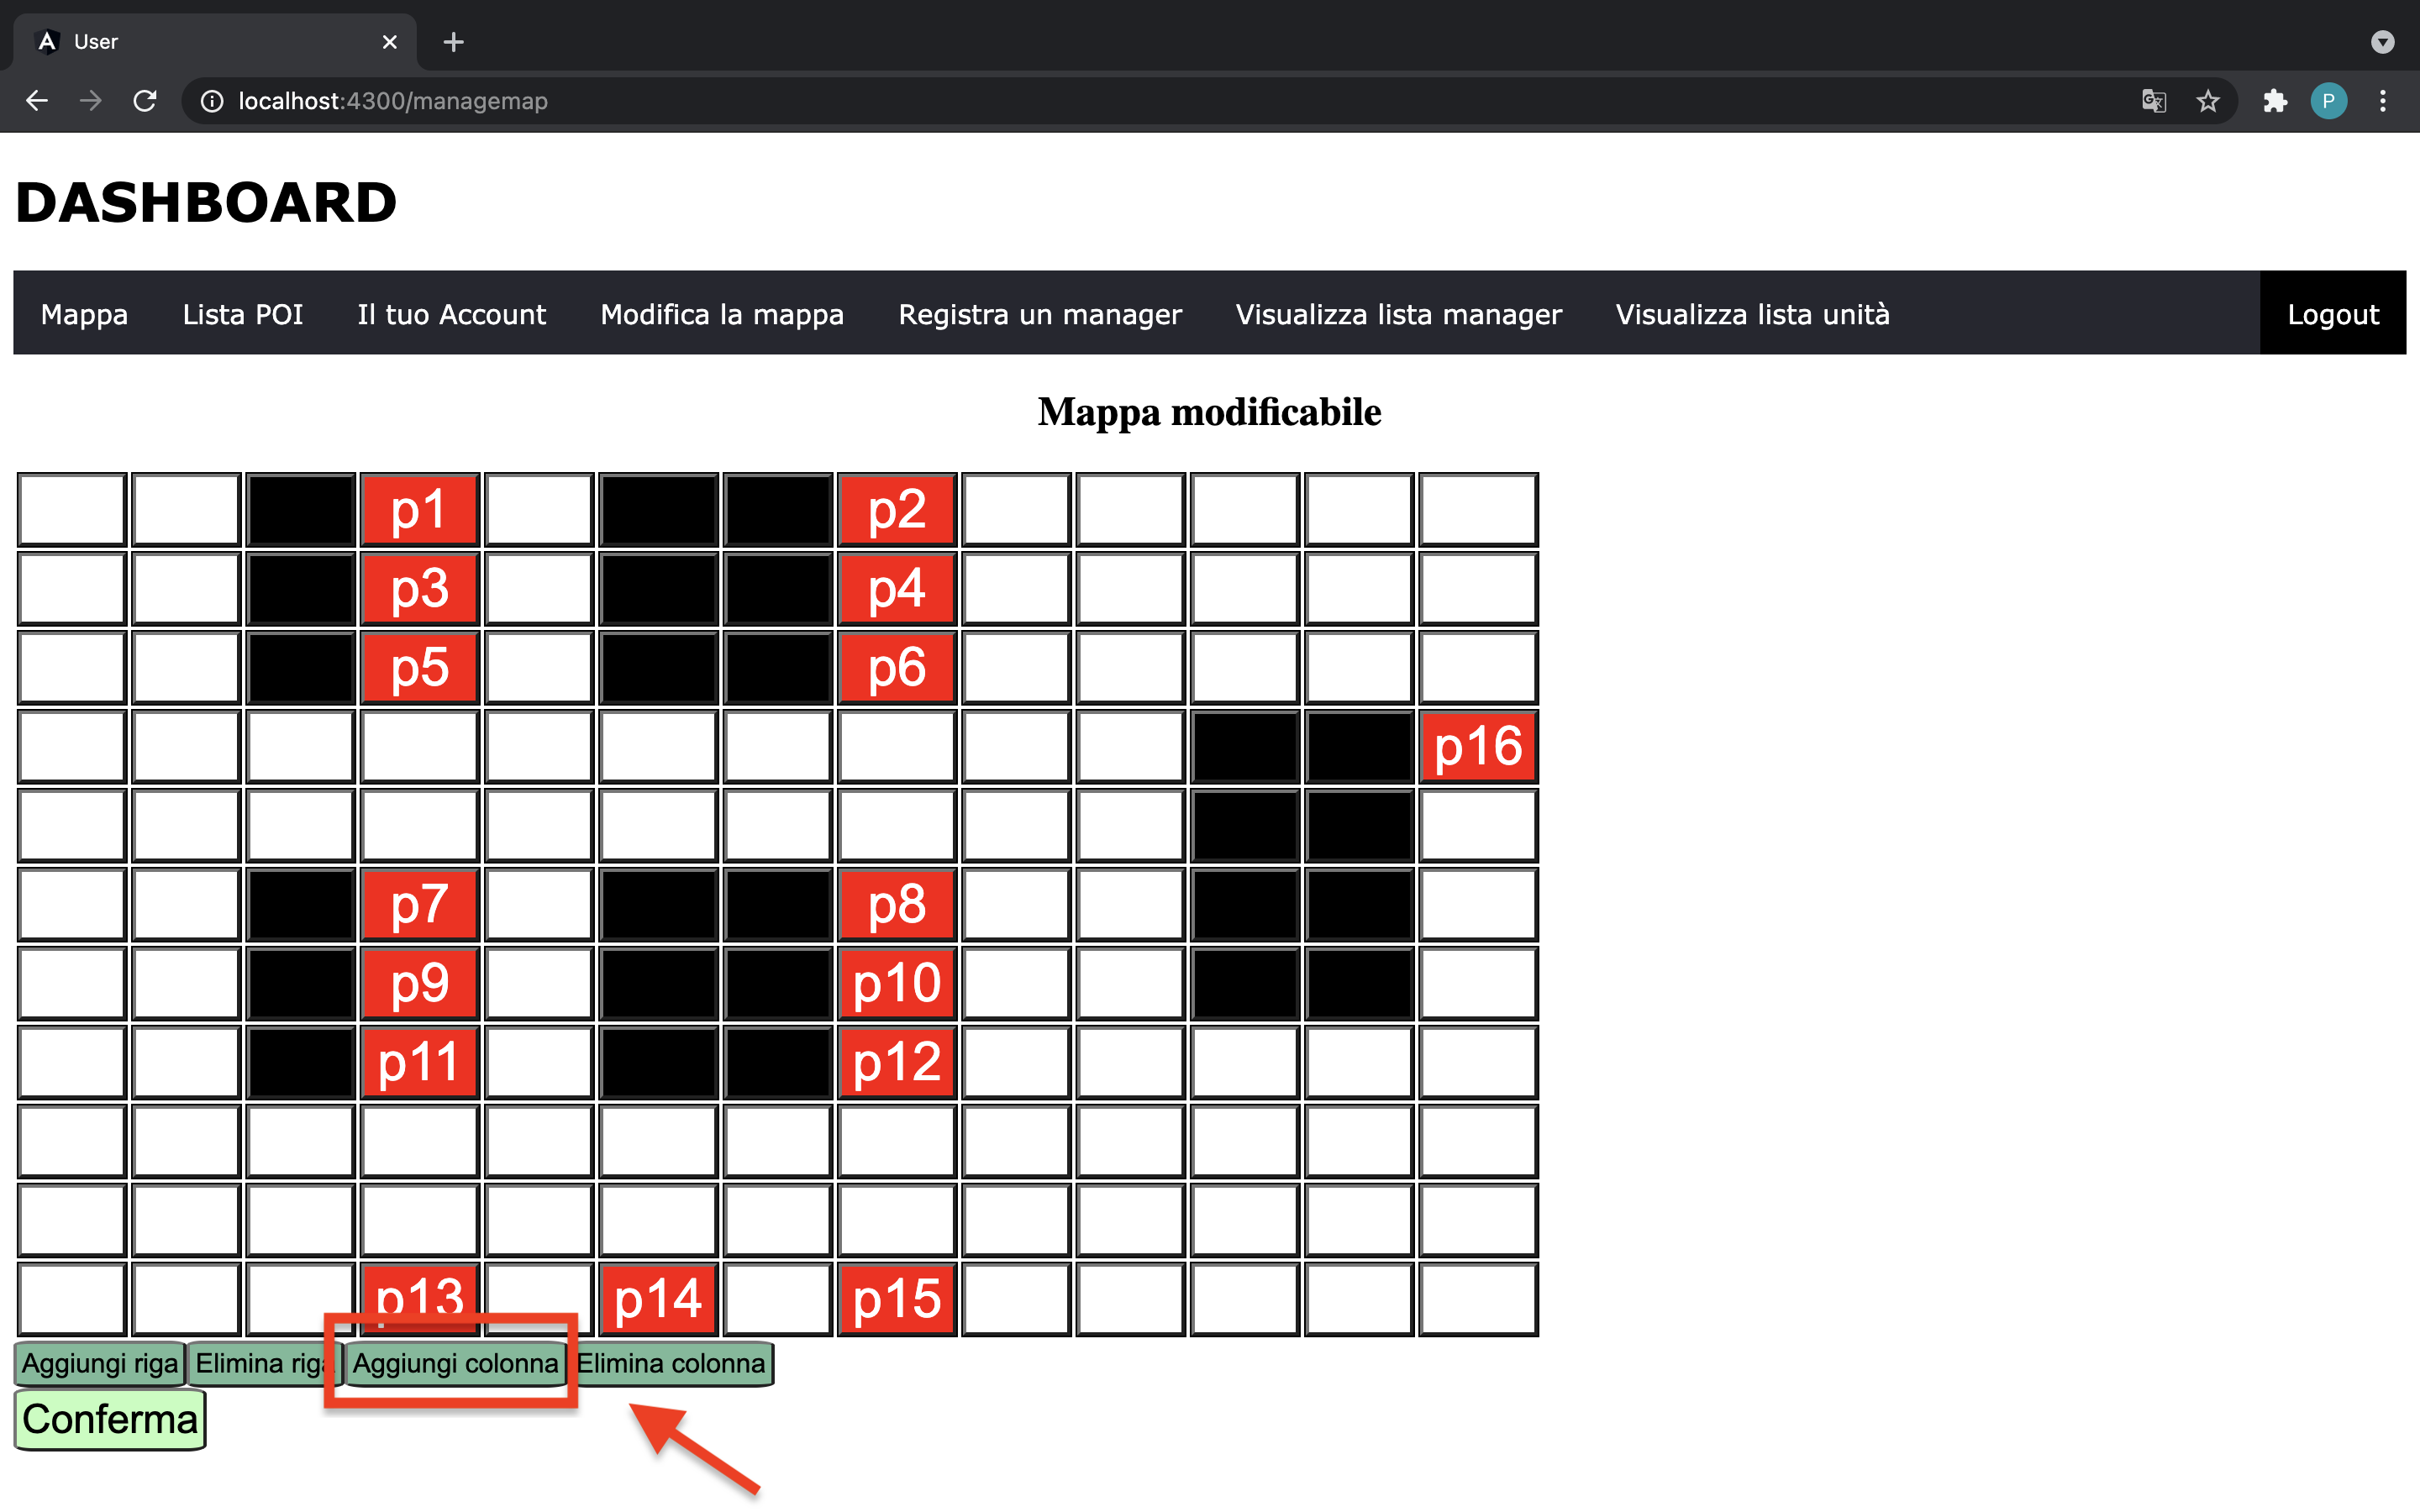
\includegraphics[scale=0.12]{res/images/modificamappa3.png}
                \caption{Istantanea dello schermo ampliamento mappa per colonna}
            \end{figure}
            \item eliminare una colonna: \\premere sul pulsante "Rimuovi colonna" per diminuire la planimetria di una colonna. Eliminare i POI presenti nell'ultima colonna prima di premere il pulsante altrimenti verrà visualizzato un errore e la cancellazione non verrà eseguita;
            \begin{figure}[H]
                \centering
                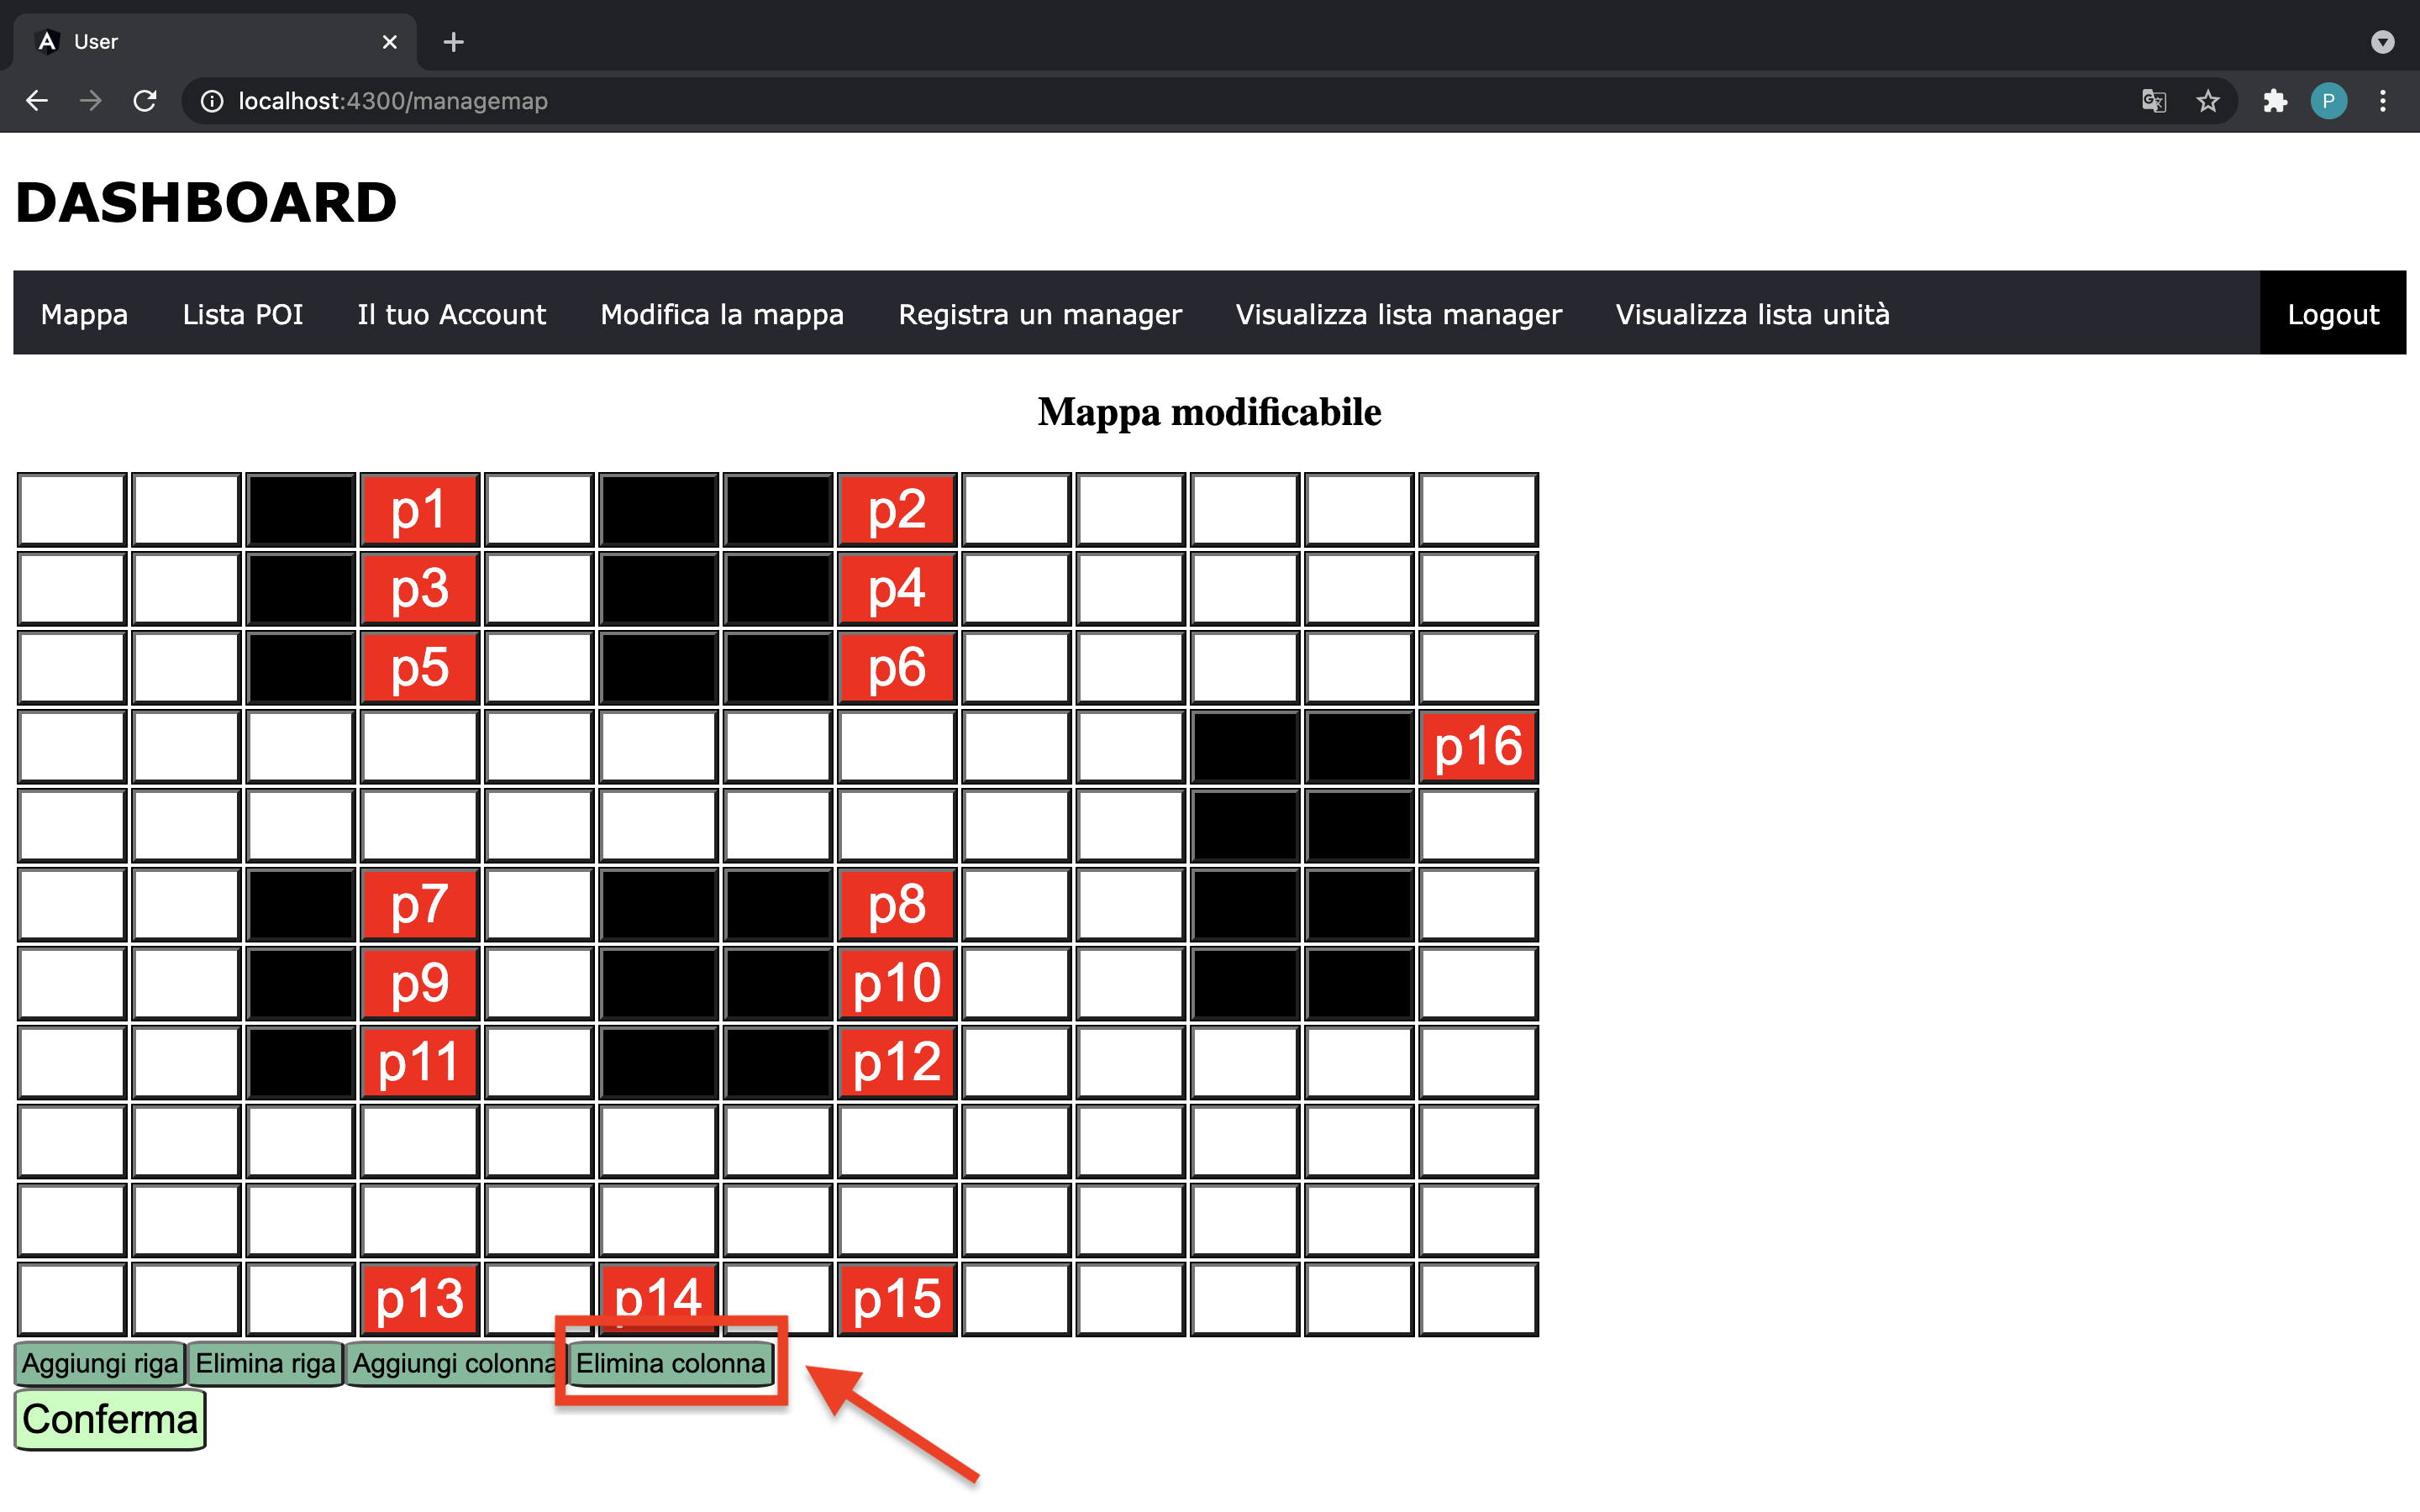
\includegraphics[scale=0.12]{res/images/modificamappa4.png}
                \caption{Istantanea dello schermo diminuzione mappa per colonna}
            \end{figure}
            \item cambiare il tipo di cella: \\premere sulla cella nella mappa che si intende modificare. Verrà allora visualizzata un'interfaccia con i colori possibili (bianco: zona transitabile, nero: zona non transitabile, frecce: sensi unici, rosso: POI di carico, marrone: POI di scarico, blu: POI di base). 
            \begin{figure}[H]
                \centering
                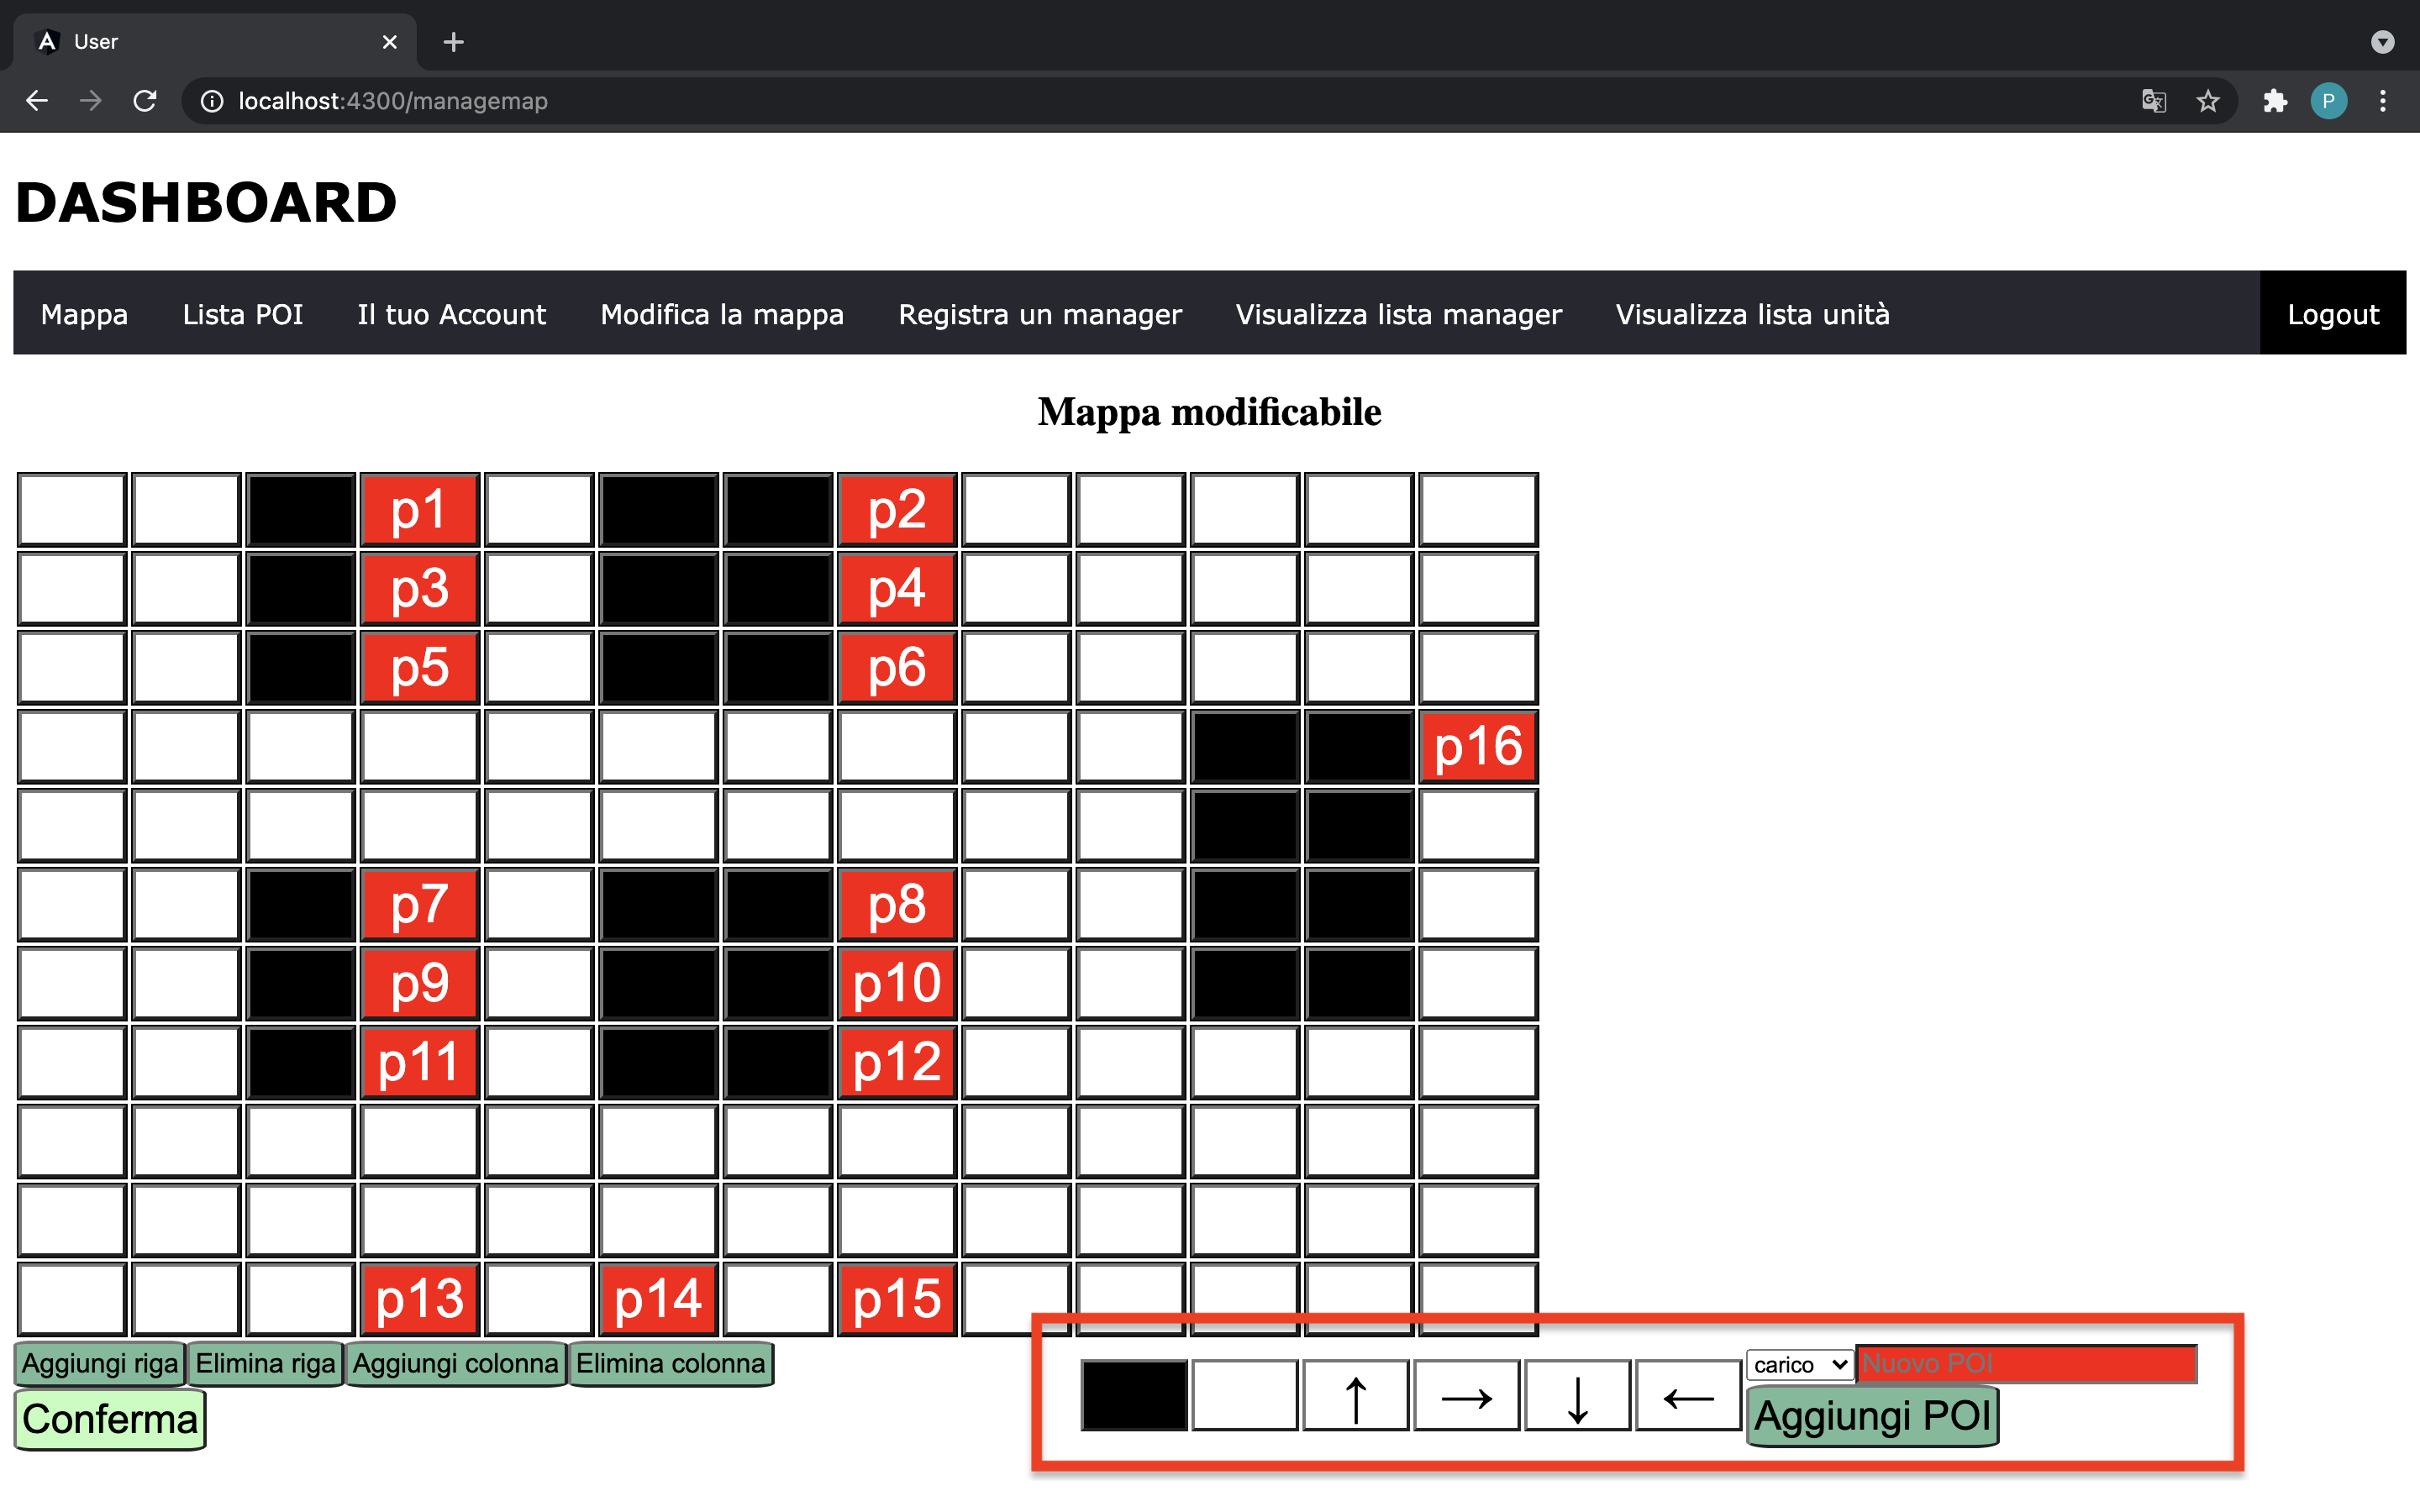
\includegraphics[scale=0.12]{res/images/modificamappa5.png}
                \caption{Istantanea dello schermo modifica tipo di cella}
            \end{figure}
            Nel caso di aggiunta POI è possibile scrivere il nome e scegliere il tipo tra carico, scarico e base. \\Una volta scelto premere sul tasto "Aggiungi POI".
            \begin{figure}[H]
                \centering
                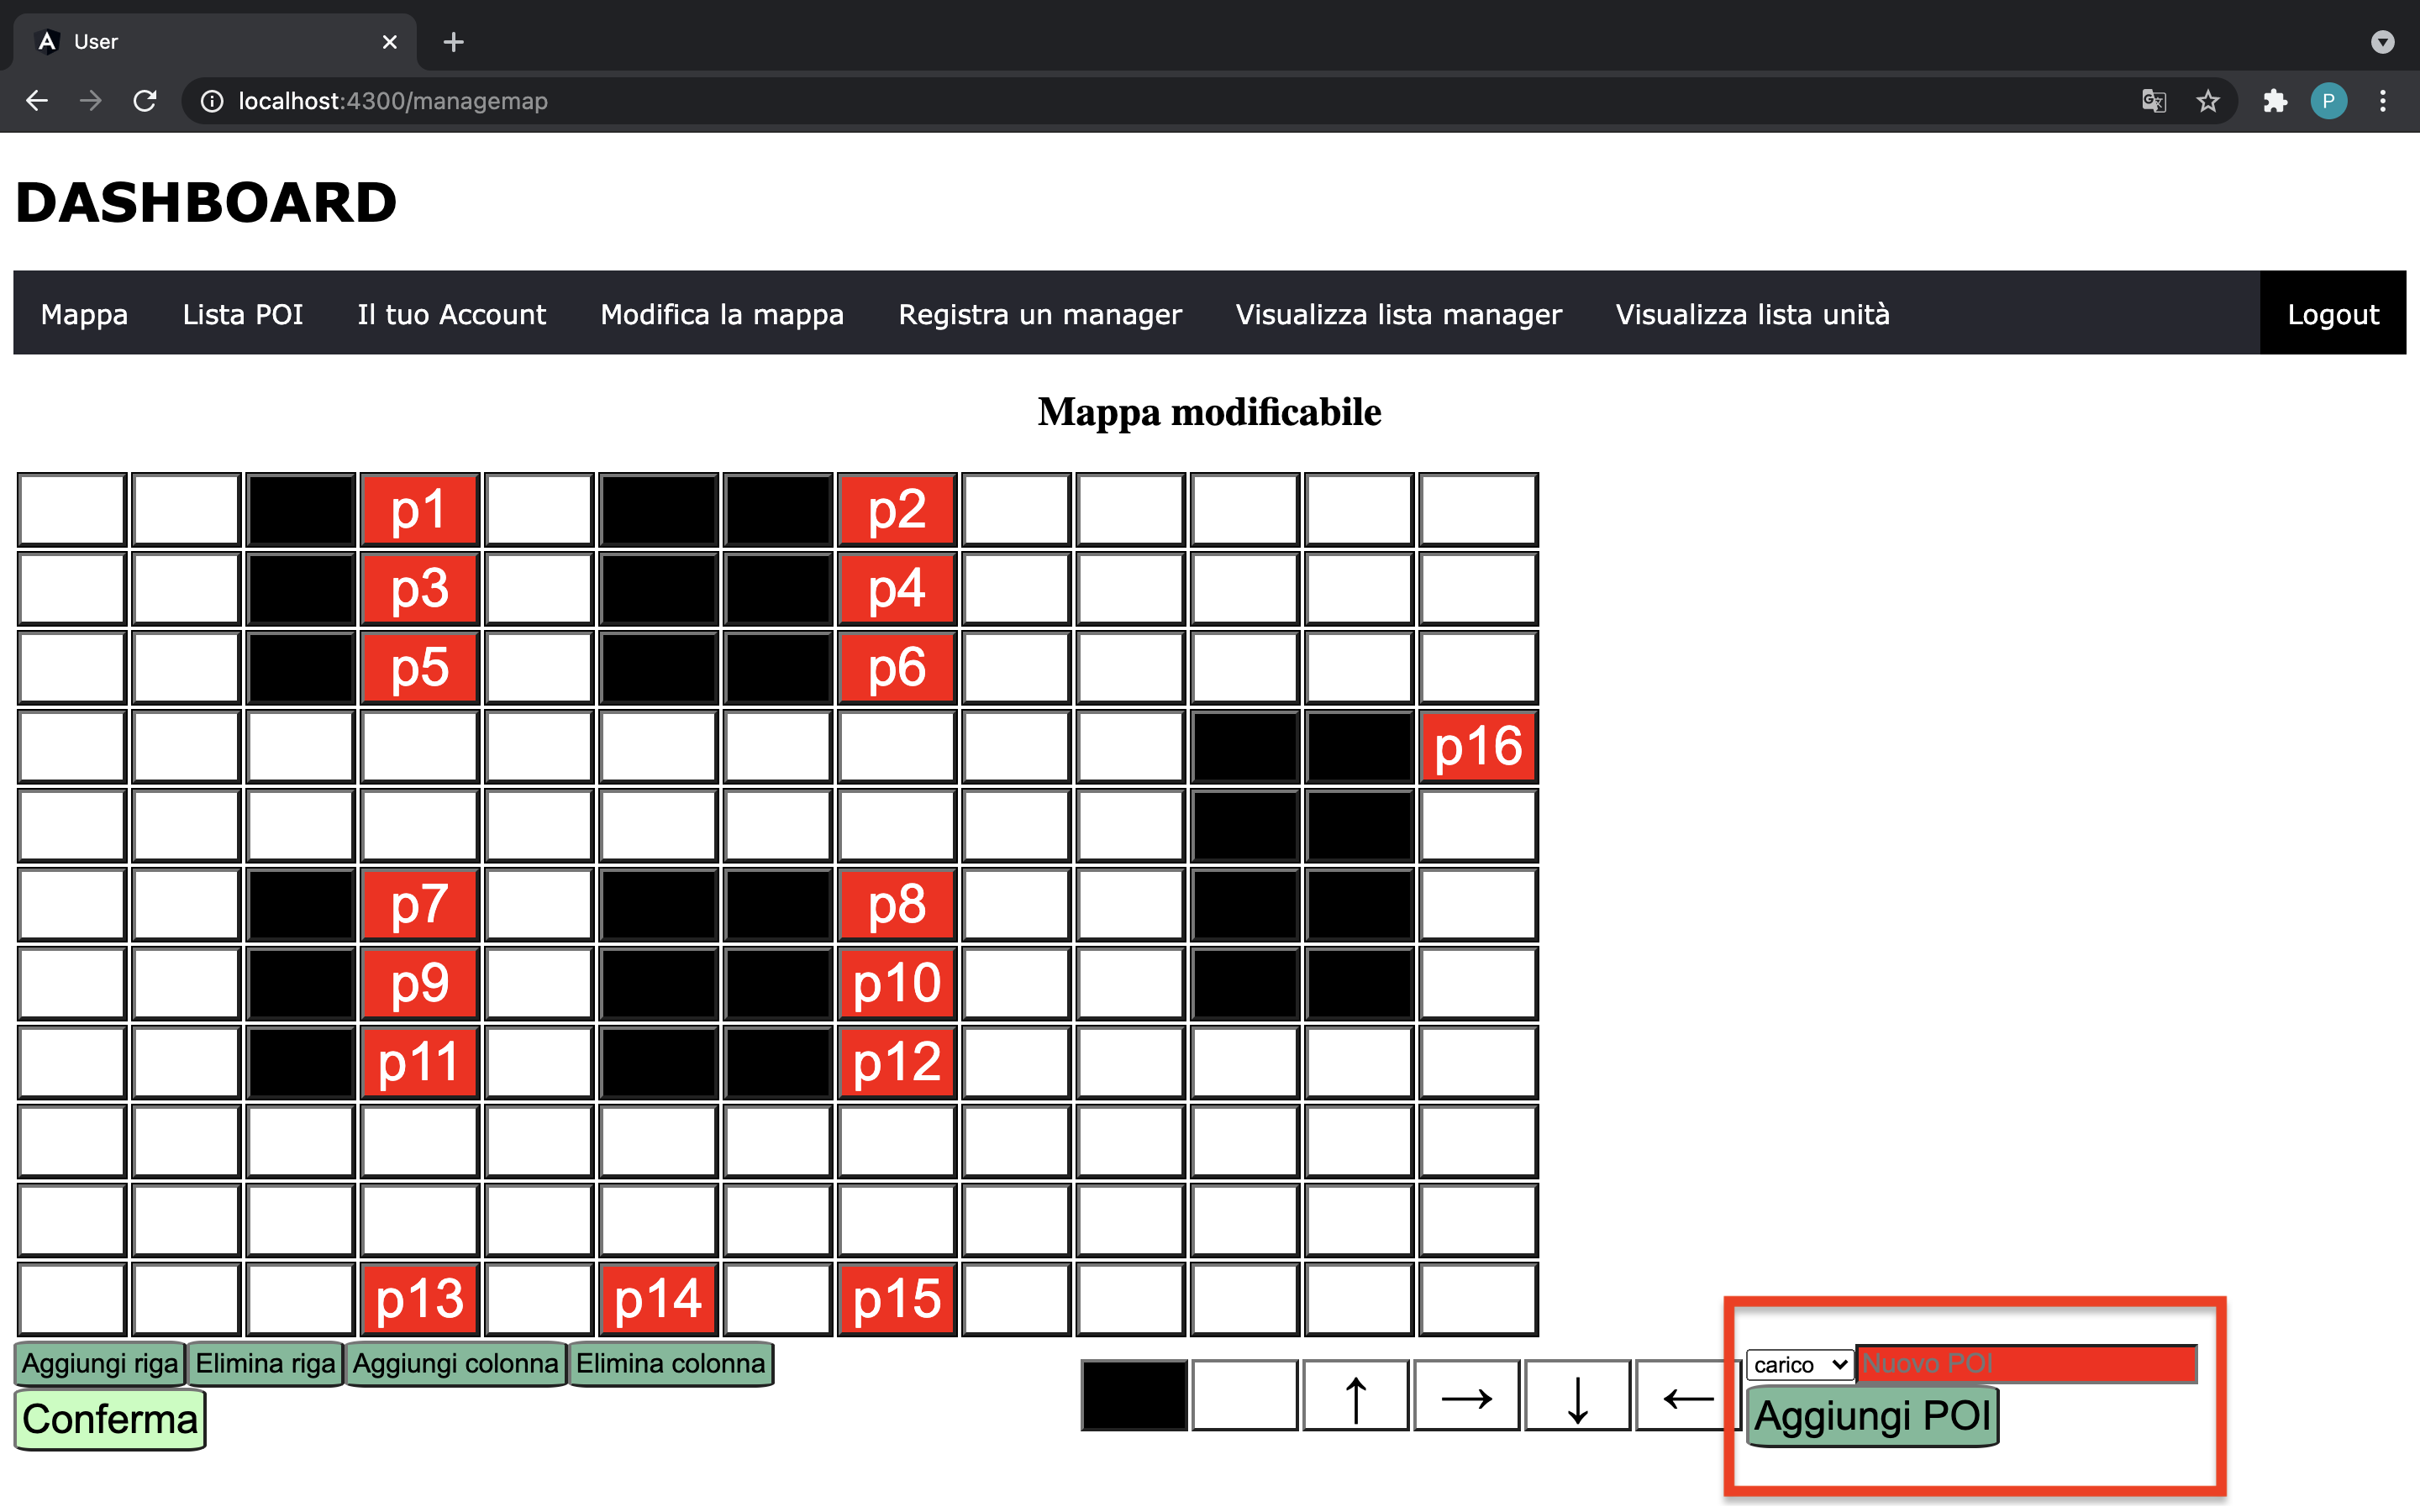
\includegraphics[scale=0.12]{res/images/modificamappa6.png}
                \caption{Istantanea dello schermo per aggiunta o modifica POI}
            \end{figure}
        \end{itemize}
        
    \item quando si è soddisfatti delle modifiche premere sul pulsante "Conferma".
    \begin{figure}[H]
        \centering
        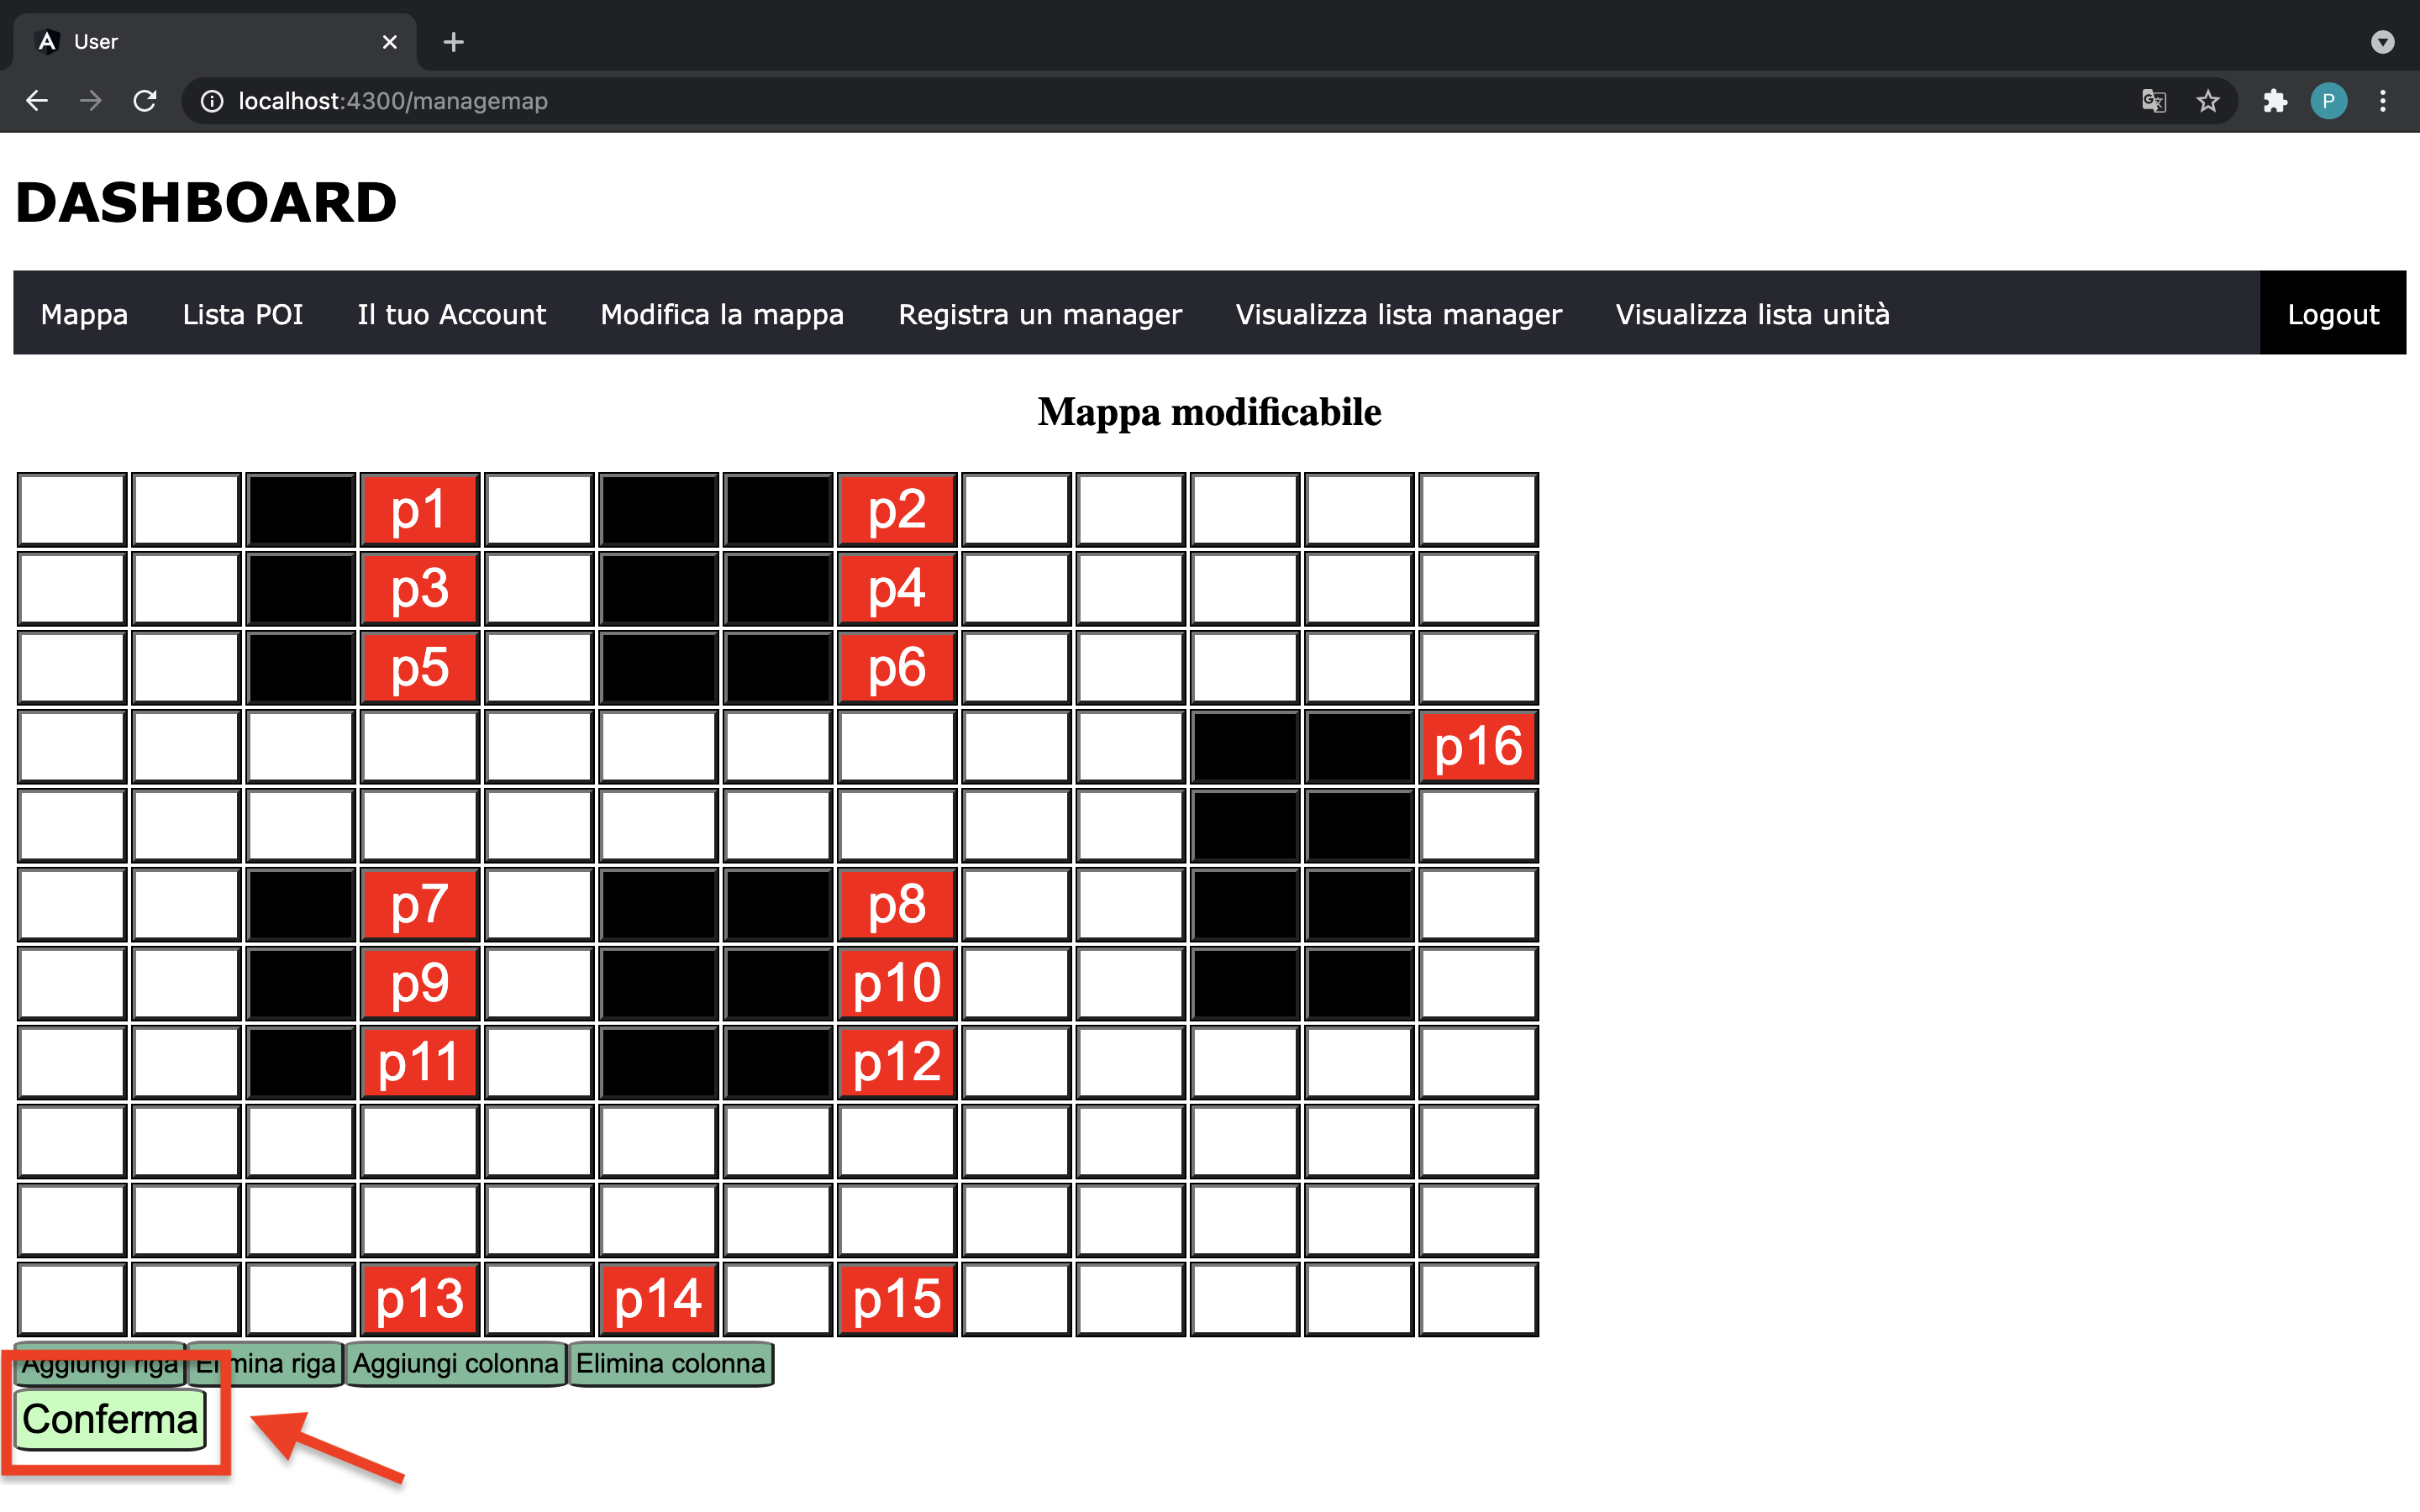
\includegraphics[scale=0.12]{res/images/modificamappa7.png}
        \caption{Istantanea dello schermo modifica mappa con conferma}
    \end{figure}
\end{itemize}



\subsection{Gestione unità}
\begin{itemize}
\item Dopo l'autenticazione, tramite il menù selezionare il pulsante "Visualizza lista unità"; 
\begin{figure}[H]
    \centering
    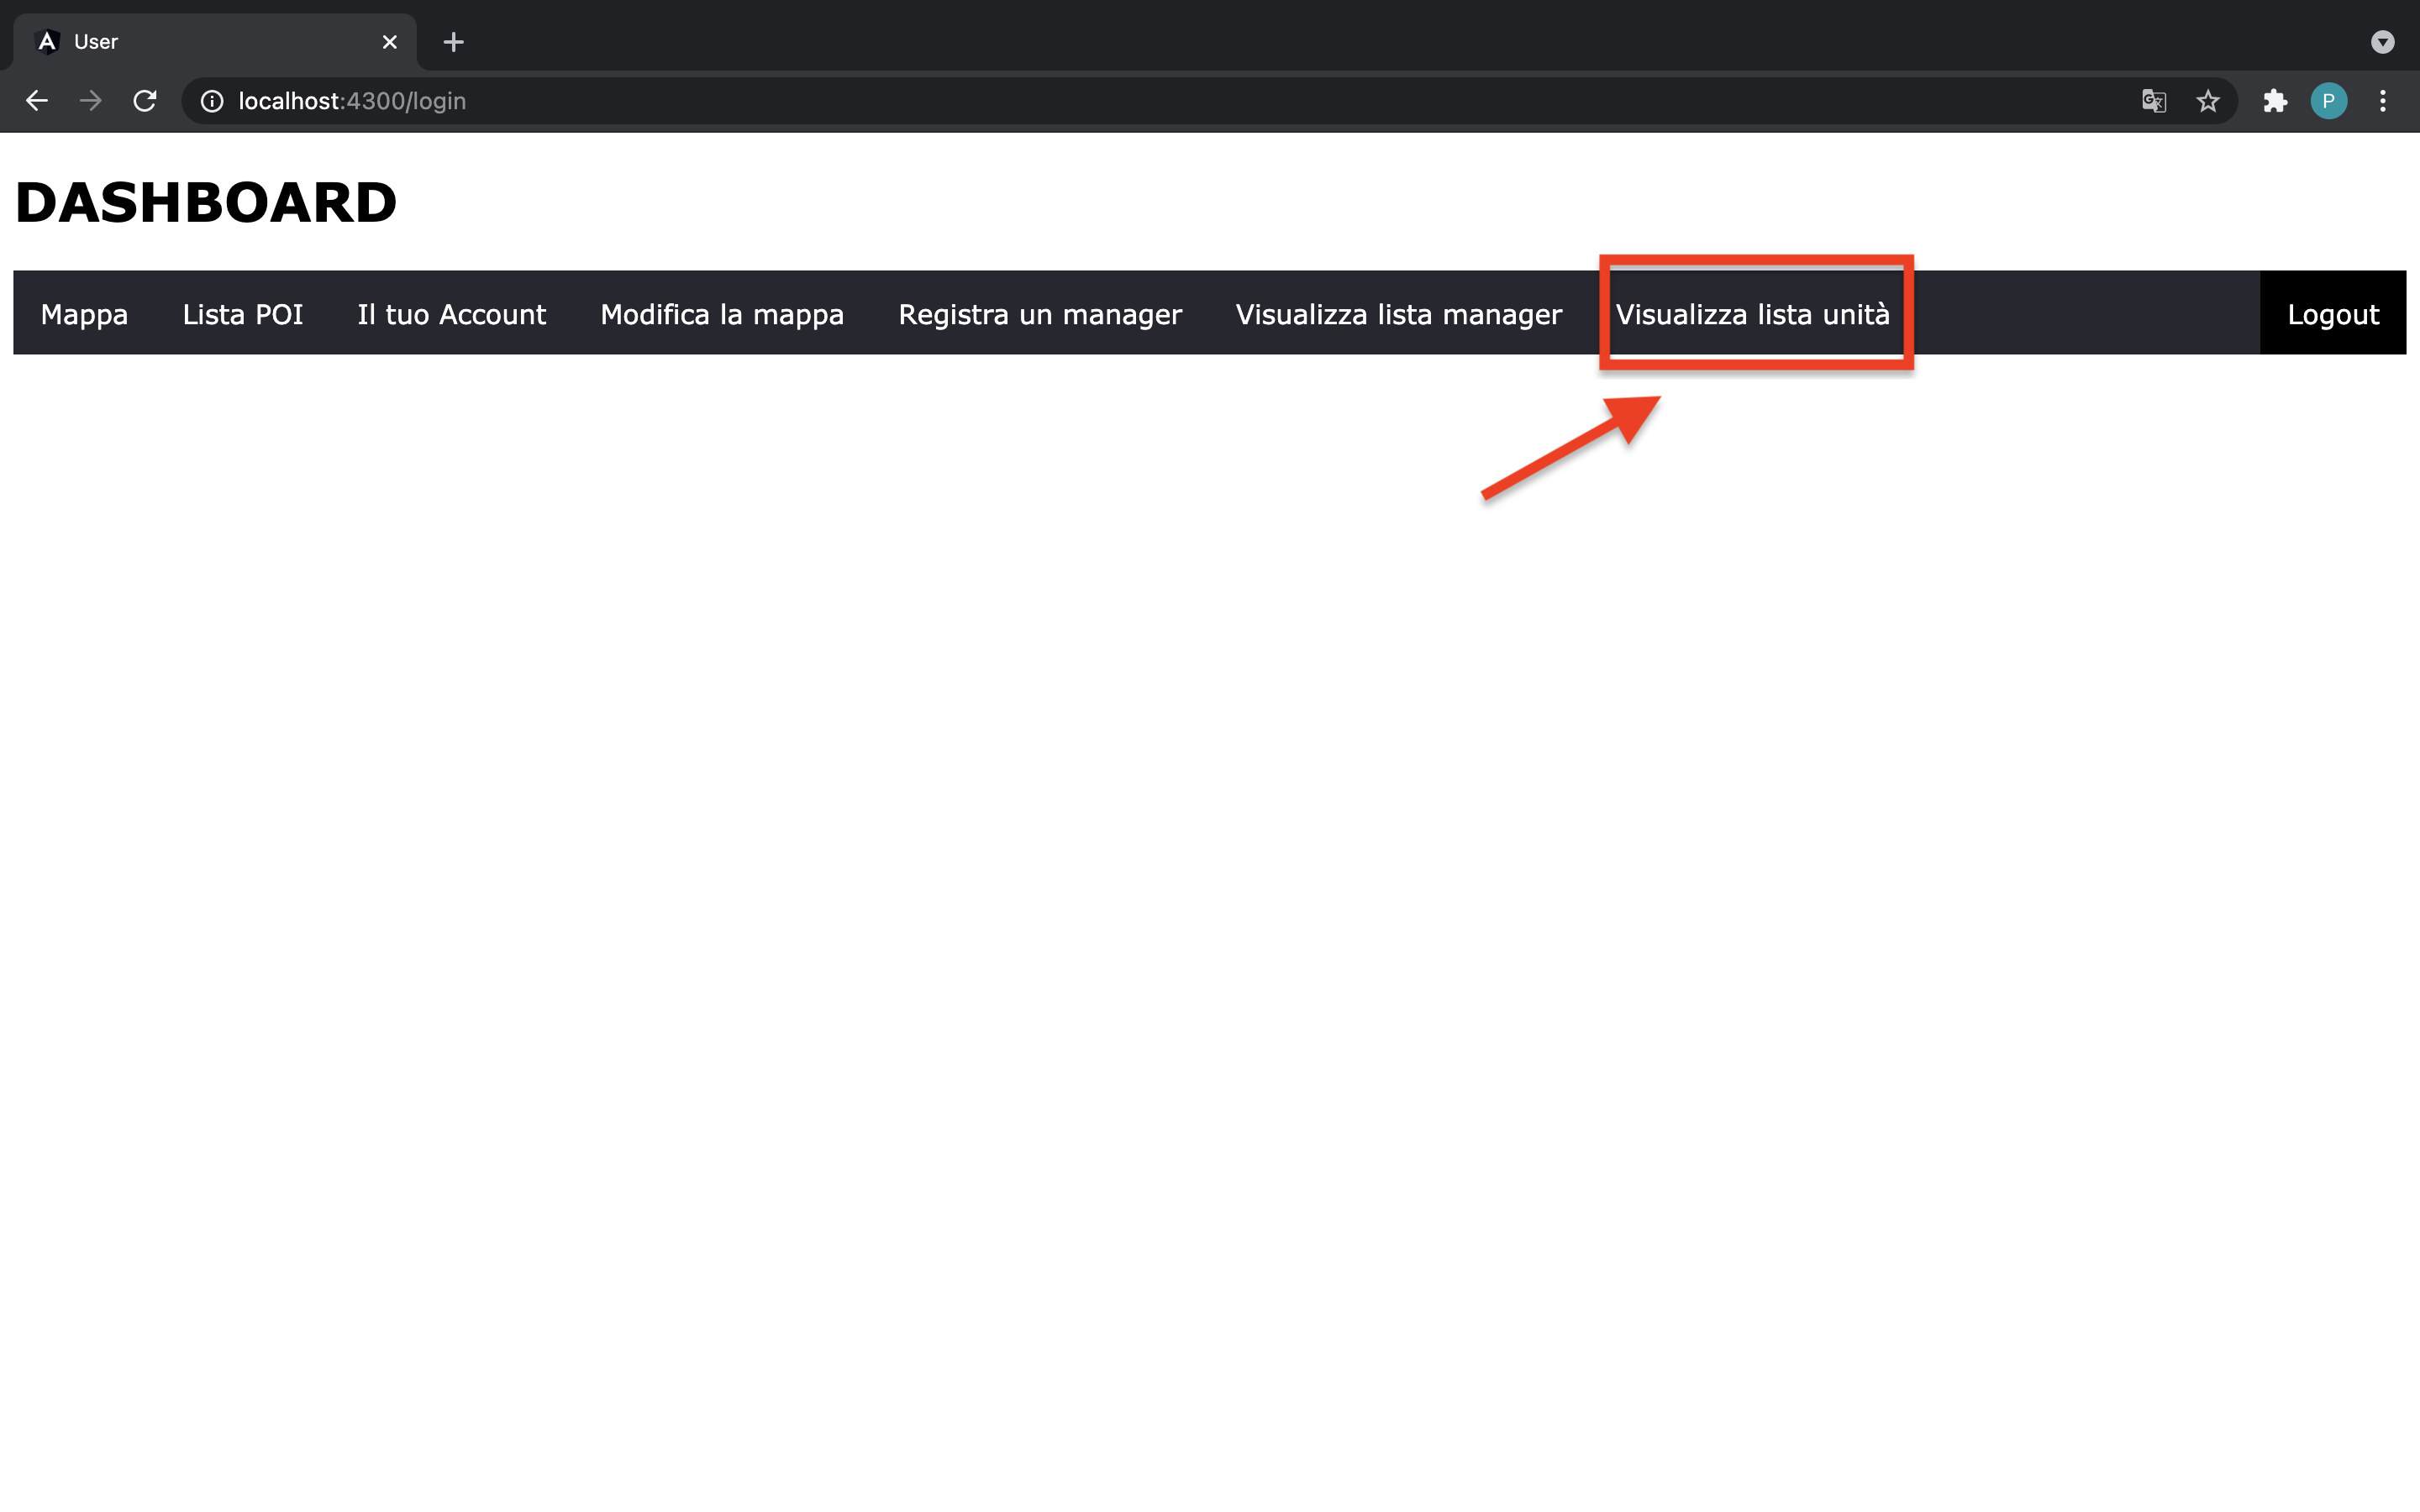
\includegraphics[scale=0.12]{res/images/dashboard7.png}
    \caption{Istantanea dello schermo lista unità}
\end{figure}
è possibile effettuare le seguenti operazioni:
    \item aggiungere una nuova unità: \\inserire il codice identificativo nel form e premere il pulsante "Registra";
    \begin{figure}[H]
        \centering
        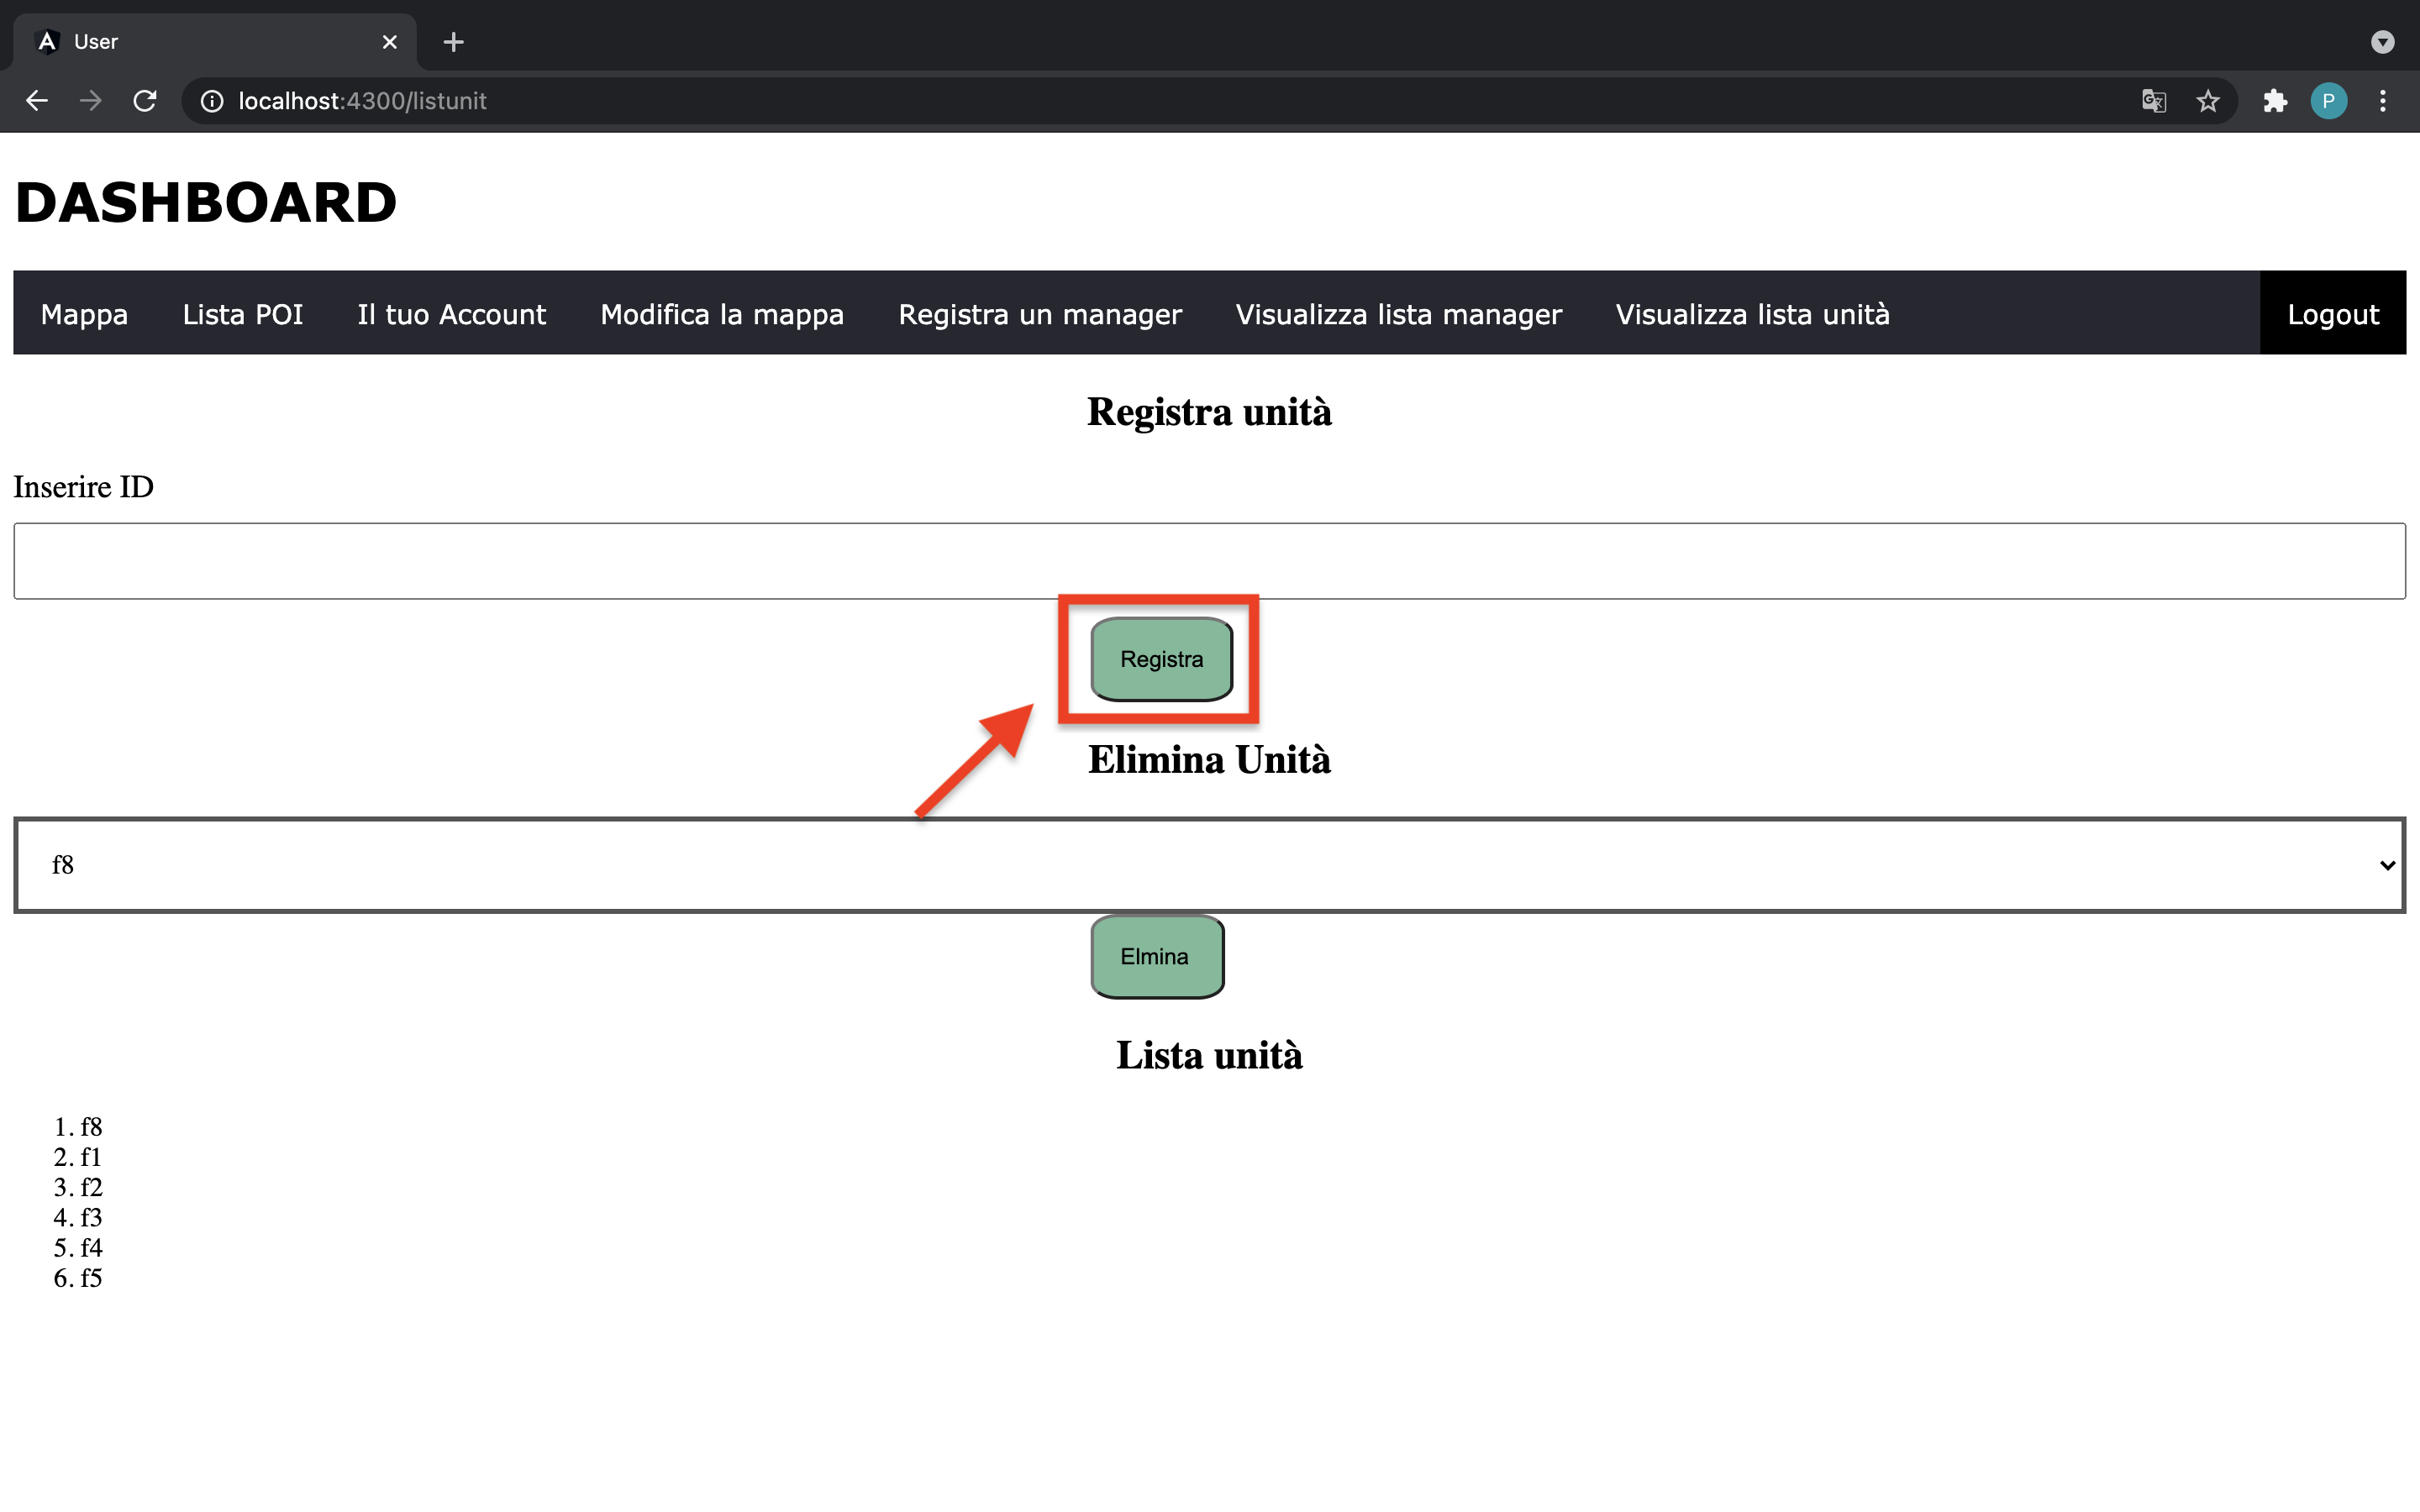
\includegraphics[scale=0.12]{res/images/nuovaunita.png}
        \caption{Istantanea dello schermo per l'aggiunta di una nuova unità}
    \end{figure}
    \item eliminare un'unità presente: 
    \begin{itemize}
        \item selezione dal menu a tendina l'id dell'unità che si intende eliminare;
        \item premere sul pulsante "Elimina" per confermare l'eliminazione.
    \end{itemize}
    \begin{figure}[H]
        \centering
        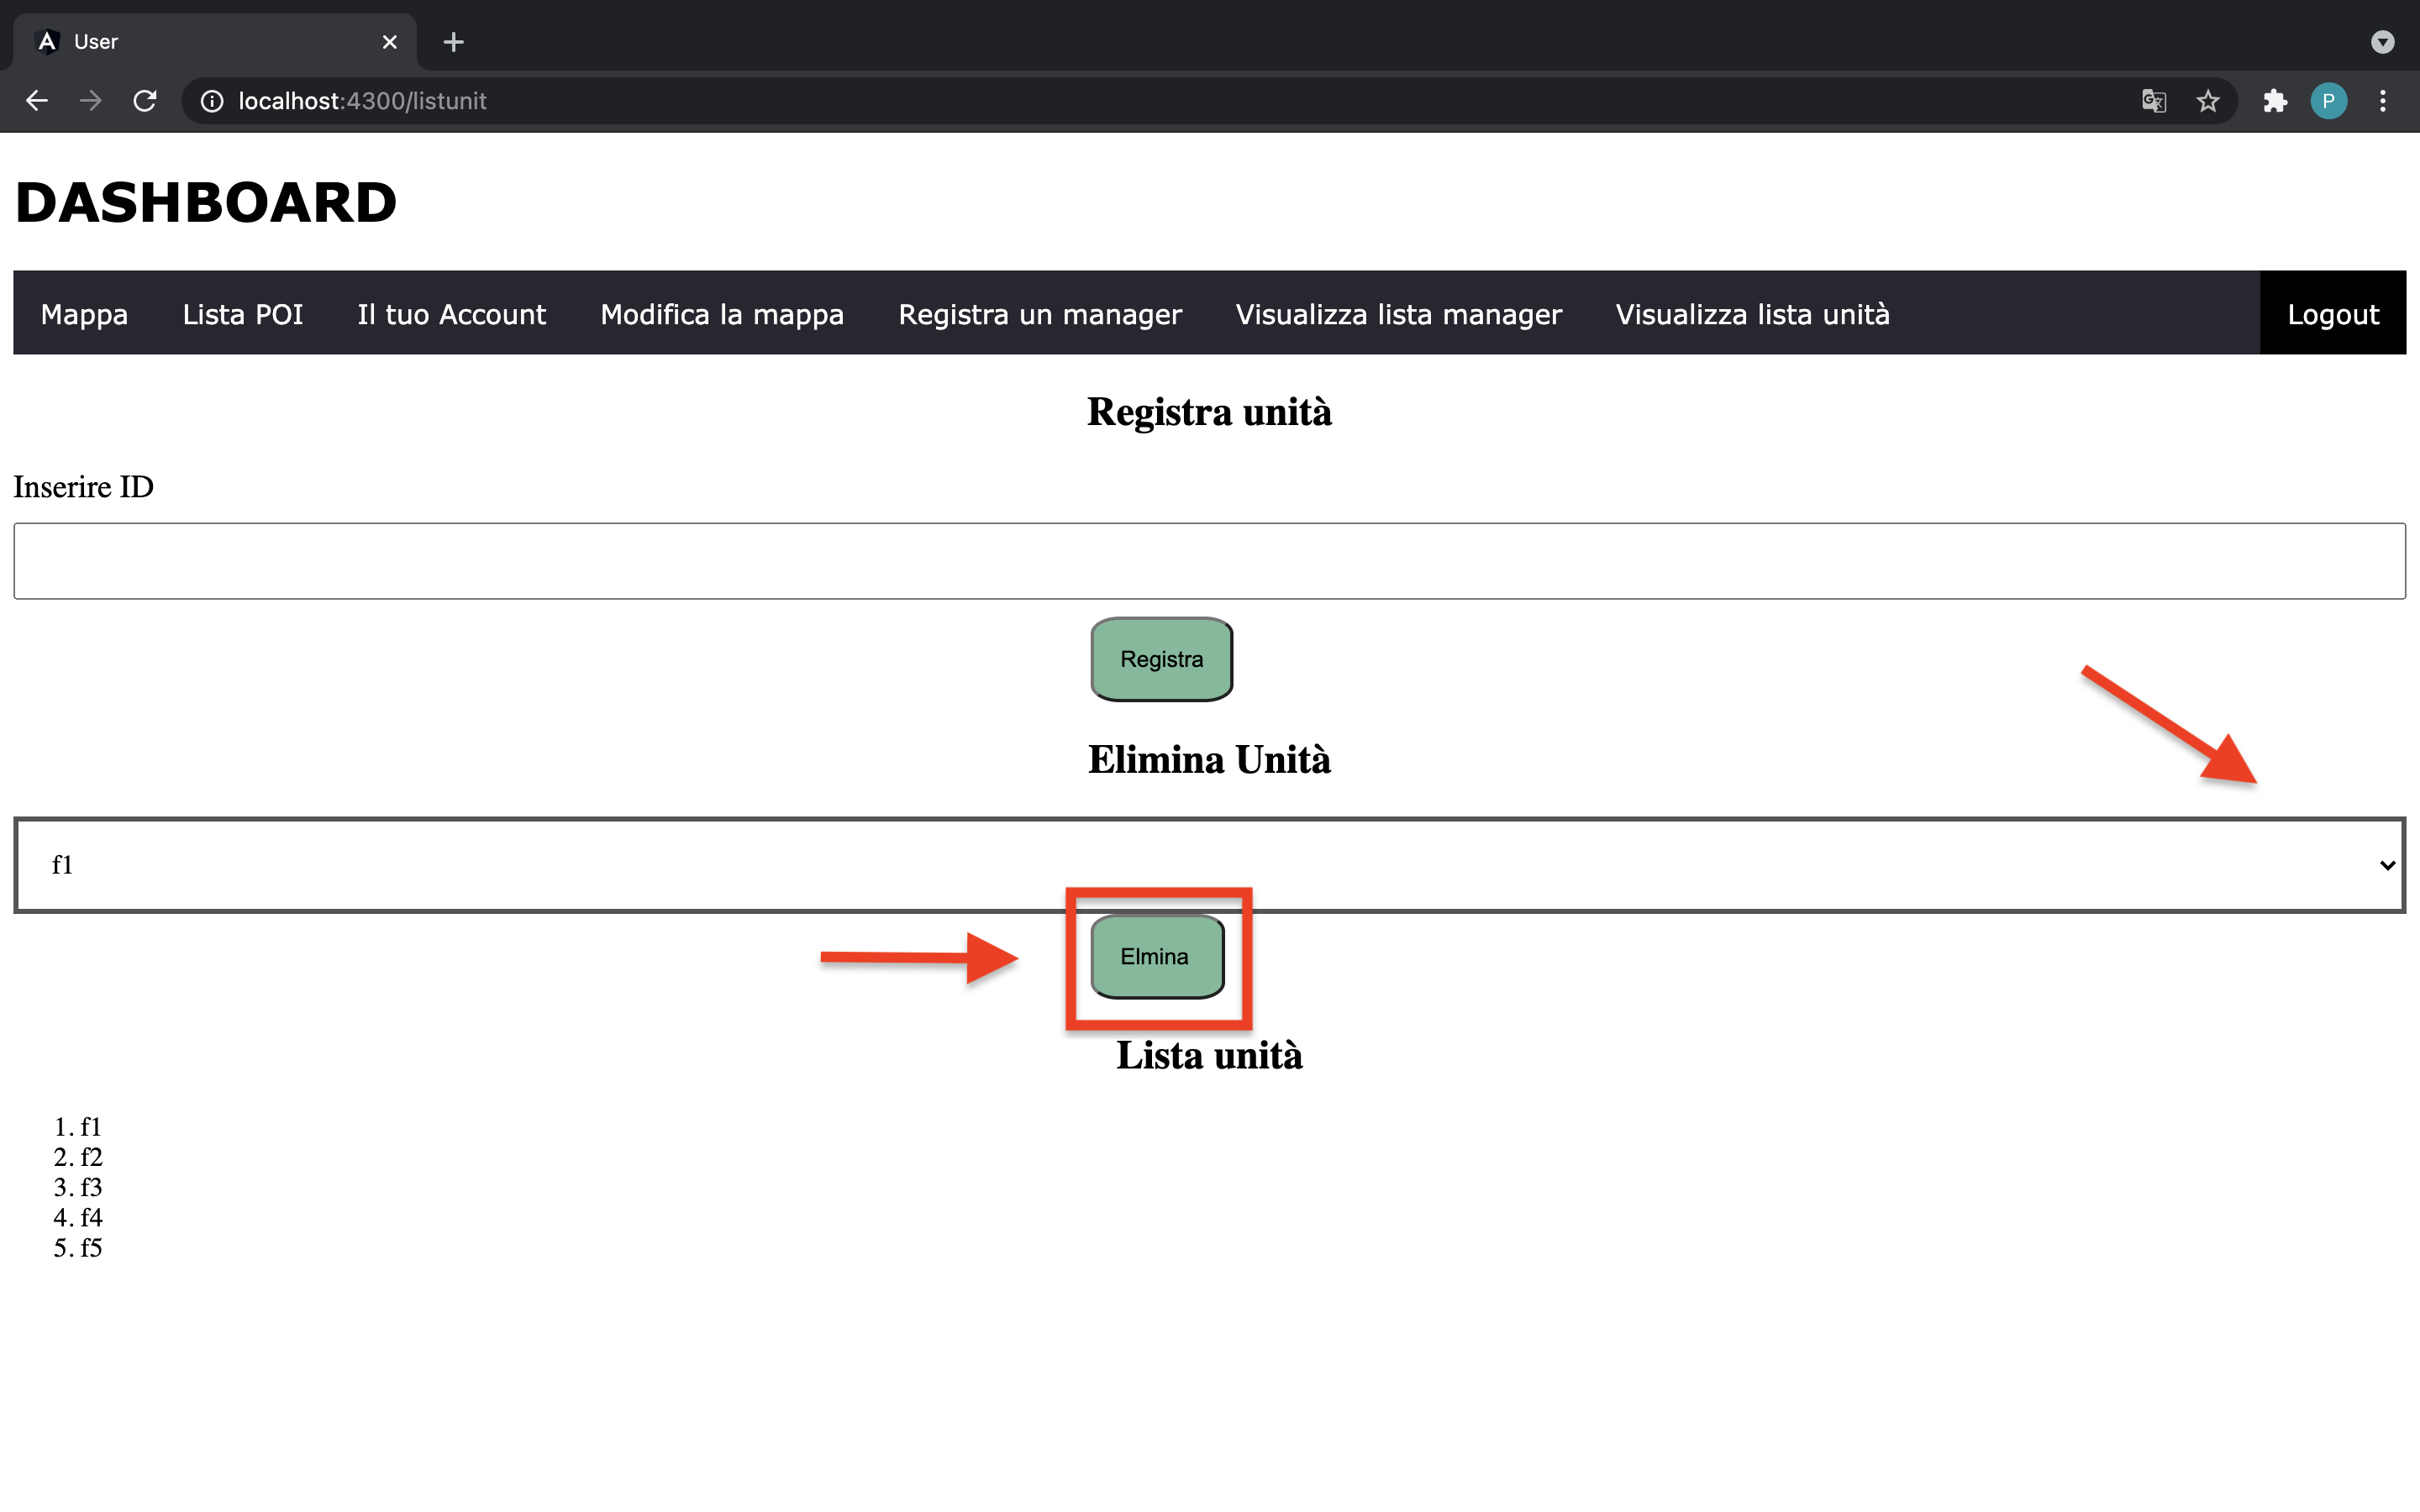
\includegraphics[scale=0.12]{res/images/eliminaunita.png}
        \caption{Istantanea dello schermo per l'eliminazione di un'unità}
    \end{figure}
\end{itemize}

\subsection{Logout}
\begin{itemize}
    \item Dopo l'autenticazione, tramite il menù selezionare il pulsante "Logout" per disconnettersi dall'applicativo e tornare alla pagina di login.
\end{itemize}
\begin{figure}[H]
    \centering
    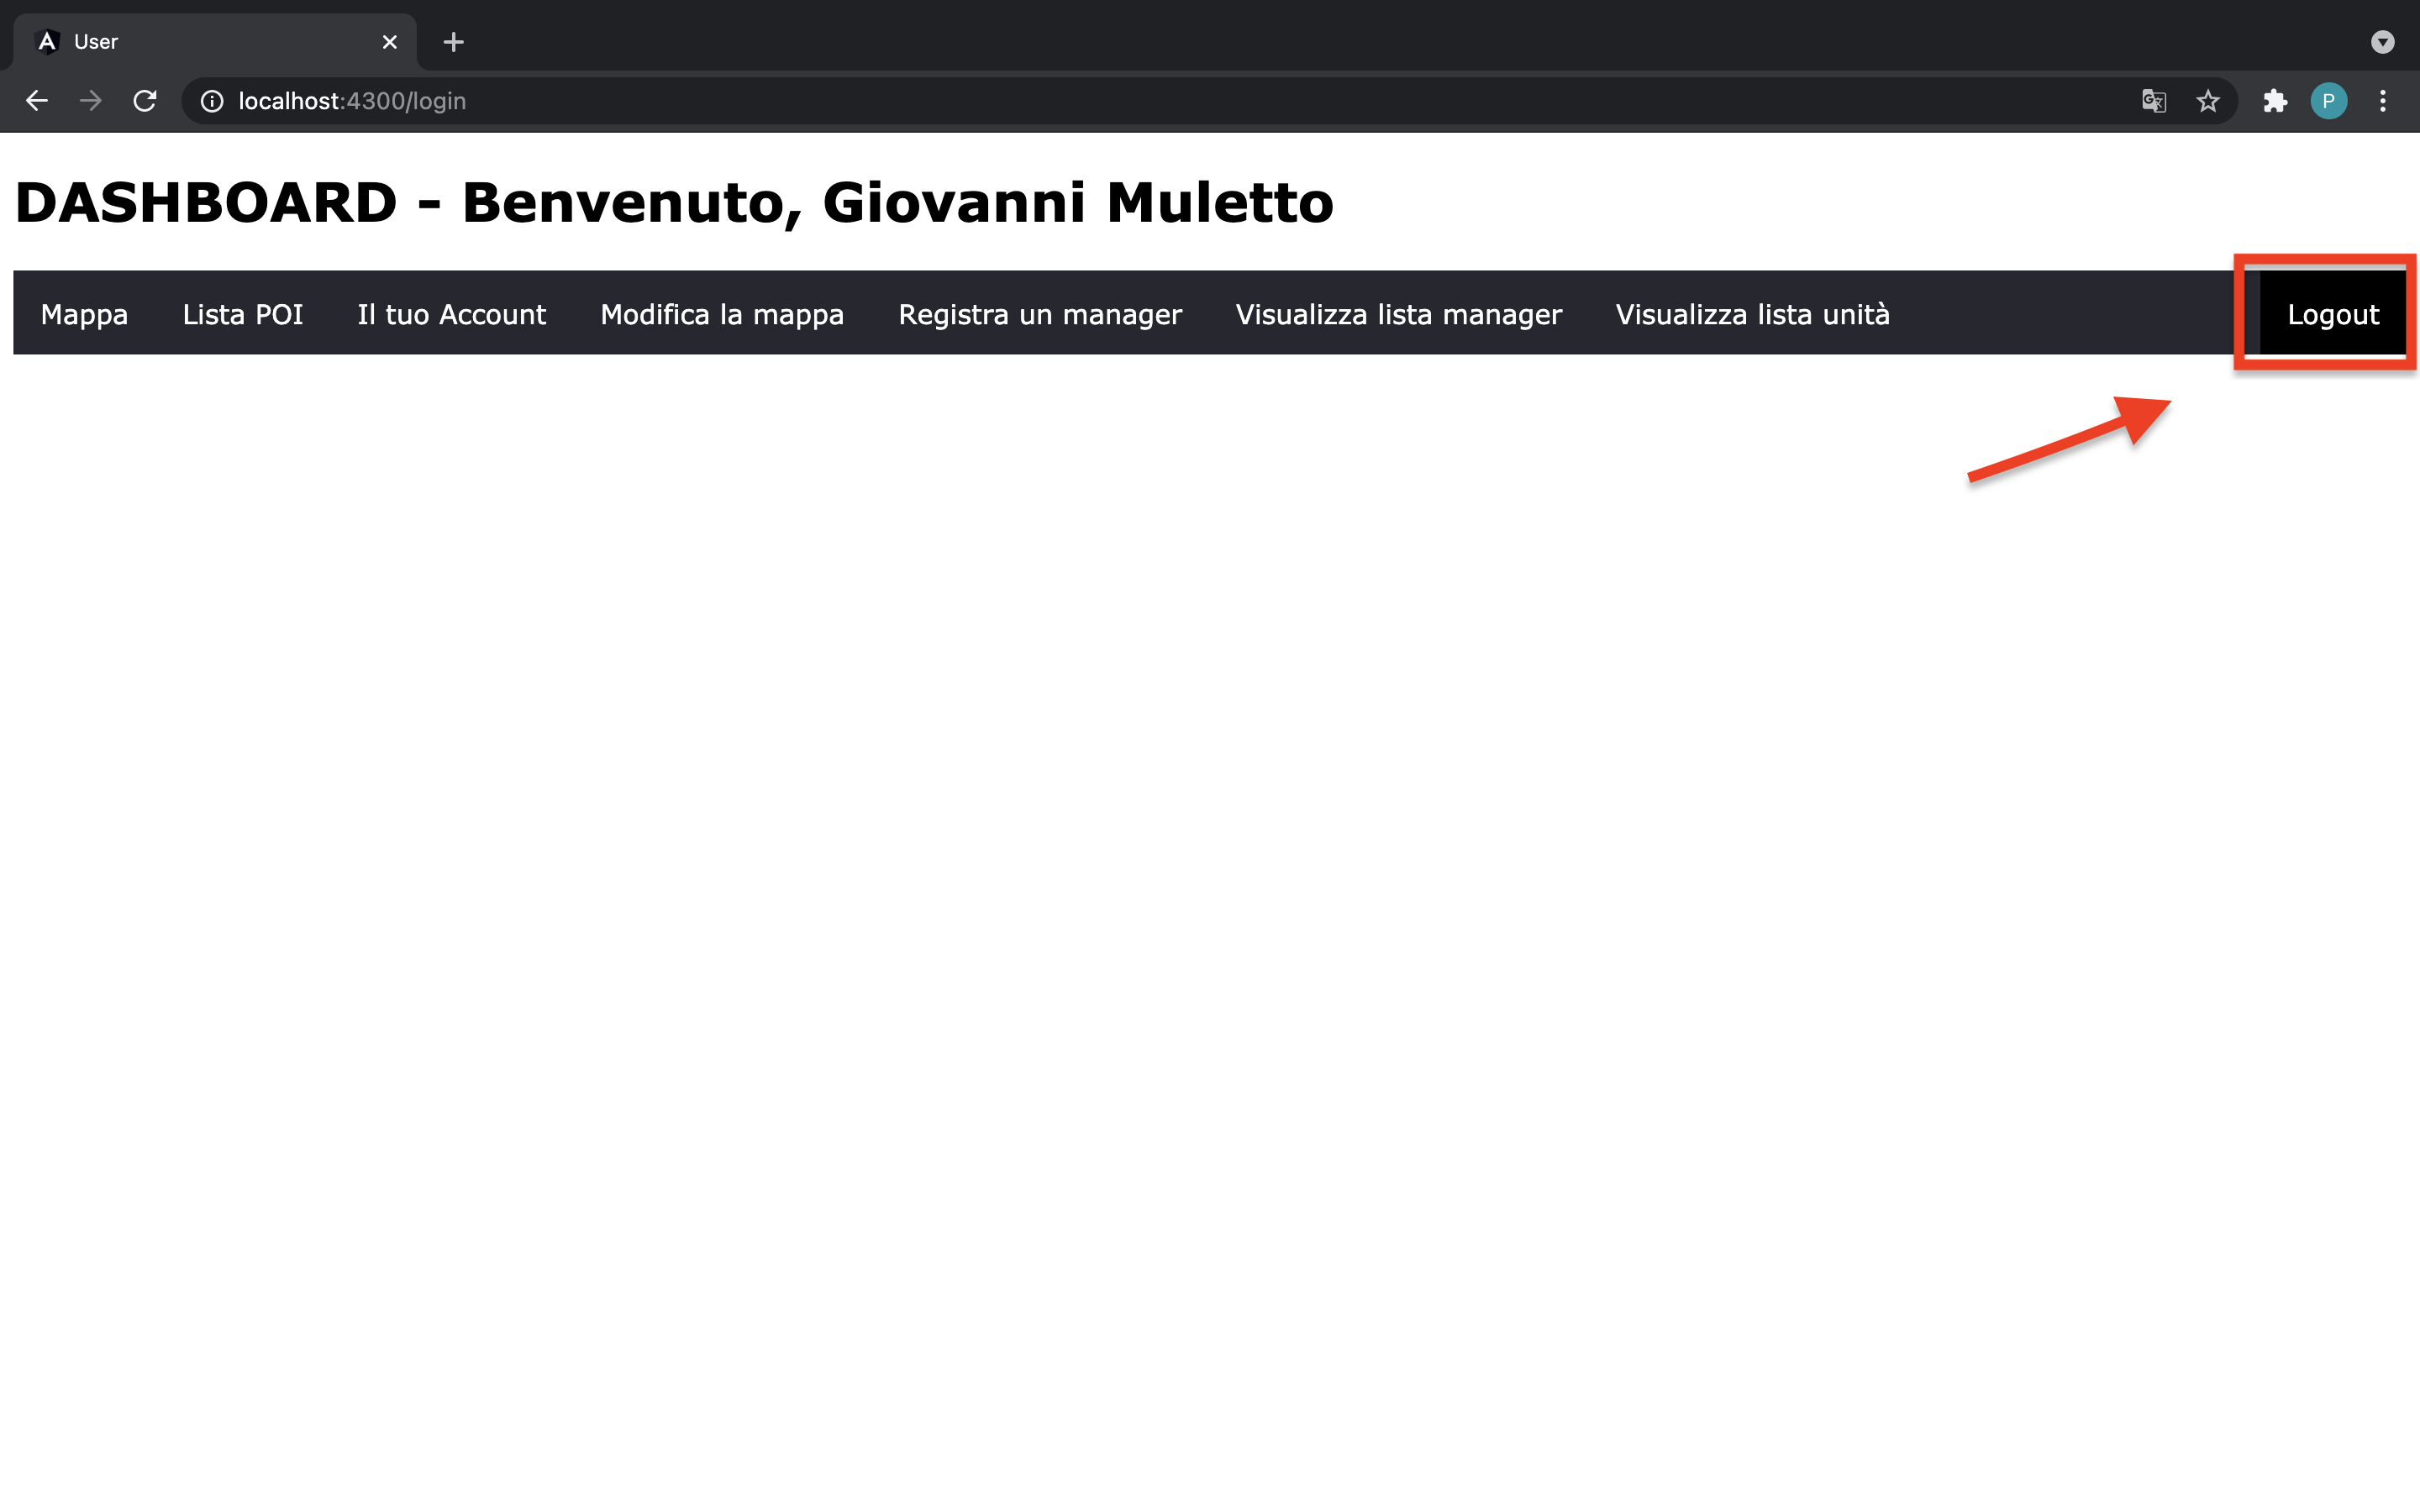
\includegraphics[scale=0.12]{res/images/logout.png}
    \caption{Istantanea dello schermo dashboard con indicazione per il logout}
\end{figure} 
